%
% Szablon do pracy inżynierskiej, zgodny z Załącznikiem nr 1 do Zarządzenia Rektora PG nr 17/2014 z 1 kwietnia 2014 r. 
% Wersja 1.11
% Autor: Mateusz Kraiński
% Kontakt w razie pytań: mt.krainski@gmail.com
% 
% Poza ustawieniem formatowania... wszystkiego, dodano metody ułatwiające właściwe formatowanie niektórych elementów kluczowych. Polecam zapoznać się z tym co jest dostępne.
% 
%
%
%
%
%
% Umieszczenie początku rozdziału, sekcji wraz z nazwiskiem autora w spisie treści.
% \namedchapter[imię i nazwisko autora fragmentu]{Tytuł fragmentu}
% \namedsection[imię i nazwisko autora fragmentu]{Tytuł fragmentu}
% \namedsubsection[imię i nazwisko autora fragmentu]{Tytuł fragmentu}
%
% Przykład:
% \namedchapter[Mateusz Kraiński]{Wstęp i cel pracy} %-> z nazwiskiem
% \namedchapter{Wstęp i cel pracy} %-> bez nazwiska
% 
%
%
%
%
%
% Dodanie wykazu najważniejszych oznaczeń i skrótów. Lista jest automatycznie sortowana osobno dla oznaczeń matematycznych i skrótów:
% \begin{sortedlist}
%  	 \mathitem[sort_as]{symbol}{opis}    %Dodanie elementu - symbolu matematycznego
%  	 \shortitem{Skrót}{wyjaśnienie} 	 %Dodanie elementu - skrótu
%\end{sortedlist}
%
% Parametr sort_as jest parametrem opcjonalnym. Podaje się tam jako co nasz symbol ma być sortowany. W przypadku pominięcia, do pola sort_as wstawiana jest wartość pola symbol. Przydatne w przypadku używania znaków specjalnych (np. \hat{}), które występują na początku nazwy zmiennej (algorytm wtedy sortowałby po znakach po kolei $, \, h, a, t ...). Podobnie w przypadku znaków Greckich (niestety nie wiem jak one powinny być sortowane - czy po literach słowa (np. delta), czy zgodnie z alfabetem greckim osobno).
%  
%Przykład:
%\begin{sortedlist}
%   \mathitem{$s$}{droga w ruchu prostoliniowym, jednostajnie przyspieszonym [m],}
% 	\mathitem{$v_0$}{prędkość początkowa [m/s],}
%   \mathitem{$t$}{czas poruszania się ciała [s],}
% 	\mathitem{$a$}{przyspieszenie [m/s$^2$ ].}
%	\mathitem[$delta$]{$\delta[n]$}{delta Kroneckera, impuls jednostkowy (sortowane jako słowo delta)}
%	\mathitem[$\delta$]{$\delta[n]$}{delta Kroneckera, impuls jednostkowy (sortowane osobno)}
%\end{sortedlist}
% 
%
%
%
%
%
% Dodanie obrazka w sposób łatwy (jest wpisana ścieżka obrazków jako rys/, czyli należy stworzyć folder 'rys' w folderze, w którym są pliki główne i tam umieszczać obrazki). Ewentualnie można wywołać \graphicspath{ {"ścieżka_dostępu_do_plików"/} } i zmienić ścieżkę dostępu. 
%Metoda może stwarzać problemy ze względu na sposób generacji labelów -> nie są one widoczne przez program, więc nie działa podpowiadanie. Są one tworzone przy kompilacji. Możemy się do nich odwołać przez \ref{fig:label_obrazka}
%
% \InsertImageSimple[rozmiar]{nazwa_pliku}{tytuł}{label_obrazka} -> wstawiany obrazek ma rozmiar 0.0-1.0 szerokości linii (parametr rozmiar w zakresie 0.0-1.0)
% 
% \InsertImageSimple{nazwa_pliku}{tytuł}{label_obrazka} -> wstawiany obrazek ma rozmiar oryginalny
%
% Wstawianie obrazka "the hard way":
%
%\begin{figure}[h!tb]
%	 \centering
%	 \includegraphics[width = 1.0\linewidth]{logoPG}
%	 \caption{logo PG}
%	 \label{fig:labPG}
%\end{figure}
% 
%
%
%
%
%
% Dodanie dwóch obrazków obok siebie, zasady podobne jak wyżej.
% \InsertSubImagesSimple
%	{nazwa_pliku_obrazek1}
%	{tytuł_obrazek1}
%	{label_obrazek1}
%	{nazwa_pliku_obrazek2}
%	{tytuł_obrazek2}
%	{label_obrazek2}
%	{tytuł_całość}
%	{label_całość}
%
% Przykład z wykorzystaniem obrazków logoETI i logoPG tworzy etykiety fig:ETI, fig:PG i fig:logos:
% \InsertSubImagesSimple
%	{logoETI}		%nazwa_pliku_obrazek1
%	{ETI}			%tytuł_obrazek1
%	{ETI}			%label_obrazek1
%	{logoPG}		%nazwa_pliku_obrazek2
%	{PG}			%tytuł_obrazek2
%	{PG}			%label_obrazek2
%	{Loga}			%tytuł_całość
%	{logos}			%label_całość
%
% Dodanie obrazków obok siebie "the hard way". Proszę korzystać z realCaptionx i tam wpisywać tytuły obrazków ze względu na wymagane formatowanie. Można powiedzieć, że to wersja beta - nie było za bardzo testowane, ale działało:
% 
% \begin{figure}[h!tb] 
%	\centering
%   \def\realCaptionA{tytuł_obrazek1}
%	\def\realCaptionB{tytuł_obrazek2}
%	\def\realCaptionAll{tytuł_całości}
%	\begin{subfigure}[t]{0.4\linewidth}
%		\caption{)}
%		\centering
%		\includegraphics[width = 1.0\linewidth]{plik_obrazek1}
%		\label{fig:lab1}		
%	\end{subfigure}
%	\quad
%	\begin{subfigure}[t]{0.4\textwidth}
%		\caption{)}
%		\centering
%		\includegraphics[width = 1.0\linewidth]{plik_obrazek2}
%		\label{fig:lab2}
%	\end{subfigure}
%	\def\showncap {\realCaptionAll\\ a) \realCaptionA, b) \realCaptionB}
%	\caption[\realCaptionAll]{\showncap}
%	\label{fig:labc}
% \end{figure}
% 
%
%
%
%
%
% Dodanie opisu zmiennych do równania \equationDescriptor i \equationDescriptorS. Druga funkcja dodatkowo sortuje alfabetycznie podane symbole (może to być przydatne przy skomplikowanych wzorach, ale nie przydatne przy prostych, gdzie zmienne podajemy w porządku pojawiania się). Składania podobna jak w sortedList, ale jest trochę inne formatowanie wynikowe.
%
% \begin{equationDescriptor}
% 	\EQDitem{symbol}{opis} -> EQation Descriptor item
% 	\EQDitem{symbol}{opis} 
% \end{equationDescriptor}
%
% Przykład:
% \begin{equation}
% 	s = v_0 \cdot t + \frac{a\cdot t^2}{2}
%   \label{eq:my_eq}
% \end{equation}
% gdzie:   				% nie należy zostawiać linii wolnej przed "gdzie:", gdyż spowoduje to rozpoczęcie tej linii od akapitu
% \begin{equationDescriptor}
%   \EQDitem{$s$}{droga w ruchu prostoliniowym, jednostajnie przyspieszonym [m],}
% 	\EQDitem{$v_0$}{prędkość początkowa [m/s],}
%   \EQDitem{$t$}{czas poruszania się ciała [s],}
% 	\EQDitem{$a$}{przyspieszenie [m/s$^2$ ].}
% \end{equationDescriptor}
% 
%
%
%
%
%
% Tworzenie tabeli. Najtrudniejsza w obsłudze z podanych metod i jest dość trudna w upraszczaniu. Niestety nie działa w 100 procentach jak powinno - nie dzieli tabeli na strony i nie powtarza tytułu tabeli na nowej stronie. Okazało się to zbyt skomplikowane w implementacji i nie było motywacji żeby zrobić to do końca. Jeżeli ktoś chciałby dokończyć - proszę się nie krępować. 
% W linijce \begin{tabularx}{\linewidth}[c]{|l|X|}}, w ostatnich nawiasach klamrowych zdefiniowana jest struktura tabeli (liczba i rodzaj kolumn). W tym przypadku oznacza to jedną kolumnę dopasowaną do szerokości tekstu (oznaczenie l) i jedną kolumnę o maksymalnej pozostałej szerokości (oznaczenie X). W celu stworzenia tablicy trzykolumnowej, o dwóch kolumnach o maksymalnej szerokości należy tam wpisać |l|X|X|. W celu stworzenia tablicy o 4 kolumnach, z czego pierwsza i trzecia mają minimalną szerokość, a pozostałe maksymalną należy wpisać |l|X|l|X| itd.
% W linijkach:
%  	1 & opis1 \\ \hline
%  	2 & opis1\\ \hline
%  	3 & opis1\\ \hline
% są dane do umieszczenia w tabeli. Parametr & oznacza zmianę kolumny, a \\ przejście do nowego wiersza. \hline wstawia poziomą linię oddzielającą wiersze tabeli. Zgodnie z wytycznymi do formatowania powinna być ona obecna.
%
% \begin{table}[h!tb]
% \centering
% \small
% \caption{tutaj_wpisz_tytuł}
% \begin{tabularx}{\linewidth}[c]{|l|X|}} 
%	\hline
%  	1 & opis1 \\ \hline
%  	2 & opis1\\ \hline
%  	3 & opis1\\ \hline
%  	\noalign{\smallskip}
% \end{tabularx}
% \vspace{-8pt}
% \end{table}
% 
%
%
%
%
% Bibliografia znajduje się w pliku bibl.bib. Należy tam dodawać pozycje zgodnie ze standardem bibtex. Jeżeli np. wyszukujemy coś w scholar.google.com klikamy na "Cytuj" pod interesującym nas artykułem, zaznaczamy format BibTeX i kopiujemy całość do pliku bibl.bib
% Obecnie znajduje się tam przykład, do którego w tekście możemy się odwołać przez \cite{labelofarticle}. Pojawi się on w bibliografii dopiero jak zostanie zacytowany, więc nie musimy się przejmować kolejnością wstawiania kolejnych pozycji
% 
%
%
% To już wszystko. W razie pytań poważnie proszę pisać - chętnie pomogę :-) 
% Enjoy! :-)
%
% Testowane na Linuxie Ubuntu 14.10 i jak to powtarzają programiści - U MNIE DZIAŁA!
% U kolegi na Windows 8.1 też :-)


%Plik konfiguracyjny
%Szablon do pracy inżynierskiej 2014
% Autor: Mateusz Kraiński
% Kontakt: mt.krainski@gmail.com


\documentclass[a4paper,twoside,10pt]{report} 

\usepackage[a4paper, left=3.5cm, right=2.5cm, top=2.5cm, bottom=2.5cm, headsep=1.2cm]{geometry}
\setlength\parindent{1.25cm}

\usepackage[MeX]{polski} %Mex zawiera polskie fonty
\usepackage[utf8]{inputenc} %kodowanie 1250, dla iso to: "latin2"

% Closest to arial as i could get
\renewcommand{\familydefault}{\sfdefault}
\normalfont

\usepackage{textcomp}
\usepackage{pifont}
\usepackage{float}
\usepackage[pdftex]{graphicx}
\usepackage[nottoc]{tocbibind}
\usepackage{longtable}
\usepackage{enumerate}
\usepackage{fancyhdr}
\usepackage{indentfirst} %do każdego akapitu dodawane jest wcięcie, zgodnie z polskimi standardami drukarskimi.
\usepackage{sectsty}
\usepackage{setspace} %ustawianie interlini, dobrze wygladaja tabele, \singlespacing, \onehalfspacing, and \doublespacing
\usepackage{float}
\usepackage{amsthm} %dla twierdzen
\usepackage{amsmath} %pakiet matematyczny
\usepackage{amssymb} %pakiet dodatkowych symboli
\usepackage{multirow}\usepackage{amsthm} %dla twierdzen
\usepackage{amsmath} %pakiet matematyczny
\usepackage{amssymb} %pakiet dodatkowych symboli
\usepackage{multirow}
\usepackage{xcolor,listings} %listingi
\usepackage[final]{pdfpages}
\usepackage{url}

\usepackage{tabularx}

\usepackage{listings}
\usepackage{xcolor}
\lstset { %
    language=C++,
    backgroundcolor=\color{black!5}, % set backgroundcolor
    basicstyle=\footnotesize,% basic font setting
    captionpos=b,
}

\singlespacing
\sectionfont{\large}
\subsectionfont{\normalsize}
\renewcommand{\baselinestretch}{1.5}

\renewcommand{\lstlistlistingname}{Spis listingów}

\renewcommand{\bibname}{Wykaz literatury}



%---------------------------------------------------------------------------------
%Sortowanie tekstu
\usepackage{datatool}% http://ctan.org/pkg/datatool

\DTLnewdb{MathSymbols}
\DTLnewdb{Shortcuts}
\newcolumntype{R}{>{\raggedright\arraybackslash}X}

\newcommand{\mathitem}[2]{%
  \DTLnewrow{MathSymbols}% Create a new entry
  \DTLnewdbentry{MathSymbols}{name}{#1}% Add entry as description
  \DTLnewdbentry{MathSymbols}{description}{#2}
}
\newcommand{\shortitem}[2]{%
  \DTLnewrow{Shortcuts}% Create a new entry
  \DTLnewdbentry{Shortcuts}{name}{#1}% Add entry as description
  \DTLnewdbentry{Shortcuts}{description}{#2}
}
\newenvironment{sortedlist}{%
  \DTLifdbexists{MathSymbols}{\DTLcleardb{MathSymbols}}{\DTLnewdb{MathSymbols}}
  \DTLifdbexists{Shortcuts}{\DTLcleardb{Shortcuts}}{\DTLnewdb{Shortcuts}}
  % Create new/discard old list
  }
  {%
  \DTLsort{name}{MathSymbols}% Sort list
  \DTLsort{name}{Shortcuts}
  \begin{flushleft}
  \begin{tabularx}{\linewidth}[c]{l c R}
  \DTLforeach*{MathSymbols}{\theName=name, \theDesc=description}{
     \theName & -- & \theDesc \vspace{6pt}\\}\linebreak
  \DTLforeach*{Shortcuts}{\theName=name, \theDesc=description}{
     \theName & -- & \theDesc \vspace{6pt}\\}
  \end{tabularx}
  \vspace{-26pt}
  \end{flushleft}
}

\DTLnewdb{eqlist}

\newcommand{\EQDitem}[2]{%
  \DTLnewrow{eqlist}% Create a new entry
  \DTLnewdbentry{eqlist}{name}{#1}% Add entry as description
  \DTLnewdbentry{eqlist}{description}{#2}
}
\newenvironment{equationDescriptorS}{%
  \DTLifdbexists{eqlist}{\DTLcleardb{eqlist}}{\DTLnewdb{eqlist}}
  % Create new/discard old list
  }
  {%
  \DTLsort{name}{eqlist}% Sort list
  \begin{flushleft}
  \vspace{-8pt}
  \begin{tabularx}{\linewidth}[c]{l c R}
  \DTLforeach*{eqlist}{\theName=name, \theDesc=description}{
     \theName &--& \theDesc\\}
  \end{tabularx}
  \vspace{-24pt}
  \end{flushleft}
}

\newenvironment{equationDescriptor}{%
  \DTLifdbexists{eqlist}{\DTLcleardb{eqlist}}{\DTLnewdb{eqlist}}
  % Create new/discard old list
  }
  {
  \begin{flushleft}
  \vspace{-8pt}
  \begin{tabularx}{\linewidth}[c]{l c R}
  \DTLforeach*{eqlist}{\theName=name, \theDesc=description}{
     \theName &--& \theDesc\\}
  \end{tabularx}
  \vspace{-24pt}
  \end{flushleft}
}



%-------------------------------------------------------------sub--------------------
%Formatowanie spisu treści
\usepackage{lipsum}
\usepackage{titlesec}
\usepackage{titletoc}

% Definicja nowego sposobu umieszczania tytułów sekcji
\def\empty{none}
\newcommand{\namedchapter}[2][\empty]{\chapter[#2 \ifx#1\empty\else(#1)\fi]{#2}}
\newcommand{\namedsection}[2][\empty]{\section[#2 \ifx#1\empty\else(#1)\fi]{#2}}
\newcommand{\namedsubsection}[2][\empty]{\subsection[#2 \ifx#1\empty\else(#1)\fi]{#2}}


\titlecontents{chapter}
[0.0cm]             % left margin
{\vspace{6 pt }}                  % above code
{%                  % numbered format
{\thecontentslabel. }%
}%
{}         % unnumbered format
{\enspace\titlerule*{.}\contentspage}         % filler-page-format, e.g dots

\titlecontents{section}
[1em]             % left margin
{\vspace{6 pt }}                   % above code
{%                  % numbered format
{\thecontentslabel. }%
}%
{}         % unnumbered format
{\enspace\titlerule*{.} \contentspage}         % filler-page-format, e.g dots

% indented subsection (in toc)
\titlecontents{subsection}
[2em]             % left margin
{\vspace{6 pt }}                   % above code
{%                  % numbered format
{\thecontentslabel. }%
}%
{}         % unnumbered format
{ \enspace\titlerule*{.}\contentspage}         % filler-page-format





%---------------------------------------------------------------------------------
% Formatowanie rozdziałów, podrozdziałów itd.
\usepackage{textcase}
\usepackage{titlesec}


\titleformat
{\chapter} % command
[hang] % shape
{\bfseries\large} % format
{\thechapter. } % label
{0pt} % sep
{\MakeTextUppercase} % before-code
[] % after-code
\titlespacing*{\chapter}{0pt}{12pt}{6pt}


\titleformat
{\section} % command
[hang] % shape
{\normalsize\bfseries\itshape} % format
{\thesection. } % label
{0em} % sep
{} % before-code
[] % after-code
\titlespacing*{\section}{0pt}{12pt}{6pt}

\titleformat
{\subsection} % command
[hang] % shape
{\normalsize\itshape} % format
{\thesubsection. } % label
{0em} % sep
{} % before-code
[] % after-code
\titlespacing*{\subsection}{0pt}{12pt}{6pt}



%---------------------------------------------------------------------------------
% Change itemize point style
\renewcommand{\labelitemi}{$\bullet$}
\renewcommand{\labelitemii}{$\circ$}
\renewcommand{\labelenumi}{\arabic{enumi}. }
\renewcommand{\labelenumii}{\labelenumi\arabic{enumii}. }
\renewcommand{\labelenumiii}{\labelenumii\arabic{enumiii}. }




%---------------------------------------------------------------------------------

%Change image style, add simple functions InsertImageSimple and InsertSubImagesSimple
%\usepackage{caption}
\usepackage[font=small, labelsep=period, figurename=Rys., aboveskip=6pt, belowskip=0pt, justification=centering]{caption}
\usepackage{subcaption}

\captionsetup*[subfigure]{ 
	font=small, 
	singlelinecheck=off, 
	justification=raggedright, 
	labelformat=simple, 
	labelsep=none,
	aboveskip=6pt, 
	belowskip=0pt
} 

\graphicspath{ {rys/} }

\newcommand{\InsertImageSimple}[4][\empty]
{
\begin{figure}[h!tb]
    \centering
    \ifx#1\empty\includegraphics[scale=1]{#2}\else\includegraphics[width = #1\linewidth]{#2}\fi
    \caption{#3}
	\label{fig:#4}
\end{figure}
}

\newcommand{\InsertSubImagesSimple}[8]
{
\begin{figure}[h!tb] 
	\centering
	\begin{subfigure}[t]{0.4\linewidth}
		\caption{)}
	%	\def\realCaptionA{#2}
		\centering
		\includegraphics[width = 1.0\linewidth]{#1}
		\label{fig:#3}		
	\end{subfigure}
	\quad
	\begin{subfigure}[t]{0.4\textwidth}
		\caption{)}
	%	\def\realCaptionB{#5}
		\centering
		\includegraphics[width = 1.0\linewidth]{#4}
		\label{fig:#6}
	\end{subfigure}
	%\def\realCaptionAll{#7}
	\def\showncap {#7\\ a) #2, b) #5}
	\caption[#7]{\showncap}
	\label{fig:#8}
\end{figure}
}

%---------------------------------------------------------------------------------
% Change table style

\captionsetup[table]{
    listformat=empty,
    name=Tabela,
    singlelinecheck=off, 
    justification=raggedright, 
    labelsep=period,
    position=above,
    aboveskip=0pt, 
	belowskip=-4pt,
    width=\linewidth,
    labelfont={small, bf},
    font={small}    
    }

%---------------------------------------------------------------------------------
%paczka do rysowania diagramow blokowych
\usepackage{tikz}
\usetikzlibrary{shapes,arrows}



\makeatletter


\begin{document}


% Strona tytułowa, 
% Należy podać ścieżkę dostępu do plików pdf zawierających oświadczenie i stronę tytułową. Po dodaniu ścieżki odkomentować linijkę %
\pagestyle{empty}
\begin{figure*}[h!tb]
\vspace*{-2.5cm}
\hspace*{-3.5cm}
	\centering
	\includegraphics{\StronaTytulowa}
\end{figure*}
\clearpage
\newpage
\thispagestyle{empty}
\mbox{}
\pagestyle{empty}
\begin{figure*}[h!tb]
\vspace*{-2.5cm}
\hspace*{-3.5cm}
	\centering
	\includegraphics{\Oswiadczenie}
\end{figure*}
\clearpage
\newpage
\thispagestyle{empty}
\mbox{}
\clearpage
\def\StronaTytulowa{StronaTytulowa_142944.pdf}
%\def\StronaTytulowa{StronaTytulowa_142896.pdf}
\def\Oswiadczenie{Oswiadczenie_142944.pdf}
\def\Oswiadczenie{Oswiadczenie_142896.pdf}

\pagestyle{empty}
\begin{figure*}[h!tb]
\vspace*{-2.5cm}
\hspace*{-3.5cm}
	\centering
	\includegraphics{\StronaTytulowa}
\end{figure*}
\clearpage
\newpage
\thispagestyle{empty}
\mbox{}
\pagestyle{empty}
\begin{figure*}[h!tb]
\vspace*{-2.5cm}
\hspace*{-3.5cm}
	\centering
	\includegraphics{\Oswiadczenie}
\end{figure*}
\clearpage
\newpage
\thispagestyle{empty}
\mbox{}
\clearpage
\setcounter{page}{3}
%streszczenie
\chapter*{Streszczenie}
Celem projektu inżynierskiego jest zaprojektowanie i wykonanie autonomicznego robota typu czołg. Pojazd oparty będzie na mikrokomputerze Raspberry Pi 2 model B wraz z dedykowaną kamerą umieszczoną na obrotowej wieży. Na podstawie pozyskanego z niej obrazu robot będzie aktywnie poszukiwał okrągłych czerwonych obiektów. Zadaniem wieży jest ustawienie kamery w taki sposób, aby znaleziony obiekt znajdował się w centrum kadru. Następnie cały pojazd ustawia się frontem do celu i zmierza w jego kierunku. Robot napędzany jest dwoma silnikami prądu stałego, sterowanymi za pomocą pary mikrokontrolerów Atmel AVR. Wyodrębnienie koloru czerwonego oraz kompensacja wpływu oświetlenia wykonywane są przy wykorzystaniu szeregu operacji macierzowych. Tak przetworzony obraz poddawany jest transformacji Hougha, w celu wyodrębnienia z obrazu obiektów o pożądanym kształcie. Przetwarzanie i analizę obrazu zaimplementowano z wykorzystaniem biblioteki \textit{OpenCV}.
\\\\
\noindent
\textbf{Słowa kluczowe}: Raspberry Pi, OpenCV, robot mobilny, przetwarzanie obrazu, analiza obrazu
\\
\noindent
\textbf{Dziedzina nauki i techniki, zgodnie z wymogami OECD}: automatyka i robotyka

\chapter*{Abstract}

The goal of the engineering project is to design and construct an autonomous tank-type robot. The vehicle will be based on a Raspberry Pi 2 Model B microcomputer with a dedicated camera on the turret. Basing on the image captured the robot will be detecting red circle-shaped objects. The turret is designed to keep the detected object in the center of the camera frame. Then the vehicle turns to face the object and drives forward to it. The robot is equipped in two DC motors with custom drivers controlled by a pair of Atmel AVR microcontrollers. Separation of red color and compensation the impact of lighting quality are performed using a range of matrix operations. Such prepared image will be then processed using Hough transform to extract objects of a given shape. Image processing and analysis is implemented using the \textit{OpenCV} library.
\\\\
\noindent
\textbf{Keywords}:Raspberry Pi, OpenCV, mobile robot, image processing, image analysis
\\
\noindent
\textbf{Field of science and technology, accordance with OECD}: control engineering and robotics

%spis treści
\tableofcontents

%wykaz skrótów

%\clearpage
\addcontentsline{toc}{chapter}{Wykaz ważniejszych oznaczeń i skrótów}
\chapter*{Wykaz ważniejszych oznaczeń i skrótów}

%Sortowanie automatyczne, osobno dla skrótów i oznaczeń matematycznych
%Można dodawać w dowolnej kolejności oznaczenia - algorytm sobie z tym poradzi
%Użycie:
%\begin{sortedlist}
% \mathitem{oznaczenie_matematyczne}{wyjaśnienie oznaczenia}
% \shortitem{skrót}{wyjaśnienie skrótu}
%\end{sortedlist}

%Przykład!
\begin{sortedlist}
  \mathitem{$f$}{częstotliwość [Hz]}
  \mathitem{$T$}{okres sygnału [s]}
  \mathitem{$k$}{współczynnik wypełnienia [\%]}
  \mathitem{$dT$}{czas trwania niezerowej wartości sygnału [s]}
  \mathitem{$F$}{siła [N]}
  \mathitem{$B$}{indukcja magnetyczna [T]}
  \mathitem{$I$}{natężenie prądu [A]}
  \mathitem{$L$}{długość przewodu [m]}
  \mathitem{$R$}{rezystancja [$\Omega$]}
  \mathitem{$U$}{napięcie [V]}
  \shortitem{AVR}{8-bitowe mikrokontrolery firmy Atmel}
  \shortitem{PWM}{Pulse-Width Modulation (regulacja przy pomocy wypełnienia)}
  \shortitem{TWI, I$^2$C}{2-wire Serial Interface (2-przewodowy interfejs szeregowy)}
  \shortitem{SSH}{Secure Shell (protokuł komunikacyjny)}
  \shortitem{WLAN}{Wireless Local Area Network (bezprzewodowa sieć lokalna)}
  \shortitem{SDA}{Serial Data Line (szeregowa linia danych)}
  \shortitem{SCL}{Serial Clock Line (szeregowa linia zegarowa)}
  \shortitem{MSB}{Most Significant Bit (najbardziej znaczący bit)}
  \shortitem{LSB}{Least Significant Bit (najmniej znaczący bit)}
  \shortitem{USB}{Universal Serial Bus (uniwersalna magistrala szeregowa)}
  \shortitem{HDMI}{High Definition Multimedia Interface (multimedialny interfejs wysokiej rozdzielczości)}
  \shortitem{CSI}{Camera Serial Interface (interfejs szeregowy kamery)}
  \shortitem{IP}{Internet Protocol (protokół internetowy)}
  \shortitem{RISC}{Reduced Instruction Set Computing (architektura o ograniczonej liczbie rozkazów)}
  \shortitem{GPIO}{General Purpose Input/Output (wejścia/wyjścia ogólnego przeznaczenia)}
\end{sortedlist}


%W pliku Chapter.tex umieszczamy treść pojedynczego rozdziału pracy. Radzę go skopiować tyle razy ile plików będziemy używali. Dzięki zapisywaniu każdego chaptera w osobnym pliku praca jest przejrzysta i łatwo się edytuje czy pracuje nawet w kilka osób, bez specjalistycznego oprogramowania do kontroli wersji.
\chapter{Wst�p} \label{wstep} 
Celem projektu in�ynierskiego jest budowa  autonomicznego pojazdu mobilnego przypominaj�cego czo�g. Temat pracy jest bardzo otwarty, co pozwala na du�� swobod� dotycz�c� wyboru za�o�e� konstrukcyjnych. Robot zostanie wyposa�ony w obrotow� wie�yczk� znajduj�c� si� na korpusie pojazdu oraz zamocowanym do niej ,,dzia�em" mog�cym zmienia� swoje po�o�ene. Urz�dzenie w spos�b autonomiczny stara si� zlokalizowa� cel oraz okre�li� jego po�o�enie wzgl�dem samego siebie. W ramach projektu nale�y: zbudowa� robota, wykona� projekt elektroniki, zaimplementowa� algorytm steruj�cy robotem, przeprowadzi� niezb�dne testy dzia�ania systemu oraz przygotowa� dokumentacj� techniczn�.

Koncepcja inteligentnych robot�w bojowych znajduje si� w kr�gu zainteresowa� s�u�b specjalnych takich jak wojsko czy policja. Pozwalaj� one przeprowadza� wiele niebezpiecznych operacji bez nara�ania �ycia za�ogi. Podczas prowadzenia wojen najwi�kszy nacisk k�adzie si� na ochron� �o�nie�y, z tego wzgl�du �e wyszkolenie i zaadaptowanie nowej osoby na miejsce do�wiadczonej i wykwalifikowanej jednostki zajmuje zbyt wiele czasu oraz jest zanadto kosztowne. 

Autonomiczne pojazdy bojowe mog� dociera� do miejsc, kt�re s� niedost�pne dla ludzi oraz zdalnie sterowanych robot�w. Cz�sto posy�ane s� w miejsca, w kt�rych komunikacja radiowa czy przewodowa z robotem jest niemo�liwa b�d� niestabilna, np. podczas prac prowadzonych w jaskiniach, zawalonych budynkach, tunelach b�d� pod wod�. Nawet sterowane przez cz�owieka maszyny, wykonuj�ce zadania w trudnych warunkach, powinny mie� zaimplenetowane proste algorytmy, kt�re przypadku utraty ��czono�ci, pozwalaj� na zachowanie aktualnej pozycji i podj�cie pr�b wznowienia komunikacji.

Pojazdy te bior� czynny udzia� w licznych badaniach naukowych oraz operacjach ratunkowych - nie tylko wojskowych, ale tak�e medycznych. Zadania, kt�re s� przed nimi postawione s� niejednokrotnie bardzo odpowiedzialne, gdy� to od nich mo�e zale�e� ludzkie �ycie. W zwi�zku z tym nie mog� pope�nia� b��d�w zwi�zanych z b��dn� interpretacj� odebranych z czujnik�w informacji. Podczas tworzenia projektu bardzo du�y nacisk b�dzie na�o�ony na algorytm przetwarzanie obrazu otoczenia aby mo�liwie skutecznie oraz jednoznacznie rozpozna� cel.

Wyb�r tego tematu podyktowany by� przede wszystkim ch�ci� zbudowania robota. Moim zdaniem jest to zwie�czenie ca�ej zdobytej podczas trwania studi�w wiedzy. Proces budowy autonomicznego pojazdu sk�ad�cy si� zar�wno z zaprojektowania cz�ci mechanicznej jak i programowej, jest bardzo wymagajacy i z�o�ony. Wymaga on od konstruktowa nie tylko wiedzy teoretycznej dotycz�cej zasady budowy i dzia�nia poszczeg�lnych podzespo��w, ale tak�e opanowania technik zwi�zanych z sterowaniem oraz komunikacj� pomi�dzy r�ego typu urz�dzeniami. Realizacja tego projektu pozwoli na sprz�enie wiedzy teortycznej ze �wiatem rzeczywistym oraz ocene skuteczno�ci zastosowanych rozwi�za�.

Autonomiczne roboty mobilne najcz�ciej poruszaj� si� w nie do ko�ca znanym im �rodowisku. Co za tym idzie - musz� by� wyposa�one w system nawigacyjny, przez kt�ry rozumiany jest zesp� czujnik�w pe�ni�cych funkcj� sprz�enia zwrotnego z otaczaj�cego pojazd �wiata. W naszym przypadku system g��wnie opiera� si� b�dzie o mikrokomputer wyposa�ony w kamer� video, kt�ry dodatkowo b�dzie wspierany kilkoma czujnikami odleg�o�ci. Ich zadaniem b�dzie przede wszystkim wykrycie mo�liwych kolizji z przedmiotami znajduj�cymi si� bezpo�rednio przed robotem. Projekt oparty b�dzie o tzw. system wbudowany, czyli kompaktow�, multimedialn� jednostk� obliczeniow� wykorzystywan� do realizacji specjalnych funkcji takich jak sterowanie prac� silnika czy analiza danych. Systemy wbudowane s� (najcz�ciej) na sta�e po��czone z elementami wykonawczymi oraz pomiarowymi. Najwa�niejsz� funkcj� czo�gu b�dzie przetwarzanie oraz analizowanie obraz�w w czasie rzeczywistym, co wymaga stosunkowo du�ej pami�ci oraz mocy obliczeniowej. Powy�sze wymagania pozwoli�y wybra� platform�, na kt�rej zrealizowany b�dzie projekt, mianowicie \textit{Raspberry Pi} wraz z dedykowan� kamer� \textit{Raspberry Pi Camera Board}. 
Wyb�r modelu zawieszenia dla czo�gu jest jednoznaczny - g�sienice. Rozwi�zanie tego typu jest najcz�ciej spotykanym systemem jezdnym pojazd�w wojskowych. Roboty bojowe cz�sto zmuszone s� porusza� si� w bardzo zr�nicowanym i nieprzyjaznym �rodowisku. Stawia to przed uk�adem zawieszenia wiele wyzwa�.  G�sienice - dzi�ki r�wnomiernemu roz�o�eniu ci�aru (wiele pasywnych osi), du�ej powierzchni styku z pod�o�em, prostocie sterowania oraz trwa�o�ci s� niew�tpliwie najlepszym rozwi�zaniem w tej dziedzinie.


\namedchapter[Adam Zieliński]{Rys historyczny}
Słowo ,,robot" wywodzi się z języka czeskiego, gdzie oznacza ciężką pracę. 
Według słownika języka polskiego słowo to oznacza urządzenie zastępujące człowieka przy wykonywaniu niektórych czynności\cite{SJP}. Po raz pierwszy, w tym kontekście, zostało ono użyte w 1920 r. przez czeskiego pisarza Karela \newtie{C}apka w komedii R.U.R.(Rossum Universal Robots)\cite{Czech}. Precyzyjną definicję tego słowa przedstawiła w 1979 roku grupa \textit{Robotics Industries Association} określając robota jako: ,,Programowalny, wielofunkcyjny manipulator zaprojektowany do przenoszenia materiałów, części, narzędzi lub specjalizowanych urządzeń poprzez różne programowalne ruchy, w celu realizacji różnorodnych zadań."\cite{def_robota}.
Temat robotyki był bardzo często i szeroko poruszany przez pisarzy fantastyki naukowej, którzy w swoich dziełach wykorzystywali motyw buntu maszyn przeciwko ludzkości. Efektem tego było pojawienie się trendu filozoficznego mówiącego o etyce robotów. Jednym z twórców tego nurtu, Isaac Asimow, zaproponował kilka reguł, którymi powinna kierować się każda inteligentna maszyna\cite{prawa_robota}:
\begin{enumerate}
\item Robot nie może skrzywdzić człowieka, ani przez zaniechanie działania dopuścić, aby człowiek doznał krzywdy.
\item Robot musi być posłuszny rozkazom człowieka, chyba że stoją one w sprzeczności z Pierwszym Prawem.
\item Robot musi chronić sam siebie, jeśli tylko nie stoi to w sprzeczności z Pierwszym lub Drugim Prawem.
\end{enumerate}
Mówi się że, robotyka jest owocem wszystkich dotychczasowych osiągnięć ludzkości w każdej dziedzinie. Łączy w sobie przede wszystkim elementy : mechaniki, automatyki, elektroniki, sensoryki oraz cybernetyki.
Jej poszczególne elementy były rozwijane na przestrzeni setek a nawet tysięcy lat. Pierwsze wzmianki historyczne dotyczące budowy robotów sięgają około 350 roku p.n.e. i dotyczą greckiego matematyka Archtasa z Tarentu, który rzekomo zbudował ptaka napędzanego sprężonym powietrzem oraz potrafiącego latać. Niestety ale zweryfikowanie tej wiadomości jest bardzo skomplikowane i nie daje jednoznacznej odpowiedzi. Wskazuje ona jednak na zainteresowanie ludzkości budową maszyn-robotów, które pierwotnie miały naśladować naturę. Za początek rozwoju robotyki uważa się przełom XV oraz XVI wieku, w którym za sprawą wielkiego wynalazcy - Leonadra da Vinci powstało wiele interesujących konstrukcji. Jego projekty niejednokrotnie znacznie wykraczały poza czasy, w których żył. W swoich badaniach pozostawał wierny aforyzmowi ,,Mądrość jest
córką doświadczenia" - w związku z czym zaprojektowane przez niego konstrukcje nie opierały się na dotychczasowych teoretycznych osiągnięciach ówczesnej Europy a na własnych badaniach, pomiarach oraz próbach\cite{da_vinci}.  Na ilustracji \ref{czolg_leon} przedstawiony został szkic przedstawiający jedną z wymyślonych przez Leonarda da Vinci maszyn wojennych - przodek współczesnego czołgu, który miał miotać kamieniami w wroga oraz być napędzany siłą ludzkich mięśni.

  \begin{figure}[H]
    \begin{center}
      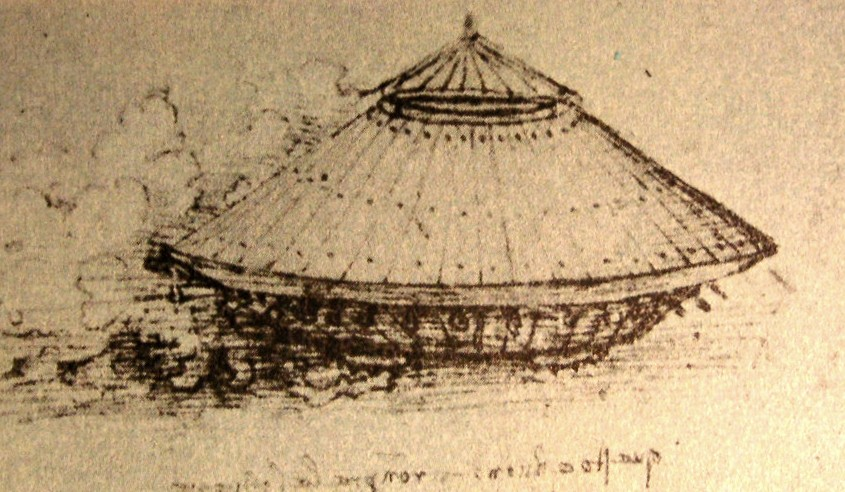
\includegraphics[scale=0.25]{imgs/Leonardo_tank.jpg}
 	\caption[Czołg Leonarda da Vinci]{\small{Szkic Leonarda da Vinci przedstawiający jego koncepcję czołgu.}\footnotemark}
	\label{czolg_leon}
    \end{center}
  \end{figure}
  \footnotetext{\emph{Czołg Leonarda da Vinci}, http://italoteka.blogspot.com,  (data dostępu 21.04.2015r.)}
Wiek XX niesie za sobą bardzo gwałtowny rozwój robotyki, który rozpoczął się w momencie skonstruowania w latach 40-tych pierwszego komputera. Ich rozwój był dodatkowo spotęgowany poprzez wybuch II wojny światowej i potrzebę łamania szyfrów dyplomatycznych.
W latach 50-tych wynaleziony został tranzystor, który aktualnie jest podstawowym elementem każdego urządzenia. Pozwolił on w znacznej mierze na zmniejszenie gabarytów komputerów (jednostek obliczeniowych), zmniejszenie zapotrzebowania na energię oraz wzrost mocy obliczeniowej co pozwoliło na konstrukcję autonomicznych robotów mobilnych.
Robotami mobilnymi nazywamy pojazdy, mogące zmieniać swoje położenie w przestrzeni. Dotyczy to nie tylko pojazdów jezdnych, ale także kroczących oraz latających. 
W 1956 r. ukończona została budowa elektrycznej wiewiórki\cite{robot_squee} (rysunek \ref{squee}), która posiadała dwa ,,zmysły": wzroku - zrealizowanego przy wykorzystaniu dwóch lamp fotoelektronowych oraz dotyku - dwóch krańcówek.  Napęd został zbudowany w oparciu o silniki elektryczne. Zwierzak, gdy zobaczył żołędzia (w tym przypadku jasno oświetlony punkt) kierował się w jego stronę, podnosił owoc przy pomocy ,,szufli" a następnie kierował się ,,do gniazda" - czyli miejsca, gdzie znajdowało się pulsacyjne źródło światła. Mimo ,iż realizowane zadanie jest bardzo proste to możemy mówić tutaj o pewnego rodzaju intelgencji ponieważ wiewiórka wykonywała pewną sekwencję ruchową bez interwencji człowieka ale w zależności od tego, co działo sie w jej otoczeniu.

  \begin{figure}[H]
    \begin{center}
      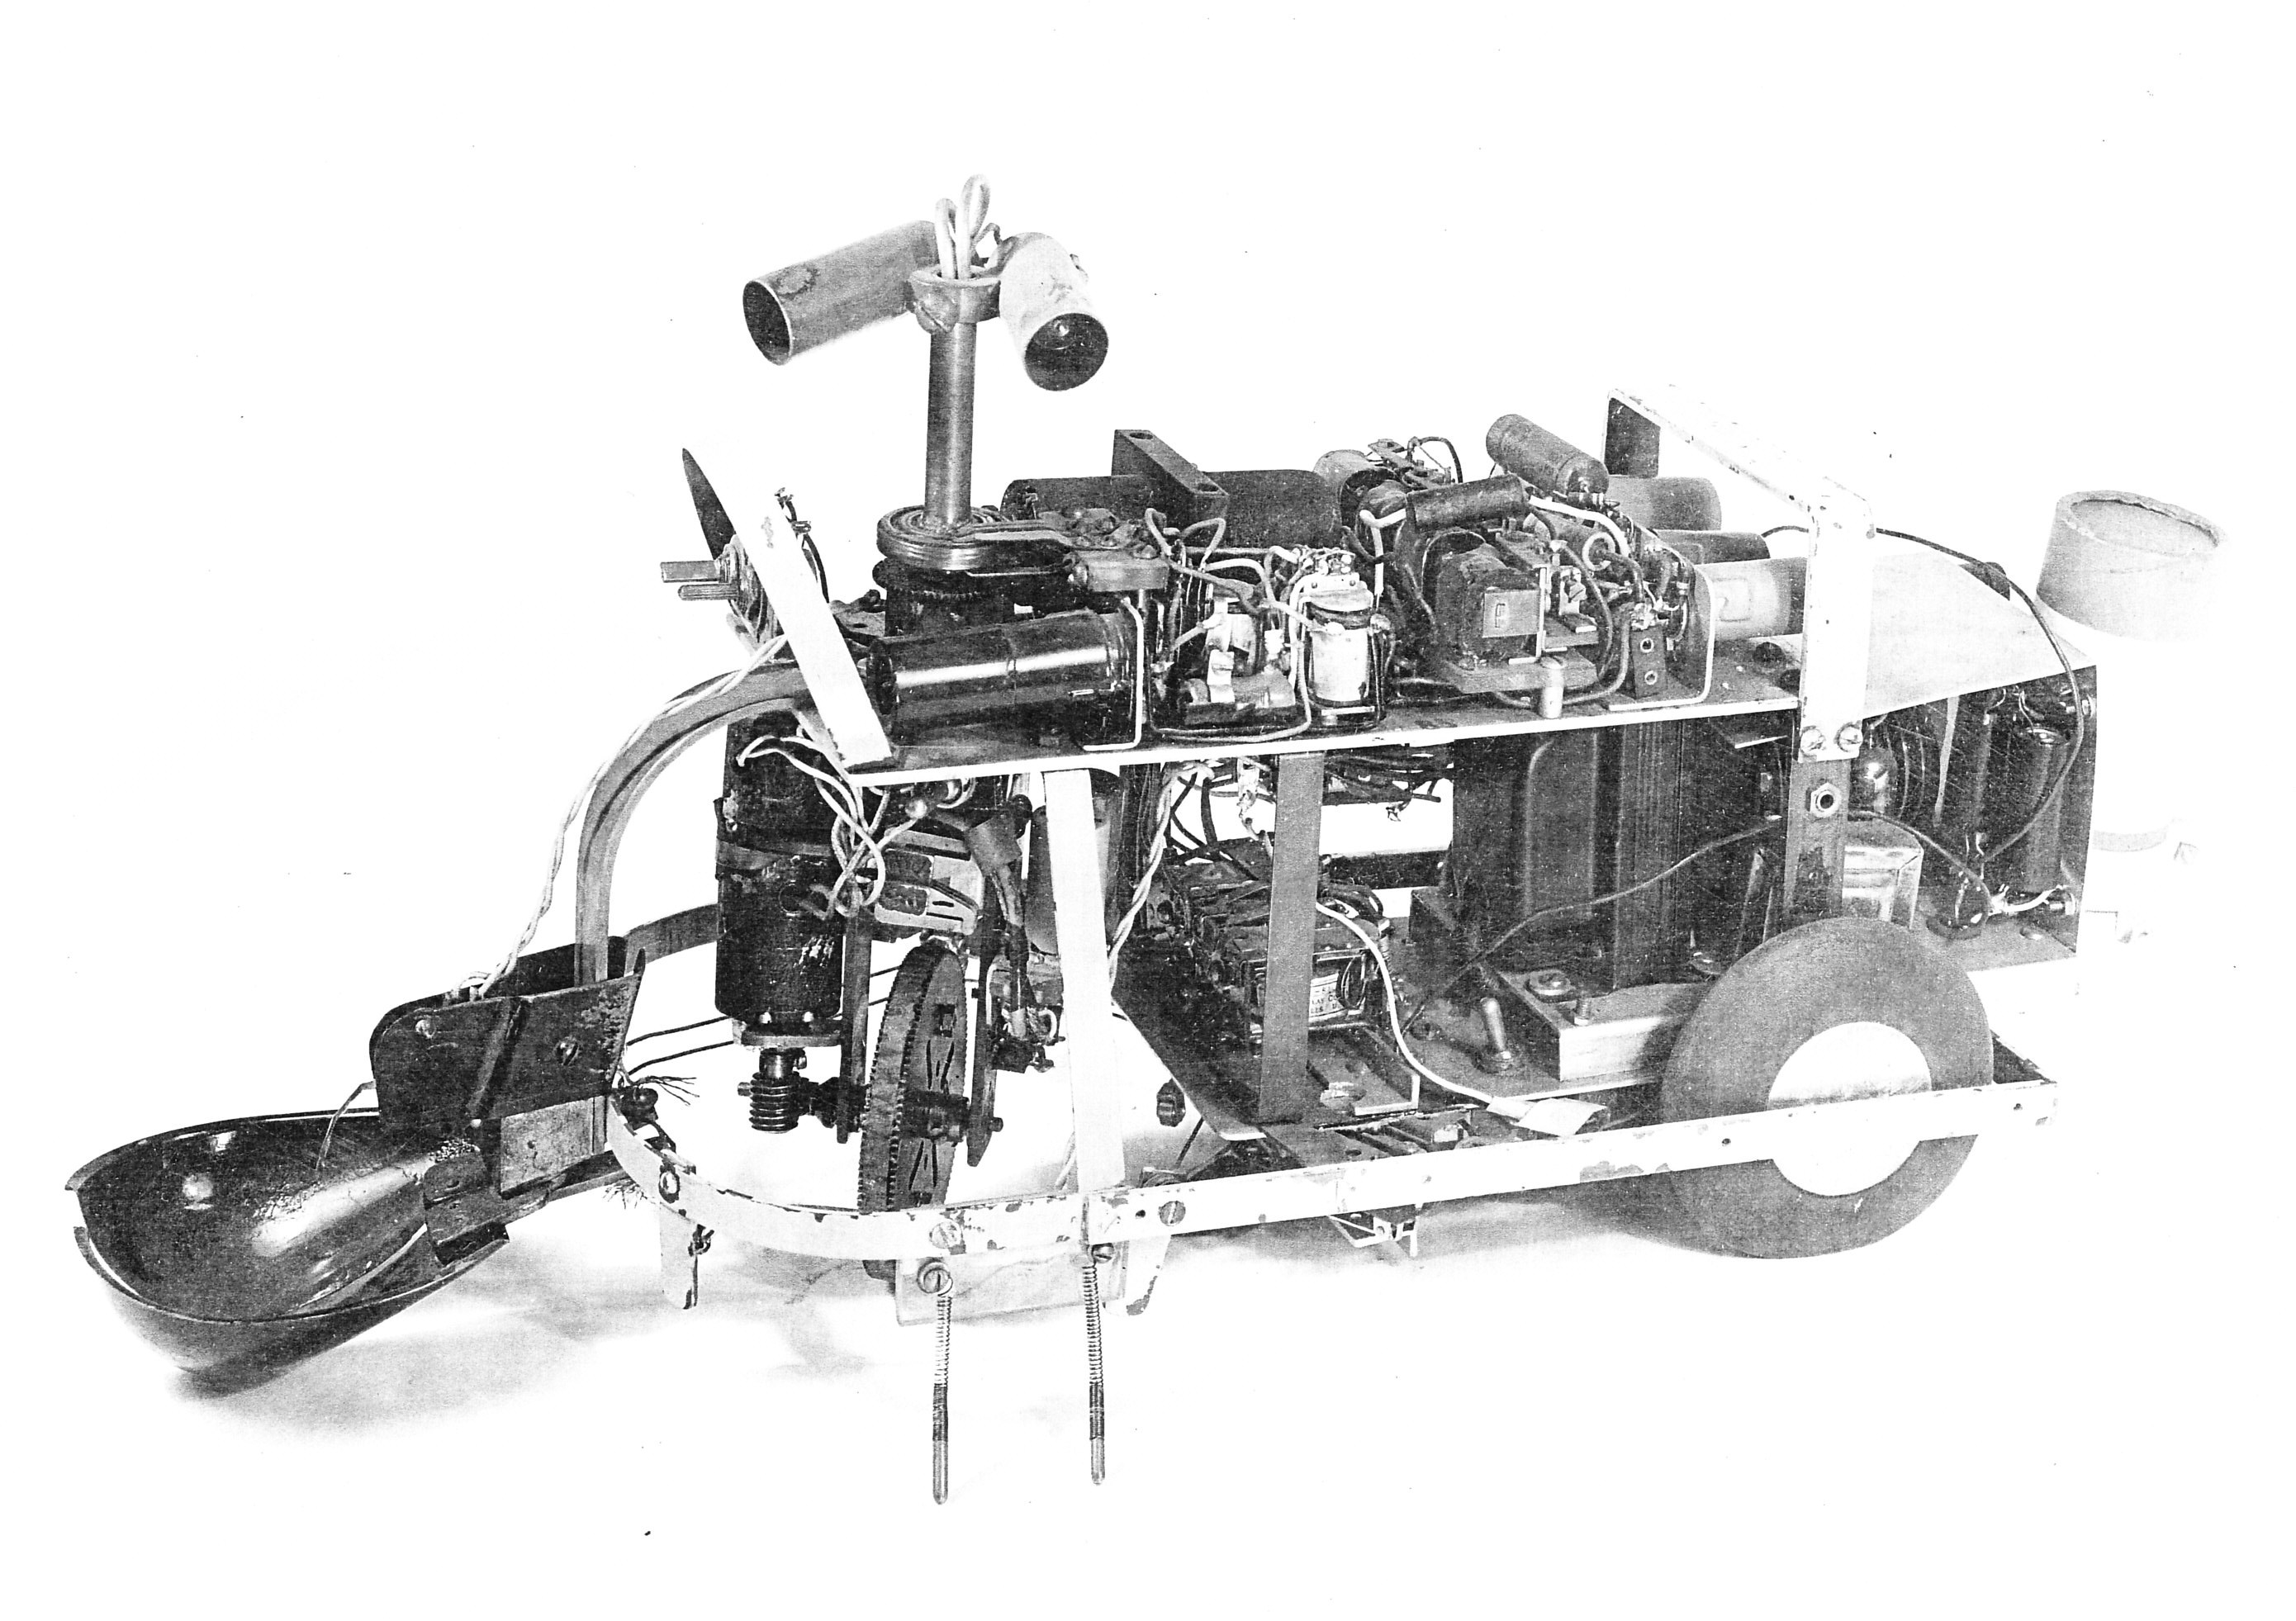
\includegraphics[scale=0.35]{imgs/Squee.jpg}
 \caption[Robot \textit{Squee}]{\small{Robot Squee zbudowany prze Jacka Koffa w 1959r.}\footnotemark}
        \label{squee}
    \end{center}
  \end{figure}
  \footnotetext{\emph{Robot Squee}, http://cyberneticzoo.com/,  (data dostępu 21.09.2015r.)}

Kolejne lata niosą za sobą coraz większą miniaturyzację wszelkich podzespów elektronicznych. Nie tylko zamykane są one w coraz mniejszych obudowach (pierwszy układ scalony - Jack St. Clair Kilby w 1958 r.) ale także charakteryzują się coraz wyższą sprawnością. Doprowadza to do tego, że pojazdy mobilne stają się obiektem zainteresowania służb specjalnych. W ten sposób w 1984 r. powstaje Prowler (rysunek \ref{state}) - pierwszy zdalnie sterowany robot o przeznaczeniu militarnym. Platforma ta mogła pełnić różne funkcje: od roli wsparcia - wyposażona w karabiny maszynowe, po funkcje rozpoznawcze - wyposażona w kamery.

  \begin{figure}[H]
    \begin{center}
      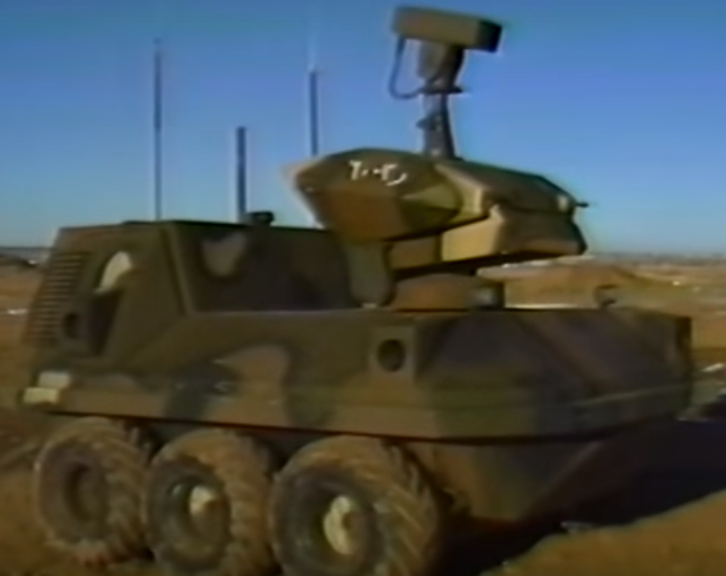
\includegraphics[scale=0.4]{imgs/state.png}
 \caption[Pojaz wojskowy \textit{Prowler}]{\small{Wojskowy robot mobilny Prowler .}\footnotemark}
        \label{state}
    \end{center}
  \end{figure}
  \footnotetext{\emph{Robot Defense Systems Prowler 1985}, https://youtube.com/,  (data dostępu 22.09.2015r.)}

Aktualnie najbardziej zaawansowanymi robotami mobilnymi są pojazdy wykorzystywane przez agencje kosmiczne do eksploracji kosmosu. Ich zaawansowana konstrukcja jest efektem bardzo rygorystycznych założeń jakie są im stawiane, tzn.: możliwie jak najmniejsze rozmiary, waga, wysoka mobilność oraz niezawodność, możliwość pracy w ciężkich, nieznanych warunkach środowiskowych. Na dodatek muszą one być zdolne do prowadzenia badań oraz zbierania próbek. Przykładem tej klasy robota może być marsjański łazik Curiosity Rover (rysunek \ref{lazik}).

  \begin{figure}[H]
    \begin{center}
      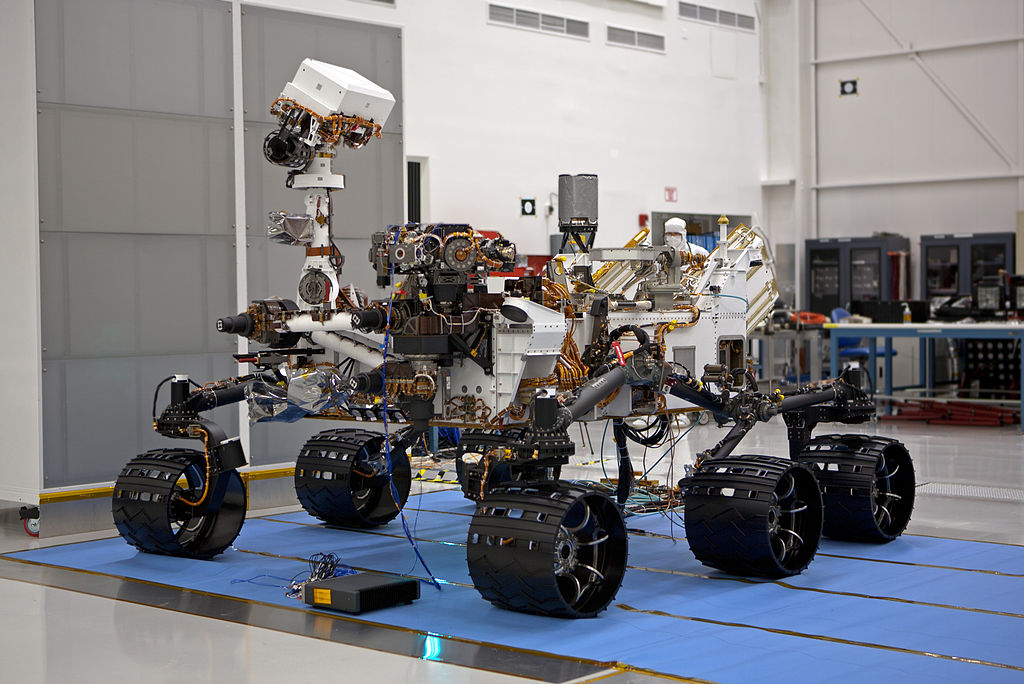
\includegraphics[scale=0.8]{imgs/curiosity.png}
 \caption[Łazik marsjański \textit{Curiosity}]{\small{Łazik marsjański Curiosity.}\footnotemark}
        \label{lazik}
    \end{center}
  \end{figure}
  \footnotetext{\emph{\textit{Curiosity}}, http://i.space.com/,  (data dostępu 22.09.2015r.)}

\chapter{Stan obecnej wiedzy}
\section{Rozw�j robotyki}
M�wi si� �e, �e robotyka jest owocem wszystkich dotychczasowych osi�gni�� ludzko�ci w ka�dej dziedzinie. ��czy w sobie przede wszystkim elementy : mechaniki, automatyki, elektroniki, sensoryki oraz cybernetyki.
Jej poszczeg�lne elementy by�y rozwijane na przestrzeni setek a nawet tysi�cy lat. Pierwsze wzmianki historyczne dotycz�ce budowy robot�w si�gaj� oko�o 350 roku p.n.e. i dotycz� greckiego matematyka Archtasa z Tarentu, kt�ry rzekomo zbudowa� ptaka nap�dzanego spr�onym powietrzem oraz potrafi�cego lata�. Niestety ale zweryfikowanie tej wiadomo�ci jest bardzo skomplikowane i nie daje jednoznacznej odpowiedzi. Wskazuje ona jednak na zainteresowanie ludzko�ci budow� maszyn-robot�w, kt�re pierwotnie mia�y na�ladowa� natur�. Za pocz�tek rozwoju robotyki uwa�a si� prze�om XV oraz XVI wieku, w kt�rym za spraw� wielkiego wynalazcy - Leonadra da Vinci powsta�o wiele interesuj�cych projekt�w oraz konstrukcji. Jego wizje niejednokrotnie znacznie wykracza�y poza czasy, w kt�rych �y�. Na ilustracji \ref{czolg_leon} przedstawiony zosta� szkic przedstawiaj�cych jedn� z zaprojektowanych przez Leonarda maszyn wojennych - przodek wsp�czesnego czo�gu, kt�ry mia� miota� kamienie oraz by� nap�dzany si�� ludzkich mi�ni.

\begin{figure}[h] \label{czolg_leon}
\centering
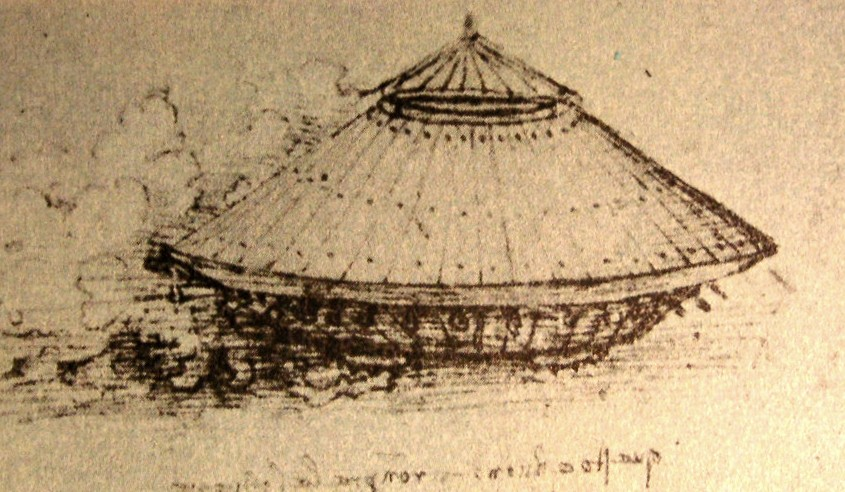
\includegraphics[scale=0.3]{imgs/Leonardo_tank.jpg}
\caption{Szkic Leonarda da Vinci przedstawiaj�cy jego koncepcj� czo�gu.}
\end{figure}

Kolejny prze�om w tej dziedzinie przypada na po�ow� XVIII wieku, w kt�rej to francuz Jacques de Vaucanson buduje swoje automaty. Z jego licznych konstrukcji pragn� wyr�ni� 3 najbardziej znane, tzn. : mechaniczny ch�opiec graj�cy na flecie, mechaniczny ch�opiec dodatkowo graj�cy na tamburynie, mechaniczn� kaczk�, potrafi�c� porusza� si�, wydawa� odg�osy, porusza� skrzyd�ami oraz symulowa� uk�ad trawienny.

Jednak�e prawdziwy prze�om w robotyce dokonuje si� w 1821 roku, w kt�rym Michael Faraday zbudowa� pierwszy silnik elektryczny, kt�rego dalszy rozw�j wywar� ogromny wp�yw na koncepcj� konstrukcji robot�w. Mechaniczne (np. spr�yny) oraz chemiczne (spalanie paliw) �r�d�a energii b�d� powoli wypierane z tej dziedziny nauki na rzecz rozwi�za� elektrycznych, pozwalaj�cych na prostsze, bezpieczniejsze oraz wydajniejsze magazynowanie oraz bardziej elastyczne wykorzystanie.

Upowszechnianie si� elektryczno�ci niesie za sob� szereg innych, znacz�cych wynalazk�w do jakich zaliczamy: wynalezienie przeka�nika elektrycznego przez Joseph'a Henry'ego w 1835 r., matematyczne zdefiniowanie przez George'a Bool'a zasad logiki, b�d�cej po dzie� dzisiejszy podstawowym narz�dziem matematycznym w teorii sterowania, konstrukcja zdalnie sterowanej �odzi skonstruowanej przez Nikola Tesl� w 1896 r.

Wiek XX niesie za sob� jeszcze gwa�towniejszy rozw�j tej dziedziny, kt�ry rozpocz�� si� w momencie skonstruowania w latach 40-tych pierwszego komputera. Ich rozw�j by� dodatkowo spot�gowany poprzez wybuch II wojny �wiatowej oraz potrzeb� �amania szyfr�w dyplomatycznych. W latach 50-tych wynaleziony zosta� tranzystor, kt�ry aktualnie jest podstawowym elementem ka�dego urz�dzenia. Pozwoli� on w znacznej mierze na zmniejszenie gabaryt�w komputer�w (jednostek obliczeniowych), zmniejszenie zapotrzebowania na energi� oraz wzrost mocy obliczeniowej co pozwoli�o na konstrukcj� autonomicznych robot�w mobilnych.

\section{Historia czo�gu}
Od zarania dziej�w za wojnami kry� si� najszybszy oraz najgwa�towniejszy rozw�j technologiczny. Rozw�j cywilizacyjny nast�puje nieco p�niej, poniewa� ka�da nowa technologia (jak np. GPS czy Internet) najpierw wprowadzana jest na potrzeby wojska a dopiero w p�niejszych latach wprowadzana jest do u�ytku dla ludno�ci cywilnej. Podobnie mia�a si� sytuacja z I wojn� �wiatow� - konflikt ten da� pocz�tek m.in. bojowym pojazdom opancerzonym, kt�re otrzyma�y nazw� czo�g�w.

I wojna �wiatowa by�a jednym z najwi�kszych konflikt�w zbrojnych w dziejach ludzko�ci, kt�ry walkami ogarn�� niemal�e ca�� Europ�. Do jej wybuchu przyczyni�a si� nie tylko sytuacja polityczna ale tak�e nastroje panuj�ce w�wczas w spo�ecze�stwie, kt�re "chcia�o wojny". I Wojna �wiatowa niew�tpliwie na zawsze odmieni�a pola walki. Jeszcze przed jej rozpocz�ciem nast�pi� intensywny rozw�j broni maszynowej - jednym z pierwszych, w pe�ni sprawnych, karabin�w maszynowych by�a tak zwana kartaczownica Gatlinga, skonstruowana ju� w 1861 roku. Jednak dopiero podczas I wojny �wiatowej bro� maszynowa rozpowszechni�a si� na tyle, �eby diametralnie zmieni� oblicze pola walki. Linie obronne zosta�y g�sto obsadzone ci�kimi karabinami maszynowymi, takimi jak brytyjski Vickers czy wiele wersji karabin�w Maxima, kt�re osi�ga�y praktyczn� szybkostrzelno�� na poziomie 500-600 pocisk�w na minut� oraz zasi�g przekraczaj�cy kilometr. Z kolei oddzia�y piechoty otrzyma�y bro� l�ejsz� (np. francuski r�czny karabin maszynowy Chauchat czy brytyjski lekki karabin Lewis), kt�ra, mimo gorszych parametr�w od wspomnianych wcze�niej konstrukcji, by�a rewolucyjn� zmian� na tle karabin�w powtarzalnych, b�d�cych do tej pory jedyn� broni� piechoty. I wojna �wiatowa by�a konfliktem, w kt�rym atakuj�ca piechota by�a zasypywana, zbieraj�cym �miertelne �niwo, gradem pocisk�w. W efekcie tego morale �o�nierzy bardzo szybko podupad�o i nie chcieli oni ju� gin�� w imi� wy�szo�ci racji politycznych. Konflikt przekszta�ci� si� w wojn� pozycyjn�, w kt�rej piechota wi�cej czasu sp�dza�a w okopach ni� walcz�c. Wszelkie znane metody walki zawodzi�y w tej nowej sytuacji: atak kawalerii mia�a jeszcze mniejsze szanse powodzenia ni� piechoty, a stosowane na wielk� skal� nawa�y artyleryjskie nie by�y w stanie wystarcz�co zmi�kczy� linii obronnych.
Aby wygra� wojn� nale�a�o w jaki� spos�b dosta� si� bli�ej przeciwnika.


W celu przedarcia si� przez "ziemi� niczyj�" czyli stref� pomi�dzy okopami skonstruowano g�sienicowy pojazd opancerzony. Zadaniem pierwotnym czo�g�w by� jedynie bezpieczny transport. Przyk�adem tego typu pojazd�w jest przedstawiony na ilustracji \ref{czolg_ws} pojazd \textit{Mark I} ,kt�rego specjalnie uformowane g�sienice (w kszta�t r�wnoleg�oboku) pozwala�y �atwiej pokonywa� zasieki wroga. 

\begin{figure}[h] \label{czolg_ws}
\centering
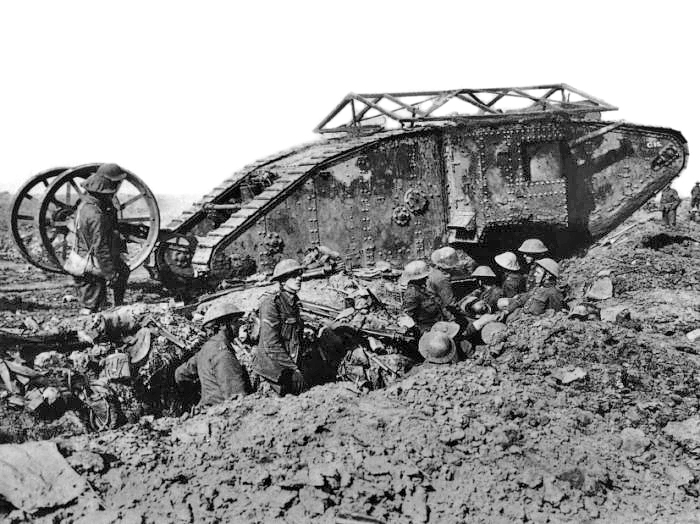
\includegraphics[scale=0.3]{imgs/ws_czolg.jpg}
\caption{Czo�g Mark I u�yty pierwszy raz w bitwie pod Somm� w 1916 r.}
\end{figure}

\begin{figure}[h] \label{czolg_ws}
\centering
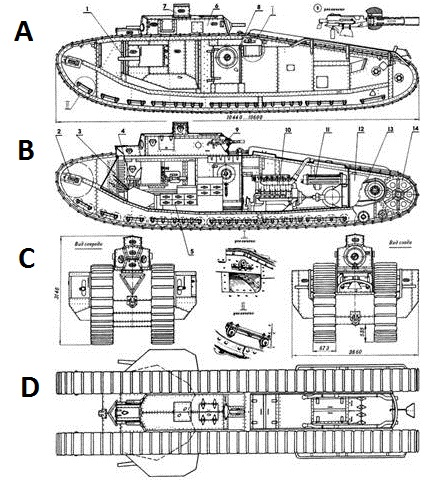
\includegraphics[scale=0.3]{imgs/markviii.jpg}
\caption{Unowocze�niona wersja }
\end{figure}

Zastosowanie czo�g�w pozwoli�o na szybkie zako�czenie konfliktu. Jednak�e pocz�tkowo nie wszyscy dostrzegli w tych pojazdach potencja� militarny. Wynika�o to z faktu, �e by�y one bardzo powolne i s�abo uzbrojone - o niewielkiej warto�ci bojowej. Pocz�tkowo, skoro tylko wojska alianckie posiada�y czo�gi, nie by�o potrzeby montowania w nich wielkiego dzia�a gdy� by�y one przeznaczone do zwalczania piechoty. 

Po zako�czeniu dzia�a� zbrojnych prawie wszystkie pa�stwa przyst�pi�y do projektowania w�asnych pojazd�w bojowych. Zacz�to zatem bra� pod uwag� mo�liwo�� walk typu czo�g-czo�g (a nie jak w przypadku I W� jedynie czo�g-piechota). Efektem tego by�o tworzenie czo�g�w o mo�liwe dobrym pancerzu oraz dziale. Pierwsze konstrukcje tzw. czo�g�w lekkich pojawi�y si� w okolicy 1930 r. Przyk�adem takiego pojazdu mo�e by� radziecki T-26

 

Zosta�y one rozwijane oraz modernizowane. Pocz�tkowo wozy te walczy�y jedynie z piechot� oraz artyleri�. Podczas II wojny �wiatowej dochodzi�o ju� do walk typu czo�g-czo�g co wymusi�o na konstruktorach wyposa�enie ich w pot�ne armaty zdolne do zniszczenia przeciwnika. 

\section{Roboty mobilne}

Robotami mobilnymi nazywamy pojazdy, mog�ce zmienia� swoje po�o�enie w przestrzeni. Dotyczy to nie tylko pojazd�w jezdnych, ale tak�e krocz�cych oraz lataj�cych. Ich g��wn� zalet� jest to ,�e mo�emy nimi sterowa� na odleg�o��. Pozwala to doprowadzi� je do miejsc ,kt�re dla cz�owieka s� niedost�pne lub wykonywa� zadania w �rodowisku zagra�aj�cym naszemu �yciu. Maszyny te s� aktualnie szeroko wykorzystywane przez~:
\begin{itemize}
\item  
s�u�by specjalnie np. wojsko, gdzie mog� pe�ni� rol� bezza�ogowych pojazd�w bojowych lub szpiegowskich,
\item 
agencje kosmiczne, gdzie prowadz� badania badania na innych cia�ach niebieskich (np. eksploracja Marsa przez �azik Curiosity Rover),
\item 
ratownictwo medyczne, gdzie rozwa�a si� wprowadzenie robot�w lataj�cych (typu quadrocopter) do szybkiego dostarczenia pierwszej pomocy w przypadku ataku serca,
\item
geolog�w oraz meteorolog�w do zdalnego dokonywania pomiar�w.
\end{itemize}

\begin{figure}[h]
\centering
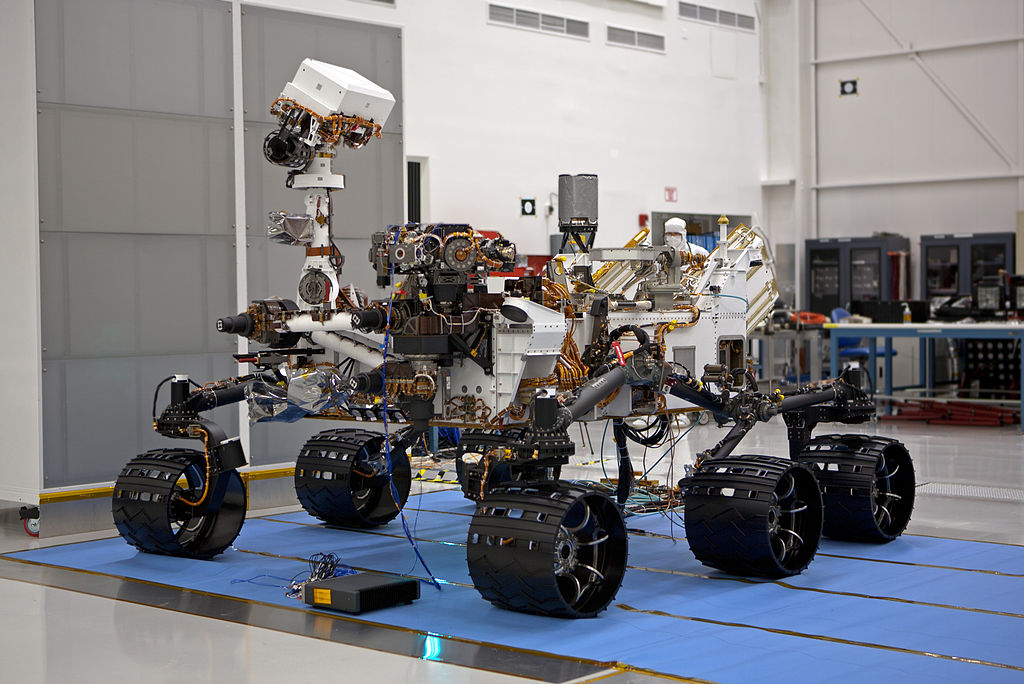
\includegraphics{imgs/curiosity.png}
\caption{Zdj�cie �azika Curiosity Rover jeszcze przed wys�aniem w kosmos.}
\end{figure}

Omawiane maszyny mo�emy dodatkowo wyposa�y� w inteligentne algorytmy pozwalaj�ce na autonomiczn�, czyli pozbawion� wp�ywu cz�owieka, prac�. Dzi�ki wykorzystaniu czujnik�w pomiarowych oraz przy pomocy odpowiedniego oprogramowania mog� one samoistnie rozwi�zywa� niekt�re, z g�ry za�o�one, zadania.

\namedchapter[Adam Zieliński]{Konstrukcja mechaniczna}
Proces budowy robota rozpoczął się od stworzenia trójwymiarowego modelu pojazdu. Projekt wykonany został przy wykorzystaniu studenckiej wersji oprogramowania Autodesk Inventor Professional 2014. Symulacja 3D miała na celu przede wszystkim ukazanie złożoności całego projektu. Pozwoliła m.in. na dokładne rozmieszczenie wszystkich komponentów wraz z uwzględnionymi rzeczywistymi wymiarami. Na rysunku \ref{mod3d} przedstawiony został uzyskany efekt wraz z naniesionymi oznaczeniami poszczególnych elementów. 

  \begin{figure}[H]
    \begin{center}
      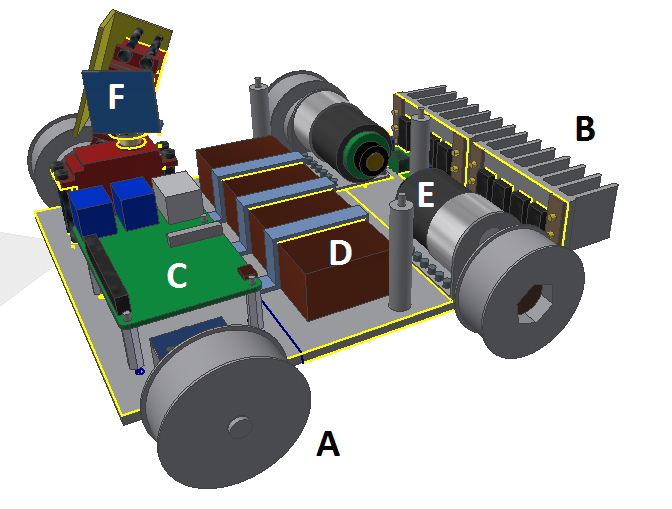
\includegraphics[scale=0.65]{imgs/calosc_2.png}
 	\caption[Model 3D projektowanego czołgu.]{\small{Model 3D projektowanego pojazdu. A - koła, B - mostki H wraz z radiatorami, C - Raspberry 2 Pi Model B, D - bateria, E - silniki prądu stałego, F - wieżyczka}}
	\label{mod3d}
    \end{center}
  \end{figure}
\namedsection{Podstawa pojazdu}
Wszystkie elementy zgrupowane na rysunku \ref{mod3d} tworzą korpus pojazdu, który został osadzony na sklejce brzozowej o grubości 5 mm. Materiał został wybrany pod kątem łatwości w obróbce oraz trwałości. Ze względu na jego warstwową strukturę jest on bardzo wytrzymały i jednocześnie bardzo lekki. Wyżej omówiony model pozwolił jednoznacznie dobrać wymiary podstawy oraz bardzo dokładnie wskazać miejsca, w których należało wykonać otwory mocujące dla poszczególnych komponentów. 

  \begin{figure}[H]
    \begin{center}
      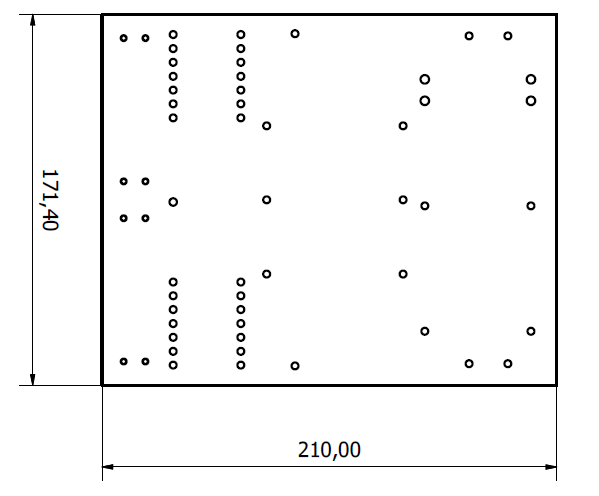
\includegraphics[scale=0.5]{imgs/podstawa.png}
 	\caption[Podstawa pojazdu.]{\small{Podstawa pojazdu wraz z naniesionymi wymiarami w milimetrach i otworami niezbędnymi do zamocowania poszczególnych elementów.}}
	\label{podst3d}
    \end{center}
  \end{figure}
\namedsection{Wieżyczka}
Wieża pojazdu zbudowana została w oparciu o 2 serwa modelarskie TowerPro SG-5010. Serwomechanizmy są zintegrowanymi układami elektronicznymi zawierającymi sekcję mechaniczną (silnik wraz z przekładnią) oraz układ sterowania położeniem.
Na rysunku \ref{wieza3d} przedstawiono model omawianego segmentu. Serwo A jest zamocowane bezpośrednio do podstawy pojazdu i dzięki niemu realizowany jest obrót prawo/lewo wieży. Do orczyka, czyli obrotowej części mechanizmu, zamocowane zostało mocowanie serwa B, które zostało wykonane z aluminiowego kątownika. Jest to materiał, który bardzo dobrze nadaje się do tego typu rozwiązań ponieważ jest tani, łatwo dostępny, lekki i stosunkowo wytrzymały.  

  \begin{figure}[H]
    \begin{center}
      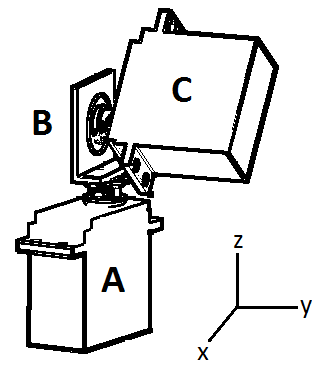
\includegraphics[scale=0.45]{imgs/wieza_3d.png}
 	\caption[Model wieżyczki.]{\small{Trójwymiarowy model konstrukcji wieżyczki robota. A - serwomechanizm odpowiedzialny za obrót wokół osi OZ, B - serwomechanizm obrotu w osi OY, C - łączenie pomiędzy elementami.}}
	\label{wieza3d}
    \end{center}
  \end{figure}
\namedsection{Napęd}
W projekcie wykorzystano dwa szczotkowe silniki prądu stałego Pololu 37Dx52L wraz z przekładnią 30:1. Dla napięcia 12 V pojedynczy silnik wytwarza moment obrotowy wynoszący 8 kg$\cdot$cm i obraca się z prędkością 350 obrotów na minutę. Rysunek techniczny przedstawiający dokładne wymiary wykorzystanego silnika przedstawiono na rysunku \ref{wymiary_silnika}. Maksymalny pobór prądu (przy zatrzymaniu wału) może wynieść około 5 A.

  \begin{figure}[H]
    \begin{center}
      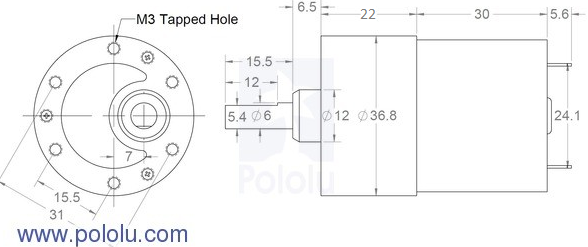
\includegraphics[scale=0.7]{imgs/silnik_wymiary.png}
 	\caption[Wymiary silnika Pololu 37Dx52L ]{\small{Wymiary wykorzystanego silnika - Pololu 37Dx52L }\footnotemark}
	\label{wymiary_silnika}
    \end{center}
  \end{figure}
  \footnotetext{http://pololu.com/, (data dostępu 20.10.2015r.)}

Jednym z założeń było zastosowanie w pojeździe napędu gąsienicowego. Robot zbudowany został w oparciu o 4 aluminiowe koła metryczne 27T5/32 - koła pasowe stosowane w przemyśle do przełożenia napędu. Ich średnica to 54 mm. Razem z dedykowanym pasem zębatym T5 o długości 420 mm tworzą układ gąsienic. Na ilustracji \ref{gasienice_elementy} przedstawione zostały wykorzystane elementy.

  \begin{figure}[H]
    \begin{center}
      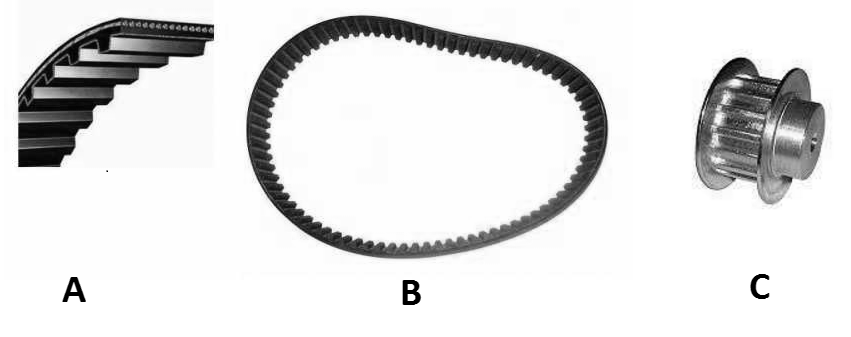
\includegraphics[scale=0.5]{imgs/gasienice.png}
 	\caption[Elementy gąsienic.]{\small{Rysunki A i B przedstawiają pas zębaty T5, C - koło zębate T5. }\footnotemark}
	\label{gasienice_elementy}
    \end{center}
  \end{figure}
  \footnotetext{http://centrum-cnc.pl/, (data dostępu 29.10.2015r.)}

Wybrane koła metryczne posiadały na środku otwór o średnicy 8 mm, podczas gdy oś silników ma średnicę 6 mm. Należało zatem wykonać mocowanie, pozwalające na sztywne osadzenie kół na wale. Do tego celu wykorzystano otrzymane wraz z silnikami sześciokątne nakładki, przedstawione na rysunku \ref{zamocowanie_szesciokatne}. Wycięcie otworu w kształcie sześciokąta w warunkach domowych jest bardzo trudne. W związku z tym, dzięki projektowi w środowisku CAD, możliwe było zlecenie wykonania go firmie zewnętrznej, specjalizującej się w cięciu wodą pod wysokim ciśnieniem.

  \begin{figure}[H]
    \begin{center}
      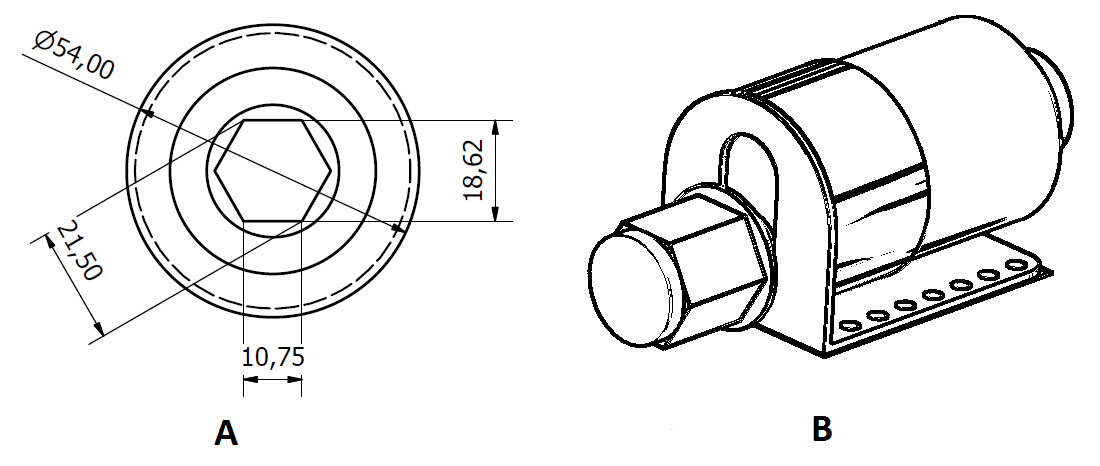
\includegraphics[scale=0.40]{imgs/moc_kol_tyl.png}
 	\caption[Model tylnych kół.]{\small{Na ilustracji znajduje się rysunek techniczny koła metrycznego(A) dostosowanego na potrzeby mocowania na silniku z wykorzystaniem sześciokątnej przejściówki(B).}}
	\label{zamocowanie_szesciokatne}
    \end{center}
  \end{figure}

Podczas tworzenia projektu należało także rozważyć sposób mocowania przednich kół. Ze względu na fakt, iż gąsienice (prawa/lewa) mogą obracać się jednocześnie w dwóch rożnych kierunkach, należało zastosować osobną oś dla prawego oraz lewego koła. Jej model przedstawiony został na rysunku \ref{zamocowanie_przod}. Element A wykonany został z drewna dębowego, które jest bardzo twarde i pozwala na dokładne spasowanie z osią B, wykonaną z aluminium.

  \begin{figure}[H]
    \begin{center}
      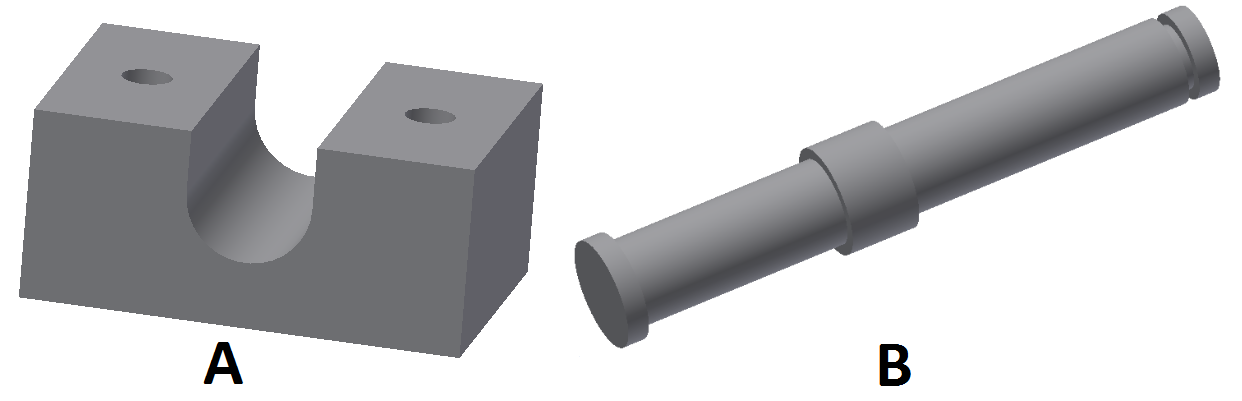
\includegraphics[scale=0.40]{imgs/moc_kol_prz.png}
 	\caption[Model mocowania kół przednich.]{\small{Na rysunku przedstawiony został model mocowań kół przednich pojazdu. A - przedstawia blok łączący oś B z podstawą robota.}}
	\label{zamocowanie_przod}
    \end{center}
  \end{figure}
  \newpage
\namedsection{Efekt końcowy}
Wykonanie oraz ostateczne dopasowanie wszystkich elementów było dość czasochłonne. Należy jednak wspomnieć o tym, że dzięki wykonaniu trójwymiarowego modelu czas ten niewątpliwie uległ znacznemu skróceniu. Końcowy efekt, wraz z zamocowaniem części elektronicznej przedstawiony został na zdjęciu poniżej (rys. \ref{czolg_calosc}).
  \begin{figure}[H]
    \begin{center}
      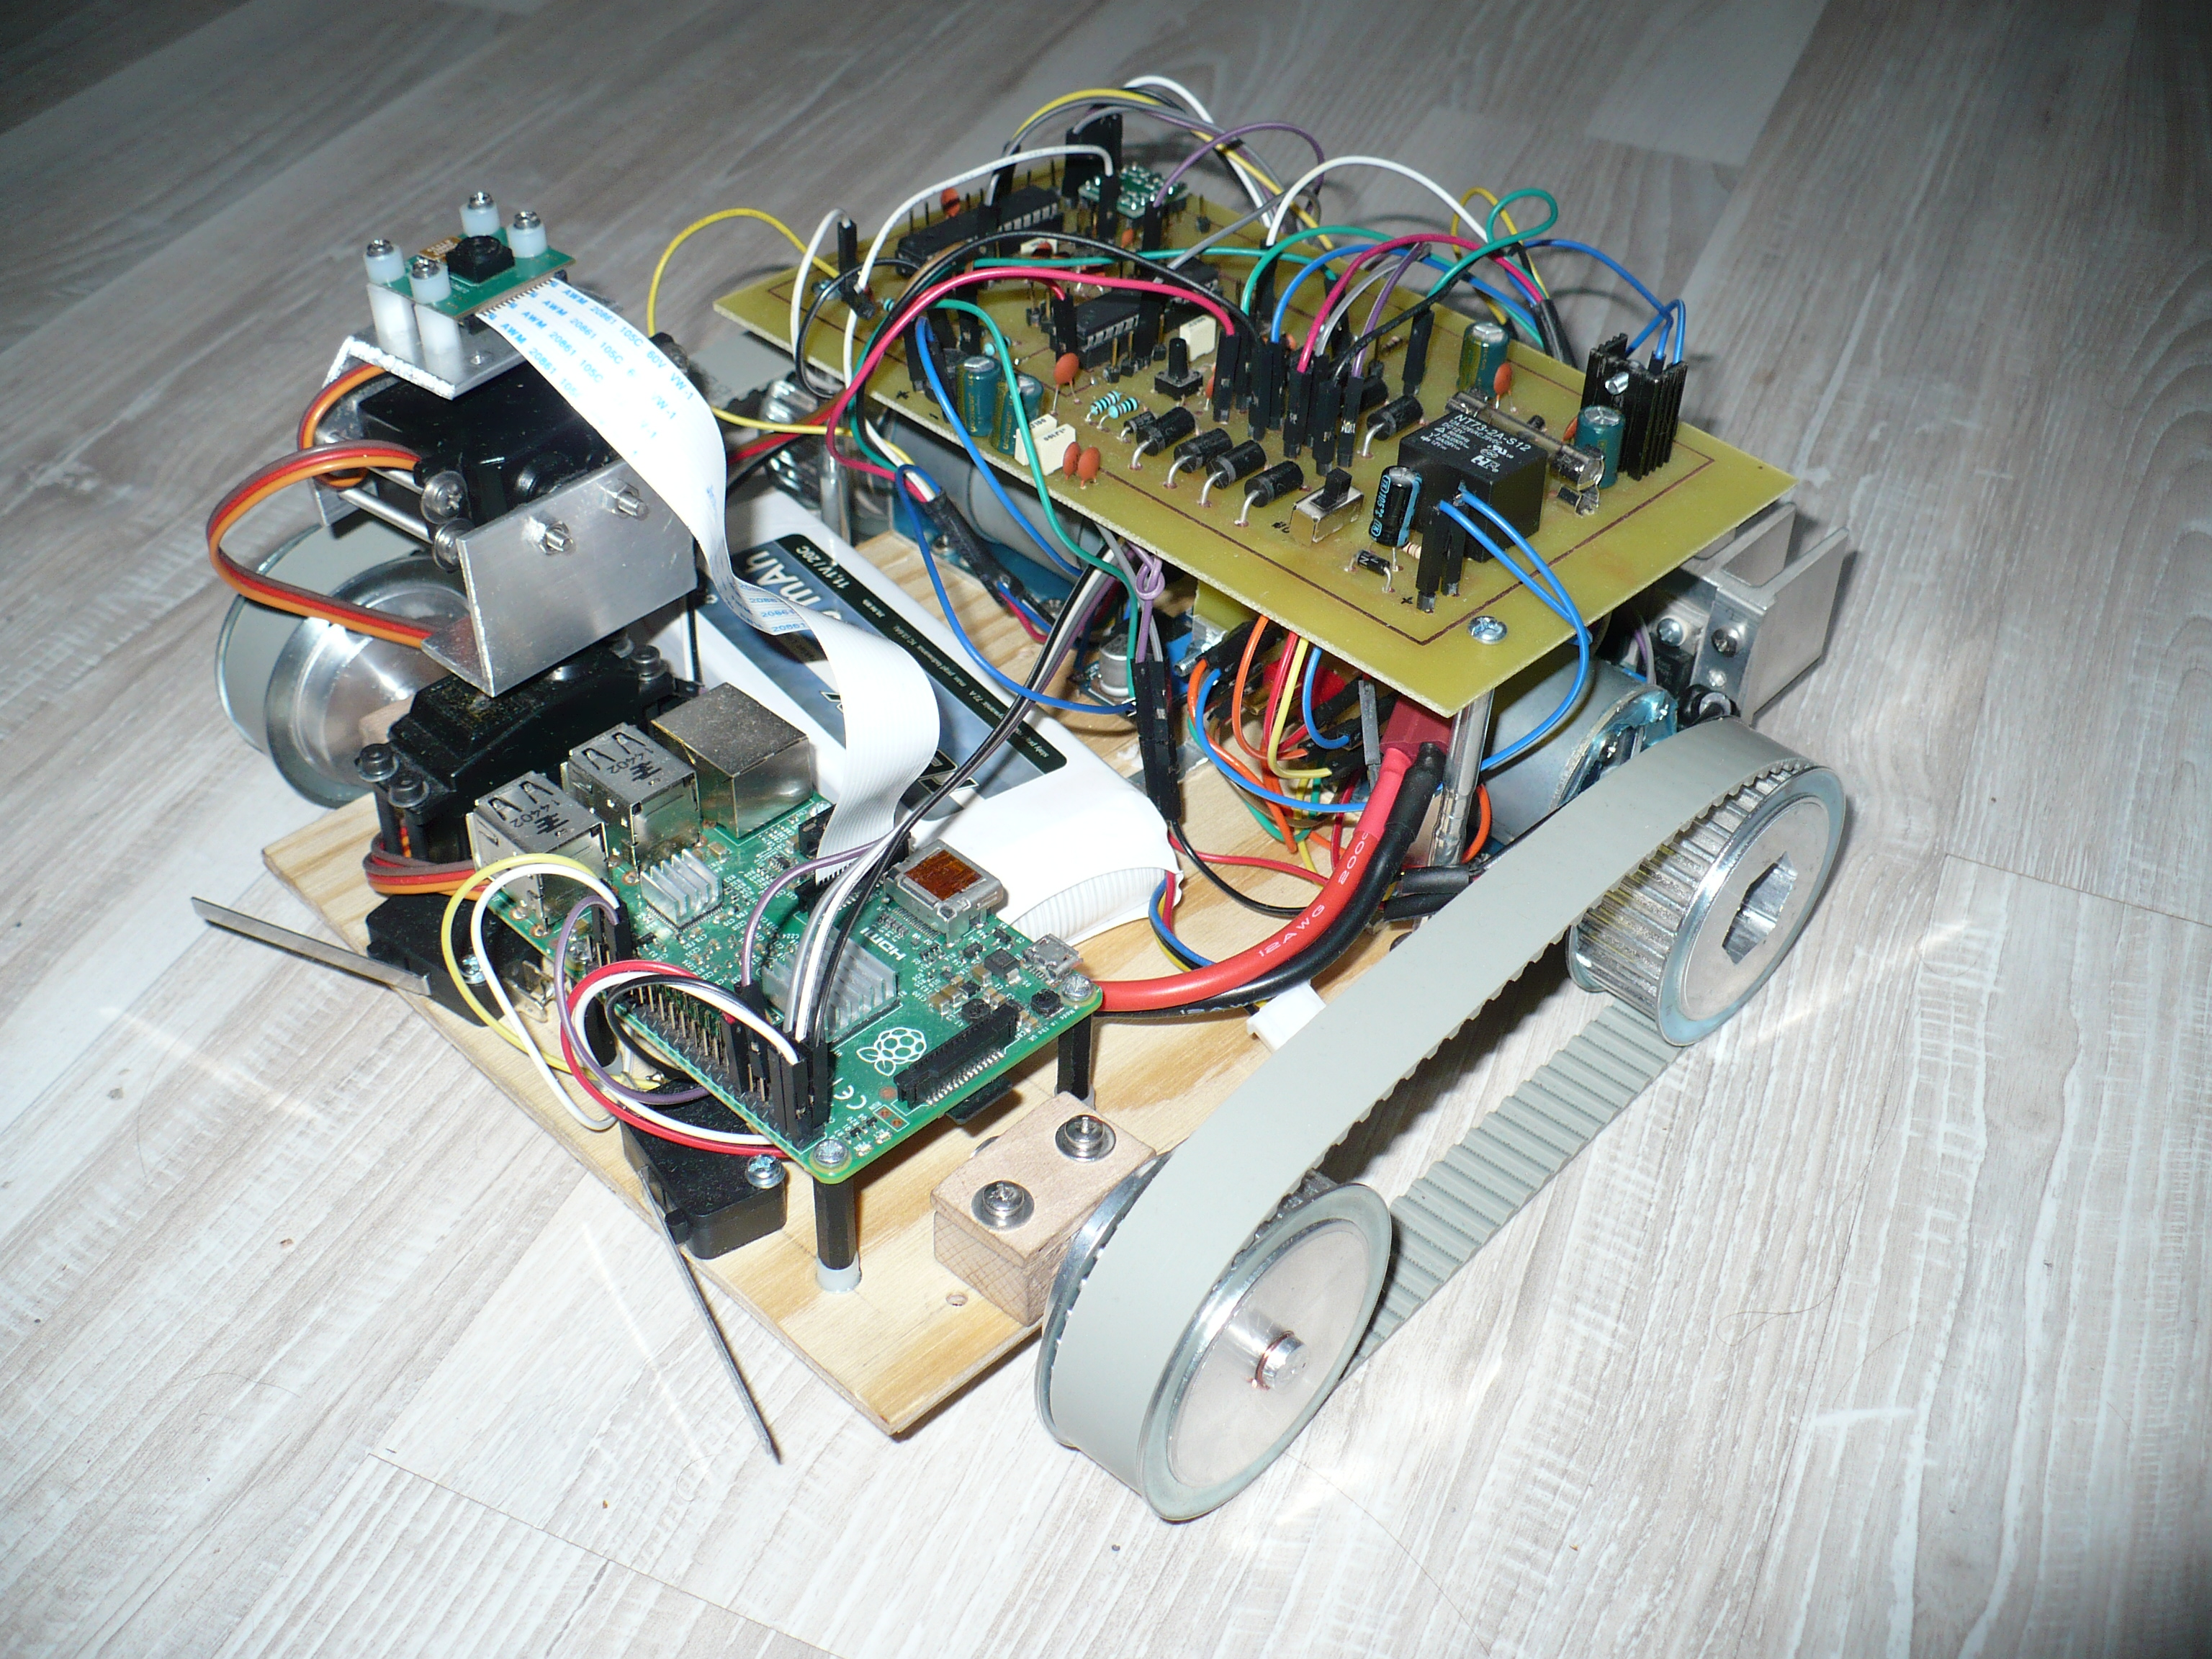
\includegraphics[scale=0.13]{imgs/czolg.jpg}
 	\caption[Zbudowany model.]{\small{Zdjęcie przedstawia kompletny robot typu czołg. Jest to całkowicie wykonany model wraz z częścią elektroniczną.}}
	\label{czolg_calosc}
    \end{center}
  \end{figure}

\namedchapter[Adam Zieliński]{Projekt elektroniki}
Podstawowym zadaniem projektu jest budowa robota mobilnego, na którą składa się część mechaniczna, elektroniczna oraz programowa. Pierwsza z nich została omówiona w poprzednim rozdziale. Następnym krokiem jest zaprojektowanie oraz wykonanie części wykonawczej, która pozwoli połączyć platformę \textit{Raspberry Pi} z rzeczywistym modelem i umożliwi sterowanie nim. 
\namedsection{Założenia}
Sterowanie pojazdem odbywa się poprzez wykorzystanie dwóch silników \textit{Pololu 37Dx52L} oraz dwóch serwomechanizmów \textit{TowerPro SG-5010}. Każdy z nich sterowany jest przy pomocy sygnału PWM (ang. \textit{Pulse-Width Modulation}), czyli sygnału prostokątnego o zmiennym współczynniku wypełnienia, co zostało pokazane na rysunku \ref{sygnal_PWM}. Aby jak najbardziej zoptymalizować proces sterowania należało wykorzystać sprzętowe generatory sygnału PWM. W odróżnieniu od programowych rozwiązań, nie obciąża to pracy procesora. Jest to o tyle istotne ,iż głównym zadaniem czołgu jest analiza obrazu pochodzącego z kamery w czasie rzeczywistym, co jest bardzo czasochłonnym procesem. Wybrana platforma \textit{Raspberry Pi} posiada dwa sprzętowe kanały PWM, z czego jeden przeznaczony jest do generowania sygnału audio. Z pojedynczego źródła możliwe jest wytworzenie dwóch przebiegów, o tej samej częstotliwości lecz różnym wypełnieniu, które posłużą do sterowania położeniem wieżyczki. Sterowanie silnikami napędowymi wymaga użycia jeszcze dodatkowo czterech sygnałów PWM. W związku z czym zaprojektowany został osobny układ elektroniczny, który pozwolił na ich obsługę. Zbudowany został w oparciu o dwa mikrokontrolery z rodziny AVR, łączące się przy pomocy magistrali szeregowej magistrali TWI(ang. \textit{2-wire Serial Interface}) z \textit{Raspberry Pi}. Komunikacja z robotem będzie wykorzystać sieć WLAN(ang. \textit{Wireless Local Area Network,}) oraz protokoł SSH (ang. \textit{secure shell}). Schemat blokowy elektroniki czołgu przedstawiony został na rysunku poniżej:

  \begin{figure}[H]
    \begin{center}
      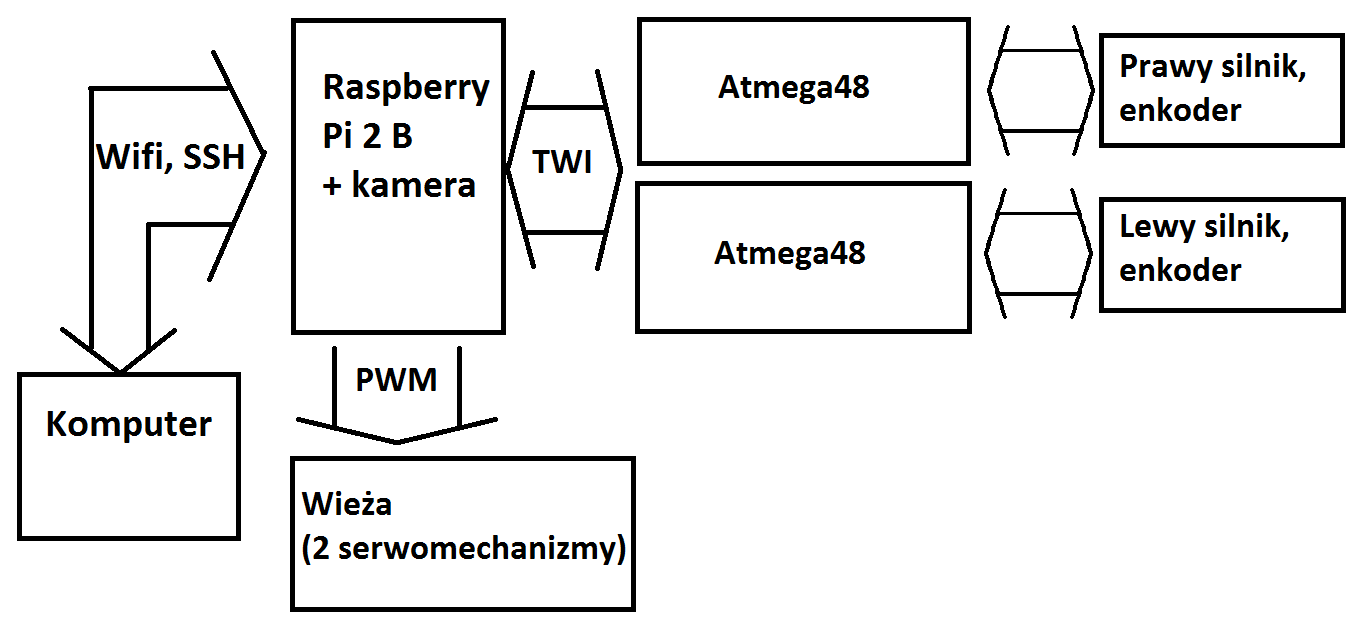
\includegraphics[scale=0.35]{imgs/idea.png}
 	\caption[Koncepcja elektroniki.]{\small{Ogólna koncepcja elektroniki pojazdu.}}
	\label{sygnal_PWM}
    \end{center}
  \end{figure}  
  
\namedsection{Raspberry Pi}
\textit{Raspberry Pi 2 model B} jest w minikomputerem zbudowanym w oparciu o procesor ARM Cortex-A7. Wyposażony jest w 4 porty USB (ang. \textit{Universal Serial Bus}) oraz port HDMI (ang. \textit{High Definition Multimedia Interface}) co pozwala na podłączenie monitora, klawiatury oraz myszki i czyni go w pełni funkcjonalnym komputerem. Dodatkowo istnieje możliwość zainstalowania na jego pokładzie specjalnej odmiany systemu Linux - Raspbiana, która jest zoptymalizowana i dostosowana do uwarunkowań sprzętowych \textit{Raspberry Pi}. Pozwala ona obsługę urządzenia przy pomocy wiersza poleceń oraz graficznego interfejsu użytkownika. Omawiane urządzenie łączy w sobie uniwersalność komputera klasy PC oraz mikrokontrolera. Płytka wyposażona jest w 40 pinów ogólnego przeznaczenia zapewniających m.in. komunikację TWI, generowanie sygnałów PWM czy dowolna programowa obsługa pozostałych wejść/wyjść. System operacyjny dodatkowo zawiera w sobie narzędzia niezbędne do pisania programów wykorzystujących jego sprzętowe zasoby zarówno w języku C++ jak i Pythonie. 

\begin{figure}[H]
    \begin{center}
      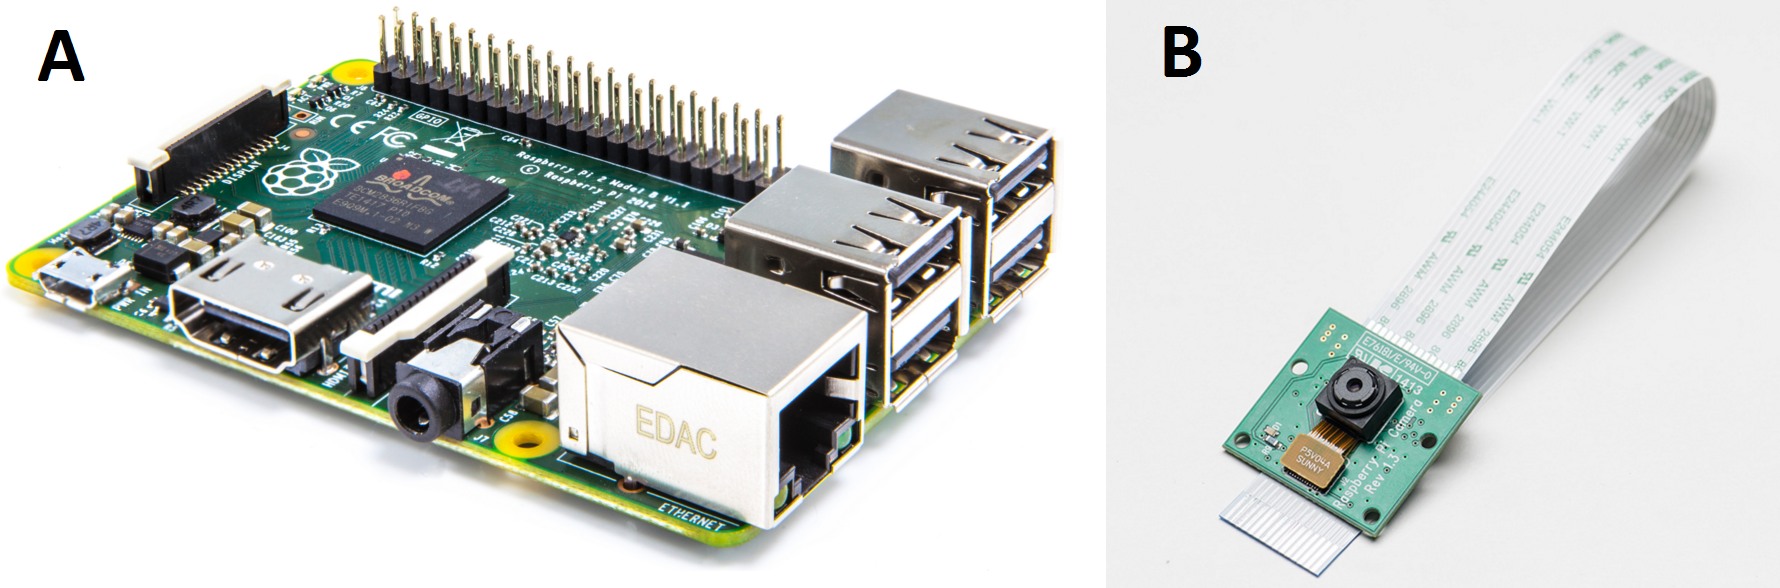
\includegraphics[scale=0.3]{imgs/raspberry_pi.png}
 	\caption[Raspberry Pi wraz z kamerą.]{\small{Na zdjęciu przedstawione zostało: A - \textit{Raspberry 2 Pi Model B}}\footnotemark \small{, B - dedykowana kamera \textit{Raspberry Pi Camera HD}}\footnotemark }
	\label{trans_TWI}
    \end{center}
  \end{figure}  
  	  \footnotetext[1]{\emph{Pi2ModB1GB}, http://raspberrypi.org/,  (data dostępu 27.12.2015 r.)}
  	  \footnotetext{\emph{RaspberryPi camera}, http://parallella.org/,  (data dostępu 27.12.2015 r.)}

Realizowany projekt inżynierski wykorzystuje wspomniany układ do realizacji analizy obrazu, które pozyskiwane są przez dedykowaną kamerę - \textit{Raspberry Pi Camera HD}. Kamera łączy się z minikomputerem przy wykorzystaniu interfejsu CSI (ang. \textit{Camera Serial Interface}) prowadzonego przy pomocy 15-pinowej taśmy. Tym co odróżnia CSI od innych popularnych interfejsów szeregowych (np. USB) jest to, że zapewnia większą przepustowość danych. Wykorzystana tutaj komunikacja składa się z: interfejsu I$^2$C, którym przesyłane są sygnały sterujące pracą kamery, dwóch dodatkowych szyn danych przeznaczonych do przesyłania obrazu oraz synchronizującej je szyny zegarowej. 
Budowany pojazd jest robotem mobilnym, co uniemożliwia podłączenie do niego monitora oraz klawiatury na stałe. Istnieje jednak możliwość w pełni funkcjonalnej, zdalnej łączności z textit{Raspberry Pi} z poziomu komputera osobistego. Do tego calu należy wyposażyć minikomputer w adapter WLAN, aby mógł połączyć się z bezprzewodową siecią lokalną do której podłączony jest także komputer osobisty. Raspbian umożliwia obsługę protokołu SSH  czyli realizację połączenia typu serwer-klient, do której obsługi wystarczy jedynie znajomość adresu IP (ang. \textit{Internet Protocol Address}) \textit{Raspberry}.
  
\namedsection{Sterowanie napędem}
Do napędzenia pojazdu użyte zostały szczotkowe silniki prądu stałego firmy Pololu, których ideowa konstrukcja została pokazana poniżej (rys. \ref{silnik_p}). Obrót wału silnika spowodowany jest wystąpieniem siły elektromotorycznej $F$, czyli siły działającej na przewód o długości $L$, przez który płynie prąd $I$, znajdujący się w polu magnetycznym o indukcji $B$ definiowanej jako:
\begin{equation}
	F =  BIL
   \label{eq:sila_elektromotoryczna}
 \end{equation}
 gdzie:  
 \begin{equationDescriptor}
   \EQDitem{$F$}{siła [N],}
 	\EQDitem{$B$}{indukcja magnetyczna [T],}
 	 \EQDitem{$I$}{natężenie prądu [A],}
 	  \EQDitem{$L$}{długość przewodu [m].}
 \end{equationDescriptor}
 \newpage
  \begin{figure}[H]
    \begin{center}
      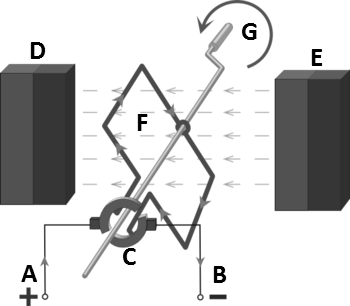
\includegraphics[scale=0.7]{imgs/silnik_p_stalego.png}
 	\caption[Schemat ideowy silnika prądu stałego.]{\small{Rysunek przedstawia ideową budowę szczotkowego silnika prądu stałego, którym możemy wskazać jego poszczególne elementy: A i B - zaciski zasilania, są źródłem prądu płynącego przez ramkę F umieszczoną w polu magnetycznym wytworzonym przez dwa magnesy stałe D i E. Ramka zamocowana jest do osi obrotowej silnika E oraz łączy się z komutatorem C, który jest odpowiedzialny za zmianę kierunku przepływu prądu poprzez zmianę polaryzacji napięcia.}\footnotemark}
	\label{silnik_p}
    \end{center}
  \end{figure}  
  	  \footnotetext{\emph{Silnik prądu stałego}, http://wiki.wolnepodreczniki.pl/,  (data dostępu 28.12.2015 r.)}
\noindent
Sterowanie silnikami odbywa się poprzez zmianę wartości siły $F$. Indukcję magnetyczną $B$ oraz długość przewodu $L$ przyjmuje się jako wartości stałe. Zatem jedynym parametrem, dzięki któremu możliwa jest jej regulacja jest prąd $I$. Dodatkowo zakładając ,że rezystancja ramek wirnika jest zawsze taka sama oraz prawo Ohma (wzór \ref{eq:prawo_ohma}) regulacja upraszcza się do zmiany wartości napięcia zasilającego~$U$. 
\begin{equation}
	I = \frac{U}{R}
   \label{eq:prawo_ohma}
 \end{equation}
 gdzie:  
 \begin{equationDescriptor}
   \EQDitem{$U$}{napięcie [V],}
 	\EQDitem{$R$}{rezystancja [$\Omega$],}
 	 \EQDitem{$I$}{prąd [A],}
 \end{equationDescriptor}
\noindent
Do tego celu wykorzystany został tzw. sygnał PWM, czyli sygnał prostokątny o zmiennym wypełnieniu i określonej częstotliwości (rys. \ref{sygnal_PWM}), którą można obliczyć ze wzoru:
\begin{equation}
	f =  \frac{1}{T}
   \label{eq:czestotliwosc}
 \end{equation}
 gdzie:  
 \begin{equationDescriptor}
   \EQDitem{$f$}{częstotliwość [Hz],}
 	\EQDitem{$T$}{okres sygnału [s].}
 \end{equationDescriptor}
\noindent
 Wypełnienie sygnału definiujemy jako stosunek czasu trwania sygnału do okresu:
 \begin{equation}
	k =  \frac{dT}{T} \cdot 100\%
   \label{eq:wsp_wypelnienia}
 \end{equation}
 gdzie:  
 \begin{equationDescriptor}
   \EQDitem{$dT$}{czas trwania niezerowej wartości sygnału [s],}
 	\EQDitem{$T$}{okres sygnału [s],}
 	\EQDitem{$k$}{współczynnik wypełnienia [\%].}
 \end{equationDescriptor}
 \newpage
  \begin{figure}[H]
    \begin{center}
      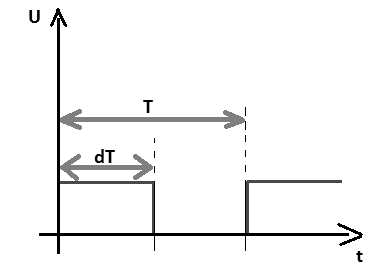
\includegraphics[scale=0.65]{imgs/wykres.png}
 	\caption[Sygnał PWM.]{\small{Na wykresie przedstawiony został przykładowy przebieg PWM, czyli fala prostokątna o okresie $T$ oraz czasie trwania sygnału $dT$.}}
	\label{sygnal_PWM}
    \end{center}
  \end{figure}  
  \noindent
  Wartość wypadkowego napięcia możemy obliczyć ze wzoru:
  \begin{equation}
	U_{sk}=\sqrt{\frac{1}{T}\int\limits_{0}^{dT}u(t)^2dt}
   \label{eq:napiecie_skuteczne}
 \end{equation}
 gdzie:  
 \begin{equationDescriptor}
   \EQDitem{$U_{sk}$}{napięcie skuteczne [V],}
 	\EQDitem{$T$}{okres sygnału [s],}
 	 \EQDitem{$dT$}{czas trwania niezerowej wartości sygnału [s].}
 \end{equationDescriptor}
 
 \namedsection{Sterowanie wieżyczką}
Serwomechanizm jest kompaktowym urządzeniem mechaniczno-elektronicznym (rys. \ref{serwomechanizm}) składającym się z silnika prądu stałego oraz sterownika. Najczęściej układy tego typu realizują sterowanie położeniem wału wyjściowego i mają ograniczony zakres pracy (np. umożliwiają obrót o 270$^\circ$). Urządzenia posiadają w sobie pętlę sprzężenia zwrotnego (np. przy wykorzystaniu potencjometru połączonego z wałem) oraz zaimplementowany sterownik. 
  \begin{figure}[H]
    \begin{center}
      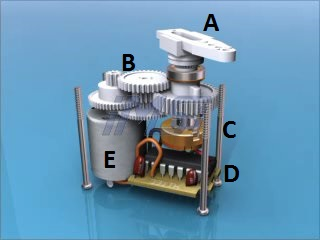
\includegraphics[scale=0.8]{imgs/serwo.jpg}
 	\caption[Model sewomechanizmu.]{\small{Ilustracja przedstawia wewnętrzną budowę serwomechanizmu, na którym: A - orczyk, czyli część obrotowa/wykonawcza, B - zespół kół zębatych redukujących prędkość obrotową, C - potencjometr realizujący sprzężenie zwrotne od położenia orczyka, D - układ elektroniczny będący sterownikiem układu, E - silnik prądu stałego.}\footnotemark}
	\label{serwomechanizm}
    \end{center}
  \end{figure}  
  	  \footnotetext{\emph{Model serwomechanizmu}, http://imsi.pl/,  (data dostępu 28.12.2015r.)}
\noindent
Sterowanie, podobnie jak w przypadku napędu, odbywa się przy wykorzystaniu modulacji szerokości impulsu PWM. Jednakże generowany sygnał musi mieć określoną częstotliwość - 50 Hz a zmiana wypełnienia powoduje zmianę położenia orczyka. Przykładowy sposób sterowania przedstawiony został na rysunku \ref{serwomechanizm_sterowanie}. Dla wypełnienia $k=7,5$\% układ ustawia się w położeniu neutralnym, czyli w połowie zakresu działa - 90$^\circ$ względem początkowego położenia. Zmniejszając stopniowo wypełnienie sygnału sterującego orczyk będzie zmniejszał kąt wychylenia (aż dojdzie do 0 $^\circ$), zwiększając - kąt będzie narastał aż do 180$^\circ$.
\begin{figure}[H]
    \begin{center}
      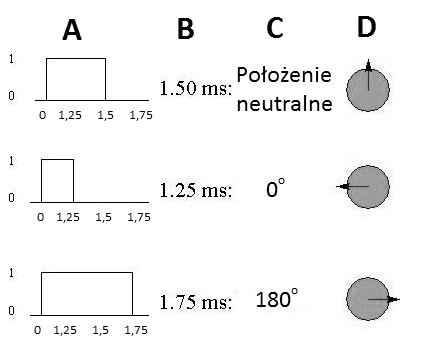
\includegraphics[scale=0.8]{imgs/ster_serw.png}
 	\caption[Sterowanie serwomechanizmem.]{\small{Ilustracja przedstawia przykładowe sterowanie serwomechanizmem. Kolumna A przedstawia sygnał wejściowy o częstotliwości 50 Hz, czyli okresie $T=20$ ms, B - wskazuje nam czas trwania sygnału $dT$, C i D - położenie wału wyjściowego.}\footnotemark}
	\label{serwomechanizm_sterowanie}
    \end{center}
  \end{figure}  
  	  \footnotetext{\emph{Co to jest serwomechanizm?}, http://henryk.mbapp.com/,  (data dostępu 28.12.2015r.)}
  	  
\namedsection{Magistrala TWI}
Interfejs TWI jest protokołem komunikacyjnym pozwalającym połączyć ze sobą różnego rodzaju układy elektroniczne takie jak mikrokontrolery czy czujniki pomiarowe. Dane przesyłane są szeregowo z wykorzystaniem dwóch linii sygnałowych: SCL (ang. \textit{Serial Clock Line}) oraz SDA (ang. \textit{Serial Data Line}). Do funkcjonowania magistrali nie są wymagane żadne układy zewnętrzne. Należy jedynie zapewnić wysoki stan logicznego (5 V lub 3,3 V) na szynach, co przedstawione zostało na rysunku \ref{podlaczenie_TWI}. Dodatkowo każde z podłączonych urządzeń musi posiadać swój unikalny adres. Wartości rezystorów R1 oraz R2 są odwrotnie proporcjonalne do pojemności pasożytniczej magistrali oraz prędkości przesyłu danych.
\begin{figure}[H]
    \begin{center}
      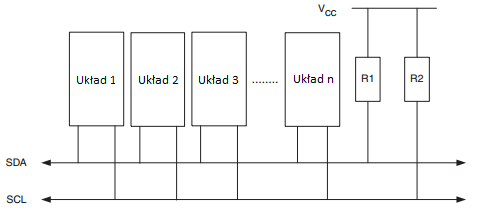
\includegraphics[scale=0.9]{imgs/magistrala_twi.png}
 	\caption[Magistrala TWI.]{\small{Rysunek przedstawia sposób podłączenia urządzeń do wspólnej magistrali TWI. Wymagane jest dołączenie rezystorów podciągających R1 dla SDA i R2 dla SCL dla zapewnienia wysokiego stanu logicznego linii.}\footnotemark}
	\label{podlaczenie_TWI}
    \end{center}
  \end{figure}  
  	  \footnotetext{\emph{Atmega48 datasheet}, http://atmel.com/,  (data dostępu 20.08.2015 r.)}
\newpage
\noindent
Urządzenia mogą pracować w dwóch trybach :
\begin{table}[h!tb]
\centering
\small
\caption{Tryby pracy TWI}
\begin{tabularx}{\linewidth}[c]{|l|X|} 
\hline
	Tryb & Pełniona funkcja \\ \hline
 	\textit{Master} & Urządzenie nadrzędne, może inicjować transmisję, jest odpowiedzialny za generowanie sygnału zegarowego.  \\ \hline
 	\textit{Slave} & Nie może inicjować wymiany danych. Transmisja możliwa jest jedynie w odpowiedzi na sygnał otrzymany od urządzenia typu \textit{Master}, nie może generować sygnału zegarowego.\\ \hline
 	\noalign{\smallskip}
\end{tabularx}
\vspace{-8pt}
\end{table}
\newline
\noindent
Przykładowa wymiana informacji pomiędzy układem \textit{Master} i \textit{Slave} została przedstawiona na rysunku \ref{trans_TWI}. W stanie bezczynności każda z szyn danych ma wysoki stan logiczny. Inicjacja transmisji rozpoczyna się wysłaniem tzw. bitu startu - \ref{trans_TWI}A, czyli wymuszeniem zbocza opadającego linii danych gdy linia zegarowa utrzymuje stan wysoki. Następnie \textit{Master} szeregowo wysyła bajt danych, z czego najstarsze 7 bitów to adres urządzenia docelowego - \ref{trans_TWI}B (stąd do magistrali można podłączyć maksymalnie $2^7$ urządzeń). Najmłodszy bit oznacza realizowaną funkcję : 0 - zapis, 1 - odczyt - \ref{trans_TWI}C. Urządzenie, które poprawnie odczytało swój unikalny adres powinno w odpowiedzi wygenerować bit potwierdzenia - \ref{trans_TWI}D. Następnie rozpoczyna się transmisja danych - \ref{trans_TWI}E. Dane wysyłane są bajtami. Każda odebrana ramka potwierdzana jest bitem potwierdzenia~-~\ref{trans_TWI}F. Transmisja nie definiuje ilości możliwych do wysłania bitów. Trwa ona tak długo, aż nie pojawi się bit stopu, czyli zbocze narastające na linii SDA w momencie ,gdy SCL ma stan wysoki - \ref{trans_TWI}G. Mimo możliwości podłączenia do 128 urządzeń nie możliwe jest prowadzenie wielu transmisji jednocześnie. Największą zaletą TWI jest możliwość podłączenia względnie dużej ilości układów przy wykorzystaniu jedynie dwóch pinów mikrokontrolera. 
\begin{figure}[H]
    \begin{center}
      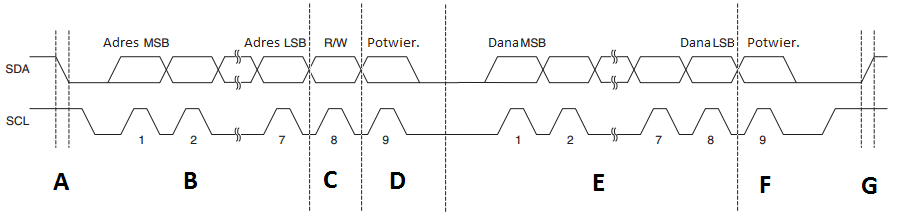
\includegraphics[scale=0.6]{imgs/transmisja_twi.png}
 	\caption[Transmisja TWI.]{\small{Rysunek przedstawia przykładową transmisję danych. Kolejne etapy to: A - bit startu (\textit{Master}), B - wysłanie adresu urządzenia docelowego (\textit{Master}), C - bit oznaczający zapis/odczyt danych (\textit{Master}), D - bit potwierdzenia odbioru generowany przez urządzenie docelowe (\textit{Slave}), E - bajt danych (zapis - \textit{Master} lub odczyt - \textit{Slave}) , F - potwierdzenie odbioru (zapis - \textit{Slave} lub odczyt - \textit{Master}), G - bit stopu (\textit{Master}). MSB (ang. \textit{Most Significant Bit}) - najbardziej znaczący bit, LSB (ang. \textit{Least Significant Bit}) - najmniej znaczący bit. }\footnotemark}
	\label{trans_TWI}
    \end{center}
  \end{figure}  
  	  \footnotetext{\emph{Atmega48 datasheet}, http://atmel.com/,  (data dostępu 20.08.2015 r.)}	
  	  
\namedsection{Sterownik silników}
Silniki napędowe wyposażone są w enkodery impulsowe, czyli  urządzenia które generują (w tym przypadku) około 370 impulsów na jeden, pełny obrót koła. Jest to wystarczające źródło informacji, na podstawie którego można określić prędkość obrotu silnika a następnie zaprojektować regulator prędkości. Sterownik zrealizowany jest przy wykorzystaniu  mikrokontrolerów z rodziny AVR, Atmega48. Jest to 8-bitowy układ oparty na architekturze RISC (ang. \textit{Reduced Instruction Set Computing} – polega on przede wszystkim na uproszczeniu listy rozkazów, składającej się w większości z poleceń wykonywanych w jednym takcie zegara, co umożliwia szybsze wykonywanie kodu) oraz architekturze harwardzkiej, w której to pamięć danych programu jest oddzielona od pamięci rozkazów. Jednostka ta jest wyposażona w sprzętowe generatory sygnałów PWM oraz liczniki pozwalające zliczać sygnały z enkoderów - co w pełni spełnia nasze wymagania. Dodatkowo układy AVR wspierają także komunikację wykorzystującą protokół TWI - co zapewnia nam pełną integrację z \textit{Raspberry Pi}.

\namedsection{Zasilanie}
Aby projektowany pojazd był w pełni mobilny należy wyposażyć go w baterię. Powinna ona charakteryzować się stosunkowo dużą pojemnością, niewielkimi wymiarami, niewielką masą,napięciem pracy do 12 V oraz dużą wydajnością prądową. Uwzględniając przedstawione wymagania wybrany został 3-ogniwowy akumulator litowo-polimerowy (LiPo) o pojemności 3600 mAh oraz wydajności prądowej 20C. Pojedyncze ogniwo generuje napięcie około 3,7 V. Zastosowana bateria jest pakietem złożonym z trzech, szeregowo połączonych ogniw, dzięki czemu wyjściowe napięcie wynosi $3\cdot3,7$ V$ = 11,1$ V. Wydajność prądowa określona jako 20C informuje, że maksymalny prąd, który nie spowoduje uszkodzenia baterii, wynosi $20\cdot3600$ mAh$=72$ A. Bardzo istotnym elementem dotyczącym prawidłowej obsługi pakietu jest zapewnienie jej odpowiedniego prądu ładowania, który powinien wynosić maksymalnie około 1C. Podczas eksploatacji baterii należy zwrócić szczególną uwagę na napięcia wyjściowe każdego ogniwa. Przesadne rozładowanie któregokolwiek z nich prowadzi do nieodwracalnego uszkodzenia całego pakietu. W związku z tym do ich ładowania stosuje się specjalnie skonstruowane ładowarki pozwalające na kontrolowanie napięcia każdego ogniwa z osobna.

\namedchapter[Adam Zieliński]{Schemat elektroniki}
Schemat elektroniki oraz projekt płytki drukowanej wykonany został przy wykorzystaniu środowiska Altium Designer. Program pozwala narysować schemat ideowy układu oraz na jego podstawie zaplanować rozmieszczenie komponentów i miedzianych ścieżek na laminacie. Dodatkowo umożliwia ręczne tworzenie bibliotek elementów elektronicznych wraz z uwzględnieniem ich rzeczywistych rozmiarów. Schemat ideowy przedstawia zależności pomiędzy poszczególnymi układami wchodzącymi w skład projektowanego urządzenia, co ma celu zaprezentowanie całości w sposób przyjazny dla konstruktora. Powstała struktura nie musi odzwierciedlać rzeczywistych odległości oraz faktycznego rozłożenia komponentów. W związku z tym dopiero na jego podstawie tworzy się projekt płytki drukowanej, na którego podstawie wykonany zostanie rzeczywisty układ.
\namedsection{Zasilanie} 
Do prawidłowego funkcjonowania robota wymagana jest realizacja kilku poziomów napięcia, dokładniej: 12 V dla silników napędowych oraz 5 V dla układów logicznych. Silniki napędowe sterowane będą przy wykorzystaniu sygnału PWM mikrokontrolera. Jest to sygnał sterujący o amplitudzie 5 V (takiej jak napięcie zasilania) oraz  niewielkiej wydajności prądowej (rzędu kilkudziesięciu mA) co całkowicie dyskwalifikuje go jako bezpośrednie źródło zasilającego. Dodatkowo w dokumentacji technicznej zastosowanych silników napędowych (Pololu 37Dx52L) widnieje informacja, że dla napięcia 12 V oraz w przypadku zatrzymania wału mogą pobrać prąd o wartości dochodzącej do 5 A. W związku z tym należy wykorzystać tzw. mostek H, którego zadaniem jest wykorzystanie sygnału sterującego do nasycenia tranzystorów mocy, które mogą przepuszczać znacznie większe prądy. Jego realizacja została przedstawiona na rysunku \ref{mostek_h_sch}. Jest to projekt AVT 1756, który ukazał się w czasopiśmie Elektronika Praktyczna. Złącza Vcc oraz GND podłączone są bezpośrednio do wyprowadzeń z baterii. Porty IN1 oraz IN2 są wejściami układu, na które należy podać sygnał PWM. Każdy z nich steruje tranzystorem bipolarnym odpowiednio T1 oraz T2, który to następnie kluczuje główny tranzystor polowy T3, T4. Są to tranzystory MOSFET z kanałem typu P, co oznacza że dla braku napięcia polaryzującego tranzystor pozostaje otwarty. Stąd też schemacie widnieją dwa rezystory podciągające R1 oraz R2 a T1 oraz T2 ściągają ich linię sterującą do masy. Elementy T5 oraz T6 posiadają kanał typu N, czyli brak napięcia powoduje zatkanie tranzystora. Sterują nimi omówione wcześniej tranzystory T3 i T4. Zaprezentowany mostek H może wytrzymać obciążenie 5 A. Tak duży prąd może być źródłem znacznego nagrzewania się tranzystorów. Aby nie doprowadzić do ich spalenia zastosowany został radiator widoczny na rysunku \ref{mostek_h_sch}B.
\begin{figure}[H]
    \begin{center}
      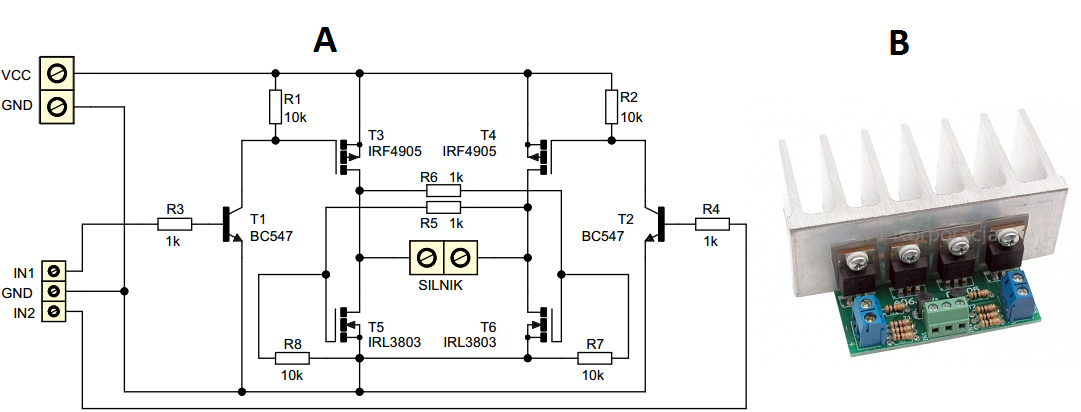
\includegraphics[scale=0.45]{imgs/mostek_h_schemat.png}
 	\caption[Schemat mostka H.]{\small{Ilustracja A przedstawia schemat ideowy mostka H, B - zdjęcie wykonanego mostka.}\footnotemark}
	\label{mostek_h_sch}
    \end{center}
  \end{figure}  
  	  \footnotetext{\emph{Mostek H}, http://sklep.avt.pl/,  (data dostępu 29.12.2015 r.)}
  	  
Część logiczna zasilana jest z 5 V źródła napięcia. Na oficjalnej stronie \textit{Raspberry Pi} napisane jest, że powinno się zastosować zasilacz o mocy około 10 W. Na pokładzie robota znajduje się 12 V bateria. Wystarczy zatem wykorzystać przetwornicę obniżającą napięcie - \textit{step-down}, która przedstawiona została na rysunku \ref{p_dc_dc_sch}. Ilustracja \ref{p_dc_dc_sch}A przedstawia schemat ideowy przetwornicy, której działanie opiera się o kluczowanie stałego napięcia wejściowego U$_1$ przy pomocy tranzystora K. Cewka L oraz kondensator C$_0$ magazynują energię dostarczoną podczas zwarcia klucza K, którą oddają w fazie rozwarcia. Zadaniem diody D jest zapewnienie odpowiedniego kierunku przepływu prądu. Napięcie wyjściowe U$_0$ odłożone na obciążeniu R$_0$ jest zależne od współczynnika wypełnienia kluczowanego napięcia. Na rysunku \ref{p_dc_dc_sch}B przedstawiona została wykorzystana przetwornica. 
\begin{figure}[H]
    \begin{center}
      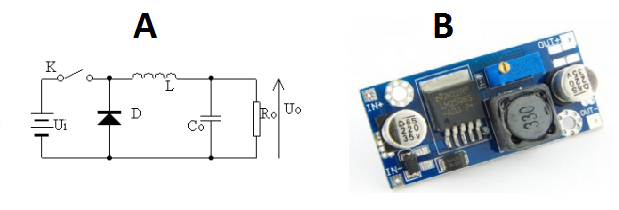
\includegraphics[scale=0.82]{imgs/przetwornica.png}
 	\caption[Przetwornica obniżająca napięcie DC/DC]{\small{Ilustracja A przedstawia schemat ideowy przetwornicy typu \textit{step-down}}\footnotemark \small{, B - zdjęcie wykorzystanej przetwornicy.}\footnotemark}
	\label{p_dc_dc_sch}
    \end{center}
  \end{figure}  
  	\footnotetext[2]{\emph{PRZETWORNICE IMPULSOWE – DŁAWIKOWE }, http://http://ue.pwr.wroc.pl/,  (data dostępu 29.12.2015 r.)}
  	  \footnotetext{\emph{Przetwornica napięcia DC-DC LM2596S}, http://http://electropark.pl/,  (data dostępu 29.12.2015 r.)}

Płytka realizująca funkcję sterownika silników napędowych została zaprojektowana od podstaw, w związku z tym posiada własny układ zasilający oparty o stabilizator liniowy 7805, którego schemat przedstawiony został na rysunku \ref{zas_at}. Zastosowany układ scalony odpowiedzialny jest przede wszystkim za obniżenie napięcia wejściowego do żądanej wartości. Dodatkowo posiada on także zintegrowane systemy chroniące go przed zwarciem oraz przegrzaniem. Układy logiczne wymagają dużej stabilności napięcia zasilającego, stąd też zarówno na wejściu jak i wyjściu układu zastosowane zostały dodatkowe kondensatory. Elementy C1, C4 to kondensatory elektrolityczne charakteryzujące się dużą pojemnością mogące skompensować stosunkowe duże wahania napięcia. C2 oraz C3 to kondensatory ceramiczne, które dobrze radzą sobie z szybkozmiennymi, niewielkimi zmianami.

  \begin{figure}[H]
    \begin{center}
      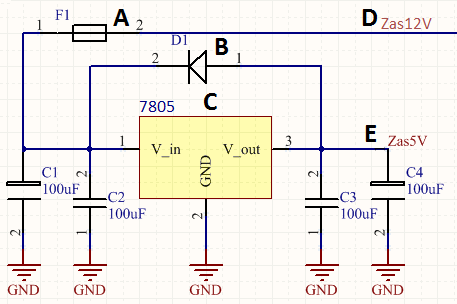
\includegraphics[scale=0.8]{imgs/zasilanie_atmeg.png}
 	\caption[Zasilanie sterownika silników.]{\small{Schemat ideowy układu zasilania, na którym: A - bezpiecznik nadmiarowo-prądowy (350mA), B - dioda mająca na celu zabezpieczenie układu przez przepięciami mogącymi pojawić się po stronie wyjściowej, C - liniowy stabilizator napięcia 7805, D - 12 V napięcie wejściowe, E - 5 V napięcie wyjściowe. Kondensatory C1, C2, C3 oraz C4 dodatkowo stabilizują napięcie.}}
	\label{zas_at}
    \end{center}
  \end{figure}  
  
Uruchomienie robota zrealizowane zostało przy wykorzystaniu pojedynczego włącznika, podłączonego szeregowo pomiędzy baterią a resztą pojazdu. Części wykonawcze robota (głównie silniki) potrafią pobierać bardzo duży prąd, w związku z tym przy wyborze elementu należy kierować się jego wytrzymałością prądową. Robot, w najgorszym przypadku, może pobierać około 13 A (silniki napędowe 2$\cdot$5 A, logika 3 A) co jest dość dużą wartością. Przełączniki mogące pracować w takich warunkach są duże i nieporęczne. Zastosowany został zatem przekaźnik wraz z układem pozwalającym na ograniczenie prądu płynącego przez jego cewkę (rys. \ref{wyla}). Czołg uruchamiany jest ręcznie przy wykorzystaniu przełącznika suwakowego A. Jego załączenie powoduje przepływ prądu przez cewkę przekaźnika B. Nominalny prąd płynący cewki w zastosowanym przekaźniku wynosi 30 mA, jednakże ,,pełną moc" cewki wykorzystuje się tylko w momencie załączenia styku - czyli bezpośrednio po włączeniu zasilania. Podtrzymywanie go w tej pozycji nie wymaga już tak dużego pola magnetycznego. Zastosowanie układu złożonego z rezystancji R oraz pojemności C pozwala na zmniejszenie prądu prądu płynącego przez układ. W chwili załączenia, gdy kondensator jest nienaładowany, traktowany jest jako zwarcie - przez układ płynie pełny prąd. Po chwili, gdy pojemność C się naładuje, jest ona rozwarciem, więc prąd będzie płynąć przez rezystancję R - będzie miał mniejszą wartość. Zastosowanie obciążenia o wartości odpowiadającej rezystancji cewki, czyli 400$\Omega$, zmniejsza jego wartość o połowę.

  \begin{figure}[H]
    \begin{center}
      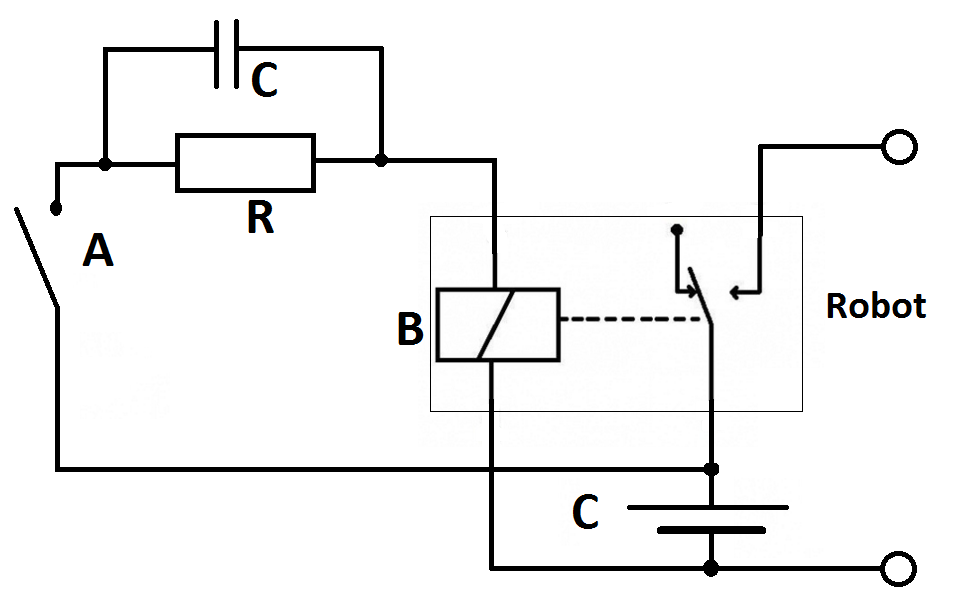
\includegraphics[scale=0.35]{imgs/wylaczniik.png}
 	\caption[Wyłącznik główny.]{\small{Schemat ideowy włącznika głównego zrealizowanego przy wykorzystaniu przekaźnika - B. Pozostałe elementy to: A - niewielki przełącznik suwakowy, C - bateria, R - rezystor, C - kondensator.}}
	\label{wyla}
    \end{center}
  \end{figure}   
  
  \namedsection{Podłączenie silników napędowych}
  Silniki sterowane są przez mostek H, który jest zbudowany w oparciu o tranzystory polowe. Elementy te są jednak stosunkowo wrażliwe na różnego rodzaju przepięcia oraz ładunki elektrostatyczne. Szczotkowe silniki prądu stałego w ogólności mogą być wykorzystane jako prądnice, co można zaobserwować mierząc napięcie na zaciskach obracającego się silnika. Zjawisko to może powstać w momencie odcięcia sygnału sterującego mostkiem H. Bezwładność pojazdu jeszcze przez chwilę będzie powodować obracanie się kół i generowanie ładunku. Aby zniwelować wpływ tego zjawiska na tranzystory zastosowano układ pokazany na rysunku \ref{diody}. Do tego celu wykorzystane zostały diody Schottky'ego, charakteryzujące się przede wszystkim niższym napięciem polaryzacji złącza p-n wynoszącym około 0,4~V.

  \begin{figure}[H]
    \begin{center}
      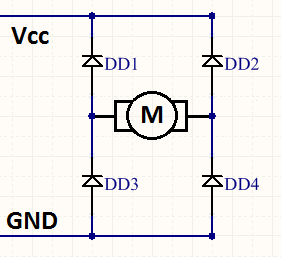
\includegraphics[scale=0.7]{imgs/silnik_pol.png}
 	\caption[Podłączenie silników napędowych.]{\small{Schemat ideowy układu odprowadzającego nadmiarowy ładunek z obwodu silników napędowych. Przedstawione elementy: DD1, DD2, DD3 oraz DD4 - diody Schottky'ego, Vcc - napięcie z baterii, GND - masa układu.}}
	\label{diody}
    \end{center}
  \end{figure}   
  
  \namedsection{Eliminacja drgań styków}
  Na płytce drukowanej znajdują się mikro przyciski oraz krańcówki, które są urządzeniami mechanicznymi - mogą wywoływać drgania podczas zwierania bądź rozwierania styków. Powstałe w ten sposób zakłócenie może niekiedy negatywnie wpływać na działanie zarówno układu jak i programu wyzwalając pewną funkcję niezliczoną liczbę razy. Aby przeciwdziałać temu zjawisku zastosowany został sprzętowy układ eliminujący drgania, który został przedstawiony na schemacie \ref{drg}. Zaprezentowane rozwiązanie utrzymuje wysoki stan logiczny dla rozwartego, nie wciśniętego przycisku. Najważniejszym elementem układu jest kondensator, który jako element całkujący usuwa składowe wysokoczęstotliwościowe - drgania. 
  
 \begin{figure}[H]
    \begin{center}
      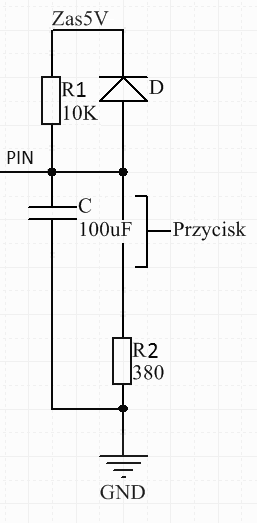
\includegraphics[scale=0.45]{imgs/drgania.png}
 	\caption[Eliminacja drgań styków.]{\small{Schemat ideowy układu eliminacji drgań styków. Rezystor R1 jest rezystorem podciągającym o wartości 10 k$\Omega$, D - dioda chroniąca układa przed przepieciami, C - kondensator, który tłumi drgania o pojemności 100 $\mu$F, R2 - rezystor ograniczający prąd zwarciowy płynący z kondensatora C po naciśnięciu przycisku o wartości 380 $\Omega$. PIN to wyprowadzenie prowadzące do wejścia mikrokontrolera. }}
	\label{drg}
    \end{center}
  \end{figure}   
  
  \namedsection{Realizacja magistrali TWI} 
  Magistrala TWI w ogólności wymaga jedynie podłączenia rezystorów podciągających dla linii komunikacyjnych co zostało przedstawione na schemacie \ref{podlaczenie_TWI}. W projekcie zastosowano do tego rezystory o wartości 4,7 k$\Omega$. Problem pojawił się jednak w przypadku wspólnego połączenia zastosowanych Atmeg48 oraz \textit{Raspberry Pi}. Mikrokontrolery pracują na napięciu 5 V - tak samo jak magistrala TWI. Druga platforma natomiast pracuje na napięciu 3,3 V. W związku z tym należało zastosować układ konwersji stanów logicznych, którego schemat został przedstawiony na schemacie \ref{konw_sch}. Jeżeli, tak jak w tym przypadku, Atmegi są zasilane ze źródła 5 V to jest to jedyne rozwiązanie. Minimalne napięcie umożliwiające prawidłową pracę, zgodnie z dokumentacją techniczną, wynosi $0,7\cdot 5V = 3,5 V$. Dla tego typu układów należy zastosować tranzystory (TR1 oraz TR2) dedykowane do konwersji stanów logicznych transmisji danych, czyli przystosowane do pracy przy wysokich częstotliwościach. Elementy tego typu charakteryzują się szczególnie małymi wartościami pojemności pasożytniczych.
  
\begin{figure}[H]
    \begin{center}
      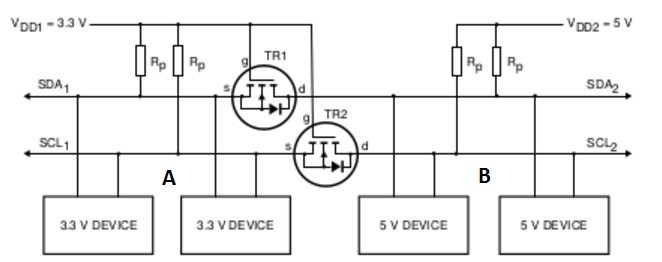
\includegraphics[scale=0.40]{imgs/konwersja.jpg}
 	\caption[Konwersja stanów logicznych.]{\small{Na rysunku przedstawiono schemat ideowy układu konwersji stanów logicznych opartego o dwa tranzystory polowe TR1 oraz TR2. Sekcja A to urządzenia pracujące z napięciem 3,3 V. Sekcja B - 5 V. Rezystory R$_p$ pełnią funkcję rezystorów podciągających.}\footnotemark}
	\label{konw_sch}
    \end{center}
  \end{figure}  
  	  \footnotetext{\emph{Raspberry Pi and I2C devices of different voltage}, http://nathan.chantrell.net/,  (data dostępu 30.12.2015 r.)}
  	  
  \namedsection{Rezonator kwarcowy}
  Rezonatory kwarcowe są układami służącymi do stabilizacji częstotliwości. Wykonane jako osobne komponenty (aby zapobiegać zakłóceniom) charakteryzują się wysoką jakością generowanego przebiegu. Ich głównym elementem jest kryształ kwarcu, który w wyniku pobudzenia polem elektrycznym zaczyna wibrować. Każdy rezonator ma ściśle określoną częstotliwość pracy, dla której występuje zjawisko rezonansu mechanicznego.  Atmega48 posiada wewnętrzny oscylator, jednakże umożliwia ona taktowanie jedynie z prędkością 8 MHz. Aby wykorzystać pełną moc układu należy zastosować rezonator kwarcowy o częstotliwości 20 MHz. Schemat przedstawiający sposób podłączenia elementu przedstawiona na rysunku \ref{xxtal}. Kondensatory C5 oraz C6 dodatkowo stabilizują ,,punkt pracy" układu. 
  
   \begin{figure}[H]
    \begin{center}
      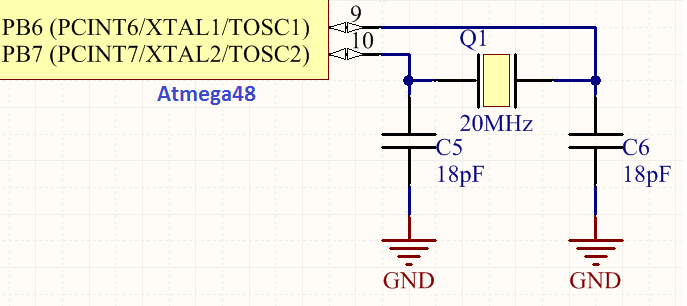
\includegraphics[scale=0.45]{imgs/xtal.png}
 	\caption[Podłączenie rezonatora kwarcowego.]{\small{Schemat ideowy przedstawia sposób podłączenia zewnętrznego oscylatora Q1 do mikrokontrolera. Wartość kondensatorów C5 oraz C6 określa dokumentacja techniczna układu. Ich zadaniem jest stabilizacja rezonansu kryształu kwarcowego. }}
	\label{xxtal}
    \end{center}
  \end{figure}   
  
\namedchapter[Adam Zieliński]{Projekt oraz wykonanie płytki drukowanej}
Płytka drukowana jest to płytka wykonana z tworzywa izolacyjnego, na którą naniesione zostały komponenty elektroniczne połączone miedzianymi ścieżkami. W ogólności jest to sposób montażu układów elektronicznych zapewniający estetyczną oraz kompaktową strukturę. Znajdujące się na niej obwody są projektowane ściśle pod konstruowany układ.
\namedsection{Projekt}
Pierwszym etapem projektowania jest zaplanowanie rozmieszczenia komponentów na jej powierzchni. Dzięki temu można określić ostateczne wymiary przygotowywanej powierzchni, które w tym przypadku wynoszą 85x155 mm. Specjalnie stworzone do tego środowisko pozwala płynnie przejść z schematu ideowego do ,,widoku" płytki uwzględniając przy tym wstępne połączenia pomiędzy elementami. Bardzo dużo uwagi należy poświęcić sprawdzeniu oznaczeń obudów zastosowanych układów oraz ich rozmiary, gdyż może okazać się, że zakupiony układ ma inny, niżeli wcześniej założony, kształt. W momencie, gdy wszystkie części są poukładane możemy rozpocząć proces łączenia sugerowanych przez środowisko pinów. Poprowadzone ścieżki powinny mieć określoną grubość - w zależności od wartości płynących przez nią prądów. Docelowo linie zasilające powinny być najszersze - tutaj 2 mm. Mimo licznych prób nie udało się poprowadzić wszystkich ścieżek na jednej stronie laminatu. W związku z tym zaprojektowana została płytka dwustronna - czyli posiadająca ścieżki po obu stronach. Ścieżki połączone zostały przez tzw. przelotki, czyli niewielkie miedziane druty przechodzące przez laminat. Wszystkie wykorzystane elementy pozwalają na montaż przewlekany, przez co niezbędne jest wykonanie w płytce otworów przeznaczonych na wyprowadzenia elementów. Wyprowadzenia te zrealizowane są w formie drucików, które przewleka się przez otwory i lutuje do ścieżki. Rysunek \ref{plyta} przedstawia ostateczny projekt płytki drukowanej. Część A to warstwa dolna, do której przylutowane zostały komponenty, B - wierzchnia.

   \begin{figure}[H]
    \begin{center}
      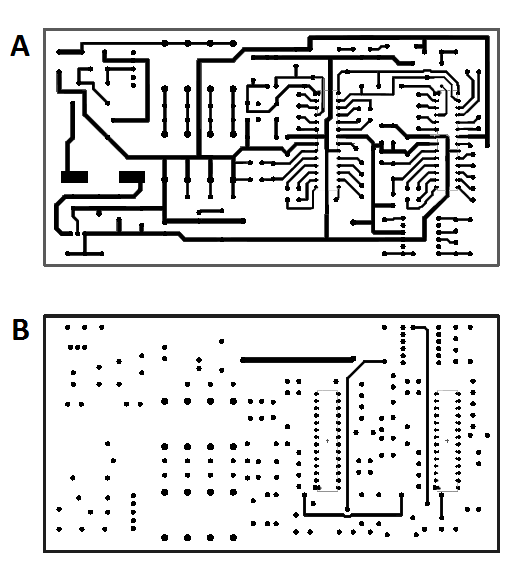
\includegraphics[scale=0.7]{imgs/plytka.png}
 	\caption[Projekt płytki drukowanej.]{\small{Rysunek przedstawia finalny projekt płytki drukowanej. Segment A przedstawia dolną jej dolną część - do której elementy są przylutowane, B - wierzchnią. }}
	\label{plyta}
    \end{center}
  \end{figure}   
\namedsection{Wykonanie}
Wykonanie płytki drukowanej należy rozpocząć od przeniesienie gotowego projektu bezpośrednio na powierzchnię pokrytą miedzią. Do tego celu wykorzystany został papier kredowy oraz drukarka laserowa. Wspomniany papier jest bardzo śliski oraz bardzo słabo ,,łączy" się z tonerem. Dzięki temu wydrukowany na niej układ stosunkowo słabo przywiera do jej powierzchni - co umożliwia jego dalszy transfer. Odpowiednio skrojony fragment laminatu należy bardzo bardzo dokładnie odtłuścić, np. przy użyciu acetonu. Opcjonalnie można także jego powierzchnię nieco zmatować przy wykorzystaniu papieru ściernego o wysokiej granulacji. Kolejnym etapem jest odbicie projektu na laminacie. W związku z tym papier kredowy należy możliwie dokładnie umieścić na płytce drukiem do jej powierzchni oraz zgrzać np. żelazkiem. Toner w temperaturze około 200$^\circ$C topi się i ,,odrywa" od papieru przywierając do miedzianej warstwy. Następnie wystarczy delikatnie usunąć papier. Nadrukowane tonerem ścieżki pozostają na płytce. Pozostaje jedynie umieścić płytkę w wytrawiaczu - nadsiarczanie sodu. Jest to środek o silnych właściwościach utleniających. Jego wodny roztwór wchodzi z reakcję z niezakrytą tonerem miedzią, utlenia ją i rozpuszcza.  Poniżej (rys. \ref{trwa}) znajdują się zdjęcia przedstawiające laminat bezpośrednio przed (A) oraz po (B) trawieniu. Kąpiel w utleniaczu powinna trwać tak długo, do momentu aż miedź całkowicie nie zniknie.

   \begin{figure}[H]
    \begin{center}
      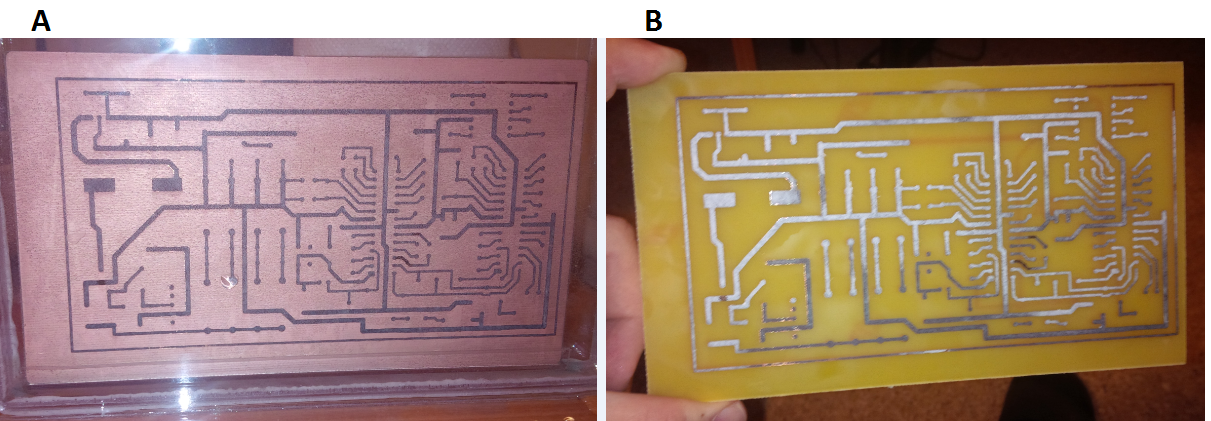
\includegraphics[scale=0.47]{imgs/plytka_trawienie.png}
 	\caption[Proces trawienia.]{\small{Zdjęcia przedstawiają pierwszy etap wykonywania płytki drukowanej. Fotografia A przedstawia laminat z przeniesionymi ścieżkami, umieszczony w wytrawiaczu. B - efekt wytrawienia.}}
	\label{trwa}
    \end{center}
  \end{figure}  
  
  Ostatnim etapem jest przylutowanie wszystkich komponentów. Efekt końcowy został przedstawiony na zdjęciach \ref{ost_ef}.
  
  \begin{figure}[H]
    \begin{center}
      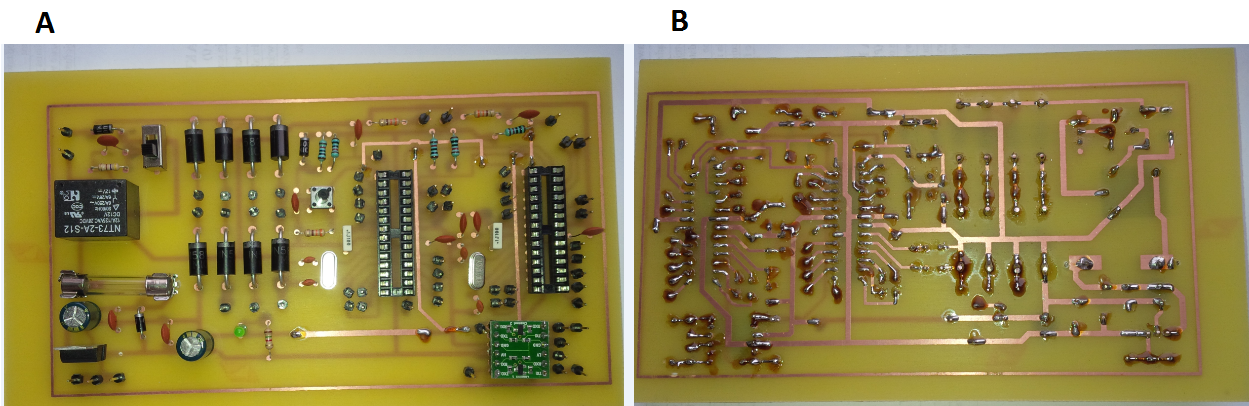
\includegraphics[scale=0.45]{imgs/efekt.png}
 	\caption[Wykonanie płytki drukowanej.]{\small{Zdjęcia przedstawiają kompletną, działająca płytkę drukowaną. Fotografia A przedstawia warstwę górną, B - warstwę dolną.}}
	\label{ost_ef}
    \end{center}
  \end{figure}  
\namedchapter[Adam Zieliński]{Sterownik silników}
Sterownik silników został zaimplementowany na dwóch mikrokontrolerach z rodziny AVR. Każdy z nich sterowany jest przy wykorzystaniu osobnego układu. Realizacja regulatora wymaga obsługi pętli sprzężenia zwrotnego od prędkości obrotowej, zgodnie z schematem przedstawionym na rysunku \ref{schem_ster}. 

  \begin{figure}[H]
    \begin{center}
      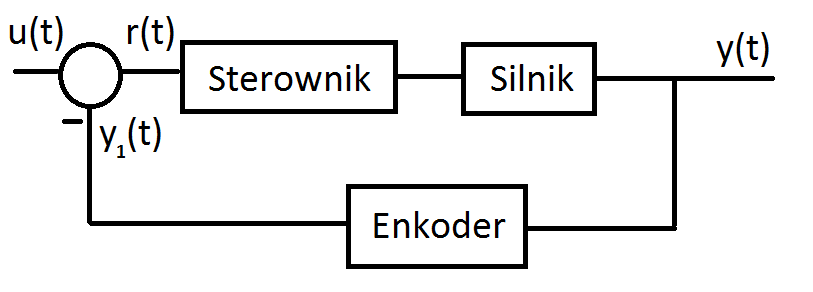
\includegraphics[scale=0.45]{imgs/sterowanie.png}
 	\caption[Schemat pętli sterowania silnikami.]{\small{Schemat przedstawia koncepcję pętli sterowania silnikami napędowymi. Ujemne sprzężenie zwrotne realizowane jest przy wykorzystaniu enkodera impulsowego. Sygnały: $u(t)$ - wartość zadana, $r(t)$ - uchyb, $y(t)$ wyjście układu, $y_1(t)$ - sygnał wyjściowy enkodera.}}
	\label{schem_ster}
    \end{center}
  \end{figure}  
  
\namedsection{Programowanie}
Programowanie Atmegi odbywa się przy wykorzystaniu programatora, czyli specjalnego układu elektronicznego służącego do sprzęgnięcia komputera z mikrokontrolerem zgodnie z rysunkiem \ref{schem_ster}. Urządzenie realizuje komunikację jednostronną, tzn. przesyła jedynie program do wewnętrznej pamięci układu scalonego.  Programowanie odbywa się przy wykorzystaniu magistrali SPI, która ,,wybiera" układ docelowy przy pomocy linii SS (ang. \textit{Slave Select}) a następnie przesyła dane wykorzystując linie MISO, MOSI. Linia SCK służy do synchronizacji przebiegów szeregowych. Z racji tego, że programowany jest tylko jeden, aktualnie podłączony układ, linię SS można zaniechać.

  \begin{figure}[H]
    \begin{center}
      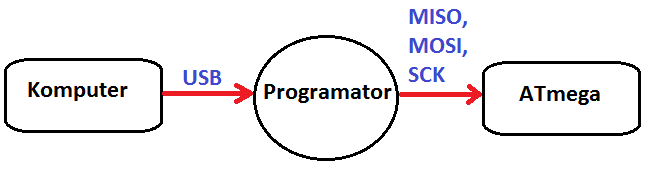
\includegraphics[scale=0.7]{imgs/schemat_prog.png}
 	\caption[Podłączenie programatora.]{\small{Graf przedstawiający idee pracy programatora. ATmega przyjmuje dane posługując się następującymi pinami : MISO (ang. \textit{Master Input Slave Output} - przyjmowanie danych), MOSI (ang. \textit{Master Output Slave Input} - nadawanie danych) oraz SCK - zegar taktujący. Wymienione piny pozwalają na realizacje transmisji typu SPI (ang. \textit{Serial Peripheral Interface}) pozwalającej na komunikacje jednostki centralnej z układami peryferyjnymi.}}
	\label{schem_ster}
    \end{center}
  \end{figure}  
  
\namedsection{Prędkość obrotowa}
Częstotliwość obrotu jest odczytywana przy wykorzystaniu enkoderów impulsowych. W jego skład wchodzi niewielkie koło, na którego obwodzie obsadzone są magnesy. Urządzenie pomiarowe jest układem scalonym umieszczonym nieco ponad obracającym się kołem. Czujnik działa w oparciu o efekt Halla i na wyjściu generuje falę prostokątną o liczebności około 355 impulsów na jeden pełny obrót koła. Częstotliwość obrotu kół jest obliczana na podstawie częstotliwości wspomnianej fali prostokątnej. Pomiar realizowany jest na przy wykorzystaniu wewnętrznego licznika - Timer1. Jest on taktowany wewnętrznym sygnałem zegarowym CLK. Każdy jego takt zwiększa wartość licznika TCNT1 (ang. \textit{Timer Counter 1}) o 1. Do pinu zewnętrznego pinu ICP1 (ang. \textit{Input Capture 1}) podłączony zostaje enkoder. Zbocze narastające sygnału z enkodera powoduje przepisanie aktualnej wartości z rejestru TCNT1 do rejestru ICR1 (ang. \textit{Input Capture Register 1}). W ten sposób ICR1 przechowuje ilość taktów wewnętrznego zegara przypadających pomiędzy dwoma narastającymi zboczami sygnału z enkodera. Wartość częstotliwości obrotu kół obliczona zostaje z zależności \ref{eq:czest_kola}. Aby zwiększyć dokładność pomiaru wszystkie wyniki zostały pomnożone razy 10.
\begin{equation}
	f_{kół} =  \frac{f_{cpu} \cdot 10}{p_r \cdot n_i \cdot L_{ICR1} } 
   \label{eq:czest_kola}
 \end{equation}
 gdzie:  
 \begin{equationDescriptor}
   \EQDitem{$f_{kół}$}{częstotliwość obrotu koła [Hz],}
 	\EQDitem{$f_{cpu}$}{częstotliwość taktowania mikrokontrolera [Hz],}
 	 \EQDitem{$p_r$}{wartość prekalera dla sygnału CLK,}
 	  \EQDitem{$n_i$}{ilość impulsów przypadająca na jeden pełny obrót koła, }
 	   \EQDitem{$L_{ICR1}$}{wartość zapisana w rejestrze ICR1.}
 \end{equationDescriptor} 

  \begin{figure}[H]
    \begin{center}
      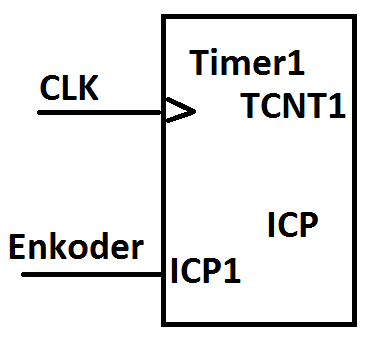
\includegraphics[scale=0.4]{imgs/predkosc.png}
 	\caption[Pomiar częstotliwości obrotu silnika.]{\small{Ilustracja przedstawia ideę pomiaru częstotliwości obrotu silników napędowych. Timer1 jest wewnętrznym, sprzętowym licznikiem mikrokontrolera. Na wyprowadzeniu pinu Atmegi ICP1 podłączony jest enkoder. Licznik taktowany jest wewnętrznym zegarem. W momencie wystąpienia zbocza narastającego na pinie ICP1 aktualna wartość licznika, przechowywana w rejestrze TCNT1 zapisywana jest do rejestru ICR1. Znając szybkość taktowania licznika oraz ilość zliczonych impulsów pomiędzy dwoma narastającymi zboczami enkodera możliwe jest obliczenie częstotliwości obrotu wału silnika.}}
	\label{predkosc}
    \end{center}
  \end{figure}  
  Poniższy kod inicjalizuje opisany wcześniej licznik. Makrodefinicja \_BV() zwraca 8-bitową liczbę z wartością 1 na wskazanej w nawiasie pozycji, np. \_BV(3) = 0000 0100. Pin ICP1 jest 14 pinem mikrokontrolera, najmniej znaczącym bitem rejestru wyjściowego PB. Z racji tego, że może pełnić kilka funkcji należy go odpowiednio zdefiniować. Ustawiany jest jako wejście (poprzez wpisanie do rejestru DDRB (ang. \textit{Data Direction Register B}) wartości 1 na jego pozycji PB0) oraz wewnętrznie ściągany do stanu logicznego 0 (poprzez przypisanie wartości 0 w rejestrze PORTB). Znak '\textasciitilde' tworzy bitową negację zapisanej za nią liczby. Operator '\&=' realizuje operację iloczynu bitowego. Kolejnym etapem jest konfiguracja licznika. Służy do tego rejestr TCCR1 (ang. \textit{Timer Counter Control Register 1}) dzielący się na dwie 8-bitowe sekcje: A i B. Ustawienie flagi ICNC1 (ang. \textit{Input Capture Noise Canceler}) rozpoczyna realizację usuwania szumów z odbieranego sygnału. Proces polega na zapamiętywaniu czterech kolejnych próbek sygnału podawanego na pin ICP1. Aktualizacja odczytanego poziomu sygnału przez mikrokontroler odbędzie się dopiero po odebraniu czterech, jednakowych próbek. Ustawienie bitu ICES1 (ang. \textit{Input Capture Edge Select}) nastawia wyzwalanie przechwycenia przy wystąpieniu zbocza narastającego. Timer1 jest licznikiem 16-bitowym. Aby móc prawidłowo odczytać częstotliwość nie można dopuścić aby pomiędzy kolejnymi zboczami sygnału enkodera doszło do przepełnienia licznika (sytuacja ta odpowiada najmniejszej możliwej do odczytania przez układ częstotliwości $f=\frac{f_{cpu}}{2^{16}}$).
Dolna granica pomiaru może zostać przesunięta przy wykorzystaniu preskalera, czyli układu realizującego podział częstotliwości. Jego wartość ustawia się w rejestrze TCCR1B poprzez odpowiednią, znajdującą się w nocie katalogowej układu \cite{nota}, konfigurację bitów CS (ang. \textit{Clock Select}). Odbierane z enkodera sygnały mogą pojawić się w dowolnej chwili z dowolną częstotliwością. W związku z tym niezbędne obliczenia wykonywane będą w przerwaniach. Uruchomienie ich obsługi odbywa się poprzez ustawienie bitu ICIE (ang. \textit{Input Capture Interrupt Enable}) odpowiedzialnego za uruchomienie przerwania związanego z wystąpieniem zdarzenia związanego z wejściem przechwytującym oraz TOIE (ang. \textit{Timer Overflow Interrupt Enable}) związanego z przepełnieniem licznika.
  \begin{lstlisting}
DDRB &= ~(_BV(PB0));                 ustawienie pinu ICP1 jako wejscie 
PORTB &= ~(_BV(PB0))                 pin przyjmuje wartosc logiczna 0
TCCR1B = _BV(ICNC1) | _BV(ICES1);    ICNC1 - ustawienie filtrowania wejscia ICNC1
                                     ICES1 - wyzwalanie zboczem narastajacym 
TCCR1B |= _BV(CS21) | _BV(CS20);     ustawienie wartosci preskalera na 64
TIMSK1 = _BV(ICIE1) | _BV(TOIE1);    uruchomienie obslugi przerwan
\end{lstlisting}

\namedsection{Generacja sygnału PWM}
Silniki sterowane są przy wykorzystaniu sygnału PWM. Generowany jest on sprzętowo, wykorzystując wewnętrzny licznik mikrokontrolera. Czynny udział w tym procesie bierze udział rejestr TCNT0 oraz OCRA0 (ang. \textit{Output Compare Register}, sekcja A). Tak jak w przypadku pomiaru częstotliwości, rejestr TCNT0 przechowuje aktualny stan licznika. Do OCRA0 wpisujemy dowolną, 8-bitową liczbę. W momencie gdy wartość TCNT0 oraz OCRA0 są sobie równe, stan na wyjściu mikrokontrolera (na pinie OC0A) ulega zmienia. W przypadku wpisania do rejestru porównującego wartości 128, otrzymujemy na wyjściu sygnał o wypełnieniu 50~\%. Działanie układu przedstawiono na rysunku \ref{gen_pwn}.
\newpage
\begin{figure}[H]
    \begin{center}
      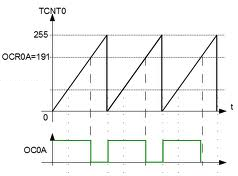
\includegraphics[scale=0.9]{imgs/pwm_gen.png}
 	\caption[Realizacja sygnału PWM.]{\small{Ilustracja przedstawia sposób generowania sygnału PWM przy wykorzystaniu 8-bitowego licznika. W rejestrze TCNT0 znajduje się aktualna wartość licznika, która jest inkrementowana wraz z każdym taktem zegara. Zmienia się od 0 do 255. Do rejestru OCRA0 wpisana jest wartość 191. Jest to wartość porównawcza. W momencie zrównania się wartości OCRA0 oraz TCNT0 sygnał na wyjściu, na pinie OC0A ulega zmianie.}\footnotemark}
	\label{gen_pwn}
    \end{center}
  \end{figure}  
  	  \footnotetext{\emph{Aplikasi PWM Mikrokontroler ATmega8535}, http://ediamon.files.wordpress.com/,  (data dostępu 03.01.2016 r.)}
\noindent
Poniżej przedstawiono proces inicjalizacji trybu PWM licznika. Kod sprowadza się do odpowiedniego ustawienia bitów rejestrów kontrolnych TCCR. Flagi WGM (ang. \textit{Waveform Generation Mode}) służą do wyboru trybu pracy licznika - zgodnie z dokumentacją techniczną mikrokontrolera\cite{nota}. 
  \begin{lstlisting}
TCCR2A |= _BV(WGM20) | _BV(WGM21);   // tryb PWM
TCCR2B =  _BV(CS21) | _BV(CS20);     // preskaler 32
\end{lstlisting}
\noindent
Dodatkowo należy także wybrać częstotliwość generowanego przebiegu, która w tym przypadku wynosi:
\begin{equation}
	f_{PWM} =  \frac{f_{cpu}}{N \cdot 256} = \frac{20 \cdot 10^6}{256 \cdot 32} = 4882 
   \label{eq:czest_kola}
 \end{equation}
 gdzie:  
 \begin{equationDescriptor}
   \EQDitem{$f_{PWM}$}{częstotliwość sygnału PWM [Hz],}
 	\EQDitem{$f_{cpu}$}{częstotliwość taktowania mikrokontrolera [Hz],}
 	 \EQDitem{$N$}{wartość prekalera licznika.}
 \end{equationDescriptor}
\noindent
Dla wyższych częstotliwości pozostawały one w stanie nasycenia - nie realizowały kluczowania. 

Funkcja sterująca generowanym sygnałem pobiera dwa argumenty odpowiedzialne kolejno za obrót w przód oraz w tył. Przez wzgląd na konstrukcję mostka H należało wykonać sterowanie przy wykorzystaniu dwóch osobnych sygnałów PWM. Konstrukcja Atmegi pozwala na wytworzenie dwóch przebiegów przy wykorzystaniu jednego licznika, o tej samej częstotliwości ale innym wypełnieniu. Argumenty pwm\_1 oraz pwm\_2 to wartości porównujące licznika i są przypisywane do rejestrów OCR. Sterują one wypełnieniem sygnału uzyskanego na pinach OC2A (ang. \textit{Output Compare}) i OC2B. Wytworzenie przebiegu jednocześnie na obu pinach zakończyłoby się zwarciem oraz zniszczeniem mostka H. Warunkowa struktura funkcji zabezpiecza układ przed tą możliwością. Dopuszcza generację tylko jednego, określonego sygnału. 
\begin{lstlisting}
void ster_silnik(unsigned char pwm_1, unsigned char pwm_2)
{
	if (pwm_1 == 0x00 && pwm_2 != 0x00 ) //obrot w tyl
	{
		TCCR2A &= ~(_BV(COM2A1)); // zaprzestanie generacji sygnalu
		DDRB &= ~(_BV(PB3)); 	  // ustawienie pinu OCR2A jako wejscie
		PORTB &= ~(_BV(PB3));     // przypisanie wartosci 0
		//ustawienie OCR2B
		TCCR2A |= _BV(COM2B1);    // uruchomienie pinu wyjsciowego
		DDRD |= _BV(PD3);         // ustawienie go jako wyscie
		OCR2B = pwm_2;            // przypisanie wartosci porownujacej
	}
	else if (pwm_2 == 0x00 && pwm_1 != 0x00 ) // obrot w przod
	{
		TCCR2A &= ~(_BV(COM2B1)); // zaprzestanie generacji sygnalu
		DDRD &= ~(_BV(PD3));      // ustawienie pinu OCR2A jako wejscie
		PORTD &= ~(_BV(PD3));     // sciagniecie do GND
		//ustawienie OCR2A
		TCCR2A |= _BV(COM2A1);    // uruchomienie pinu wyjsciowego
		DDRB |= _BV(PB3);         // ustawienie go jako wyjscie
		OCR2A = pwm_1;            // przypisanie wartosci porownujacej
	}
	else // rozlaczenie pinow
	{
		TCCR2A &= ~(_BV(COM2A1) | _BV(COM2A0)); 
		DDRB &= ~(_BV(PB3)); 
		PORTB &= ~(_BV(PB3)); 
		TCCR2A &= ~(_BV(COM2B1) | _BV(COM2B0)); 
		DDRD &= ~(_BV(PD3)); 
		PORTD &= ~(_BV(PD3)); 
	}
}
\end{lstlisting}

\namedsection{Implementacja TWI}
Zastosowane mikrokontrolery posiadają sprzętowe wsparcie dla realizacji komunikacji TWI. Dzięki niej nie ma potrzeby implementowania całej komunikacji od podstaw. Wystarczy jedynie odpowiednia konfiguracja poszczególnych bitów znajdujących się w rejestrze konfiguracyjnym TWCR (ang. \textit{TWI Control Register})\cite{nota}. Flaga: TWEN (ang. \textit{TWI Enable}) ,,uruchamia" TWI, TWIE (ang. \textit{TWI Interrupt Enable}) włącza obsługę przerwania związanego z tym interfejsem, TWEA (ang. \textit{TWI Enable Acknowlage}) steruje generowaniem bitu potwierdzającego. Kolejnym etapem jest przygotowanie 7 bitowego adresu urządzenia. Znajduje się on w rejestrze TWAR (ang. \textit{TWI Address Register}), zapisany na bitach 7..1. W związku z tym jego wartość, zapisaną w zmiennej ad\_s, należy przesunąć o jedną pozycję w lewo. 
\begin{lstlisting}
TWCR = _BV(TWEN) | _BV(TWIE) | _BV(TWEA);
ad_s = ad_s<<1;  //przesuniecie adresu o jedna pozycje bitowa w lewo
TWAR = ad_s;     //wpisanie przygotowanego adresu
\end{lstlisting}
Układ pracuje w trybie \textit{Slave}, co oznacza, że nie będzie nigdy pierwszy rozpoczynał transmisji a jedynie odpowiadał na zapytania od \textit{Mastera}. Odbiór przez urządzenie swojego adresu powoduje wyzwolenie przerwania związanego z transmisją TWI. Zmienna TWI\_TWSR zawiera w sobie definicje kodów związanych z poszczególnymi etapami komunikacji. Kody są ściśle określone przez producenta oraz zawarte w nocie katalogowej\cite{nota}. Rejestr TWDR (ang. \textit{TWI Shift Data Register}) przechowuje,odbiera oraz wysyła dane na magistralę. Poniższy kod służy implementacji trybu nadawczego układu podrzędnego. Kod 0xA8 informuje o tym, że urządzenie nadrzędne chce odczytać z ,,nas" daną (wybrany\_pomiar), którą należy umieścić w rejestrze TWDR. Gotowość urządzenia do transmisji sygnalizujemy ustawieniem flag TWINT, TWEA, TWIE oraz TWEN. Kod 0xB8 służy do wygenerowania bitu potwierdzającego. Natomiast 0xC0 odpowiada za zakończenie transmisji.
\begin{lstlisting}
switch(TWI_TWSR)
{
	//slave transmiter
	case TWI_STX_ADR_ACK: //0xA8
		TWDR = wybrany_pomiar(TWI_Buf[0]);
		TWCR = _BV(TWINT) | _BV(TWEA) | _BV(TWIE) | _BV(TWEN);
		break;
	case TWI_STX_DATA_ACK: //0xB8
		TWCR = _BV(TWINT) | _BV(TWIE) | _BV(TWEN);
		break;
	case TWI_STX_DATA_NACK: //0xC0
		TWCR = _BV(TWINT) | _BV(TWEA) | _BV(TWIE) | _BV(TWEN);
		break;
}
\end{lstlisting}
Poniżej znajduje się ciąg dalszy kodu, który jest odpowiedzialny za odbiór informacji. Kod dostosowany jest do przyjmowania dwóch bajtów danych zapisywanych w tablicy TWI\_Buf. Kod 0x60 sygnalizuje poprawną identyfikację adresu podanego na magistrali. Następnie poprzez ustawienie bitów rejestru TWCR układ sygnalizuje gotowość do odbioru. Odbiór danych realizowany się po wystąpieniu kodu 0x80. Zmienna TWI\_INT\_licznik odlicza ilość odebranych danych. Jest ona zerowana przed rozpoczęciem transmisji. Łączność kończy odebranie przez układ sygnału stopu (kod 0xA0). W nim odebrane dane są przypisywane do zmiennych zad\_f\_1 oraz zad\_f\_2, które następnie są przetwarzane w pętli głównej programu.
\begin{lstlisting}
case TWI_SRX_ADR_ACK: //0x60
	TWI_INT_licznik = 0;
	TWCR = _BV(TWINT) | _BV(TWEA) | _BV(TWIE) | _BV(TWEN);
	break;
	
case TWI_SRX_STOP_RESTART: //0xA0
	TWCR = _BV(TWINT) | _BV(TWIE) | _BV(TWEN) | _BV(TWEA);
	if(TWI_INT_licznik == TWI_wielkosc_ramki)
	{
		zad_f_1 = TWI_Buf[0];
		zad_f_2 = TWI_Buf[1];
	}
	break;

case TWI_SRX_ADR_DATA_ACK: // 0x80
	if(TWI_INT_licznik < TWI_wielkosc_ramki)
		TWI_Buf[TWI_INT_licznik++] = TWDR;
	TWCR = _BV(TWINT) | _BV(TWEA) | _BV(TWIE) | _BV(TWEN);
	break;
\end{lstlisting}

\namedsection{Implementacja regulatora P}
Sterowanie napędem odbywa się przy wykorzystaniu regulatora P, składającego się jedynie z członu proporcjonalnego. Transmitancja, czyli zależność pomiędzy wyjściem a wejściem układu, opisana jest wzorem:
\begin{equation}
	G_{p}(s) =  k_p 
   \label{eq:reg}
 \end{equation}
 gdzie:  
 \begin{equationDescriptor}
   \EQDitem{$G_{p}(s)$}{transmitancja,}
 	\EQDitem{$k_{p}$}{wzmocnienie członu proporcjonalnego.}
 \end{equationDescriptor}
 \noindent
 Na rysunku \ref{schem_ster_2} przedstawiony został schemat blokowy przedstawiający strukturę zaimplementowanego sterownika.
   \begin{figure}[H]
    \begin{center}
      \includegraphics[scale=0.45]{imgs/sterowanie2.png}
 	\caption[Schemat zrealizowanego sterownika.]{\small{Schemat przedstawia układ sterowania silnikami napędowymi. Ujemne sprzężenie zwrotne realizowane jest przy wykorzystaniu enkodera impulsowego, którego sygnał jest interpretowany przez mikrokontroler. Sygnały: $u(t)$ - wartość zadana, $r(t)$ - uchyb, $y(t)$ wyjście układu, $y_1(t)$ - sygnał wyjściowy enkodera.}}
	\label{schem_ster_2}
    \end{center}
  \end{figure}  
Układ charakteryzuje się niezerowym uchybem ustalonym, co w tym przypadku jest do zaakceptowania. Sygnał sterujący regulatora $r(t)$ możemy zapisać jako:
\begin{equation}
	r(t)=u(t)-y_1(t)
   \label{eq:reg1}
 \end{equation}
 gdzie:  
 \begin{equationDescriptor}
   \EQDitem{$r(t)$}{sygnał sterujący regulatorem,}
 	\EQDitem{$u_{t}$}{wartość zadana,}
 	 \EQDitem{$y_1(t)$}{sygnał otrzymany z sprzężenia zwrotnego.}
 \end{equationDescriptor}
 \noindent
 Wartość $r(t)$ nazywana jest uchybem, czyli różnicą pomiędzy wartością zadaną a rzeczywistą. Zadaniem regulatora P jest zapewnienie odpowiedniego wzmocnienia tego sygnału. Wartość wypełnienia sygnału PWM zawiera się w przedziale od 0 do 255. W związku z tym sygnał wyjściowy z regulatora należało odpowiednio ograniczyć. Fragment kodu zaprogramowanego na Atmegach został przedstawiony poniżej.
\begin{lstlisting}
char regulator(char we, char wy)  // we - zadana wartosc, wy - odczytana
{
	int k_p = 30;                 // deklaracja wzmocnienia czlonu P
	int uchyb = 0;                // deklaracja zmiennej uchybu
	int p = 0;                    // deklaracja zmiennej odpowiedzi regulatora
	unsigned char wyjscie = 0;    // deklaracja zmiennej wyjsciowej
	uchyb = (int)(we) - (int)(wy);// obliczanie uchybu
	p = k_p*uchyb;                // obliczanie odpowiedzi regulatora
	if (p > 255)                  // jezeli odpowiedz jest wieksza od 255
	    wyjscie = 0xFF;           // ustaw na wyjsciu wartosc 255
	else if(p < 0)                // jezeli odpowiedz jest mniejsza od 0
	    wyjscie = 0x00;           // ustaw na wyjsciu wartosc 0
	else                          // w przeciwnym wypadku
        wyjscie = (unsigned char)(p);
	return wyjscie;               // zwrocenie wartosci przez funkcje
}
\end{lstlisting}


\namedchapter[Daniel Łukwiński]{Algorytm rozpoznawania celu}
Wstęp.

\namedsection{Rodzaj celu}
Zadanie, jakie miał realizować robot polegało na namierzeniu oraz śledzeniu celu w swoim otoczeniu. Na początkowym etapie pracy należało ustalić, co ma być poszukiwanym przez czołg celem. Ostateczny wybór padł na czerwony okrąg, a więc obiekt o określonym kolorze oraz geometrycznym kształcie. Przy jego wyborze kierowano się tym, aby dany obiekt nie występował przypadkowo w otoczeniu, a jednocześnie nie odróżniał się od niego w nadzwyczajny sposób. Założeniem było także to, aby algorytm robota potrafił znajdować cel przy zróżnicowanym oświetleniu oraz na różnej odległości (tj. niezależnie od jego rozmiaru na obrazie). Ważne było także, aby celem mógł być każdy obiekt spełniający podstawowe warunki koloru i kształtu, a więc algorytm nie mógł być tworzony pod jeden konkretny obiekt służący za cel.

\namedsection{OpenCV}
OpenCV jest biblioteką służącą do wszechstronnej obróbki obrazu, wydaną na licencji BSD (\textit{Berkeley Software Distribution}), będącej zgodną z zasadami wolnego oprogramowania. Została ona napisana w C oraz C++, jednak możliwe jest je wykorzystywanie także w języku \textit{Python} oraz \textit{Java}. Wspiera ona takie systemy operacyjne jak: \textit{Windows, Linux, Mac OS, iOS} oraz \textit{Android}. Posiada ona moduły służące do pracy tak z obrazem dwuwymiarowym, jak i trójwymiarowym. Ponadto zawiera szereg modułów, służących między innymi do rozpoznawania twarzy, gestów czy systemów uczących się (ang. \textit{machine learning}).

O jej wykorzystaniu, poza darmową licencją, zdecydowała optymalizacja zastosowanych rozwiązań oraz mnogość funkcji, spełniających większość zadań związanych z analizą obrazu. Wykorzystywana w projekcie wersja nosi oznaczenie 3.0.0 i została opublikowana 4 czerwca 2015 roku. W przedstawianym algorytmie wykorzystywane są trzy moduły z tej biblioteki:
\begin{itemize}
\item \texttt{core.hpp} - zawiera podstawowe klasy oraz funkcje związane z pracą na obrazach dwuwymiarowych;
\item \texttt{imgproc.hpp} - zawiera bardziej zaawansowane funkcje służące to przetwarzania obrazów, np.: filtrację obrazu czy progowanie;
\item \texttt{highgui.hpp} - w tym pliku znajdują się funkcje związane z interface'm programu, które zostały wykorzystane jedynie na etapie tworzenia algorytmu, do testowania jego efektów efektów (wyświetlenie obrazu, odczyt oraz zapis do pliku).
\end{itemize}

\namedsection{Inicjalizacja}
Działający na Raspberry Pi program składa się z dwóch części. Pierwsza z nich jest odpowiedzialna za inicjalizację sprzętowych generatorów sygnału PWM na Raspberry oraz łączenie się z kamerą oraz rozpoczęcie jej pracy z ustalonymi parametrami.

Inicjalizacja sygnałów PWM na Raspberry jest wykonywana z wykorzystaniem biblioteki \textit{wiringPi}. Jest to napisana w języku C biblioteka obsługująca piny GPIO mini komputera Raspberry Pi. Została ona wydana na licencji \textit{GNU LGPLv3}, umożliwiającej darmowy dostęp dla wszystkich zainteresowanych użytkowników. Pierwszym krokiem inicjalizacji sygnałów PWM jest wywołanie funkcji \texttt{int wiringPiSetupGpio()}. Znajdują się w niej deklaracje niezbędne do poprawnej pracy z biblioteką. Odpowiada ona także za umożliwienie bezpośredniego dostępu do pinów GPIO Raspberry. Wartością zwracaną przez tą funkcję jest kod, informujący o poprawności wywołania. Jego wartość równa -1 oznacza błąd uniemożliwiający dalszą prawidłową pracę. Następnie należy wywołać funkcję \textit{void pinMode (int pin, int mode)}, której zadaniem jest ustawienie jednego z pinów GPIO Rasppbery w odpowiedni tryb: wejścia, wyjścia, wyjścia zegara lub wyjścia sygnału PWM. W tym przypadku koniecznie jest ustawienie pinów numer 18 oraz 19 jako wyjścia sygnału PWM. Kolejną wywoływaną funkcją z tej biblioteki jest void \texttt{pwmSetMode(int mode)}. Ma ona za zadanie ustalić w którym z dwóch trybów ma pracować generator sygnału PWM: \textit{mark:space} lub \textit{balanced}. Pierwszy z nich jest klasycznym sygnałem PWM, w którym okres sygnału jest równy całemu cyklowi pracy jego licznika. W drugim wartość wypełnienia jest równomiernie rozłożona na cykl liczniki, przez wyjściowa częstotliwość sygnału jest dużo większa. W zastosowanym algorytmie wykorzystany został pierwszy tryb, gdyż dużo lepiej nadaje się on do sterowania serwomechanizmów. Kolejne dwa niezbędne do ustawienia parametry to zakres licznika oraz preskaler zegara. Wykorzystuje się do tego dwie funkcje: \texttt{void pwmSetRange (unsigned int range)} oraz \texttt{void pwmSetClock (int divisor)}. Wpływ tych dwóch parametrów przedstawia wzór
\begin{equation}
f_{PWM} = \frac{f_{count}}{range} = \frac{f}{(divisor * range)}
\label{eq:hard_pwm}
\end{equation}
gdzie:
\begin{equationDescriptor}
\EQDitem{$f_{PWM}$}{częstotliwość sygnału PWM [$Hz$],}
\EQDitem{$f_{count}$}{częstotliwość pracy licznika [$Hz$],}
\EQDitem{$f$}{częstotliwość zegara bazowego [$Hz$],}
\EQDitem{$divisor$}{Wartość preskalera,}
\EQDitem{$range$}{Zasięg licznika, }
\end{equationDescriptor}
W przypadku zastosowanych serw wymagane $f_{PWM}$ wynosi 50 $Hz$, a $f$ dla Raspberry Pi to 19.2 $MHz$. Przedstawiony wcześniej wzór przyjmuje więc postać:
\begin{equation}
50 Hz = \frac{19.2 MHz}{(divisor * range)}
\label{eq:hard_pwmN}
\end{equation}
Widać więc jasno, że wartość preskalera oraz zasięg liczniki są ze sobą powiązane i muszą być ustawiane wspólnie, a wartość ich iloczynu wynosi:
\begin{equation}
(divisor * range) = \frac{19.2 MHz}{50 Hz} = 384000
\label{eq:range_x_presc}
\end{equation}
O dokładności sterowania serwomechanizmem decyduje właśnie wartość zasięgu licznika służącego do generowania sygnału PWM. Wspomniane wcześniej funkcje z biblioteki \textit{WiringPi} służące do ustawiania tych dwóch parametrów przyjmują tylko wartości całkowite, więc wybierany zasięg licznika powinien być dzielnikiem liczby $384000$. Wartość zasięgu ustawiono więc na poziomie 6000, co zapewnia wystarczającą dokładność pracy serwomechanizmu, a to z kolei pociągnęło za sobą ustawienie preskalera zegara na 64. Ostatecznie blok kodu odpowiedzialny na inicjalizację sprzętowego generatora sygnału PWM w Raspberry Pi za pomocą biblioteki \textit{WiringPi} przyjmuje postać:
\begin{lstlisting}
if (wiringPiSetupGpio() != -1)
{
	pinMode(18,PWM_OUTPUT);
	pinMode(19,PWM_OUTPUT);
	pwmSetMode(PWM_MODE_MS);
	pwmSetRange(6000);
	pwmSetClock(64)
}
else
{
	return -1;
}
\end{lstlisting}

Drugą rzeczą, obok sygnału PWM, wymagającą inicjalizacji na początku pracy programu jest kamera. Do jej obsługi wykorzystana została biblioteka \textit{RaspiCamCV}, udostępniana na zasadach wolnego oprogramowania. Została ona wybrana, ponieważ zapewnia podstawową obsługę dedykowanej kamery Raspberry we współpracy z biblioteką \textit{OpenCV}. Z jej wykorzystaniem możliwe jest pobieranie rejestrowanych obrazów bezpośrednio w formacie umożliwiającym dalszą edycję za pomocą funkcji \textit{OpenCV}. Pierwszy etapem pracy z dedykowaną kamerą, z wykorzystaniem biblioteki \textit{RaspiCamCV} jest utworzenie danych konfiguracyjnych, które posłużą do pracy z kamery. Podstawową ustawieniem, które należy wybrać jest rozdzielczość w jakiej będą rejestrowane obrazy. Jest to o tyle istotne, że podstawowym ograniczeniem w pracach nad algorytmem wykrywającym cel był fakt, że wyniki jego pracy miały na bieżąco sterować ruchami pojazd, przy ograniczonej mocy obliczeniowej platformy Raspberry Pi. Podstawowym ograniczeniem, które spowodowały te warunki, była rozdzielczość analizowanego obrazu. Oferowana przez kamerę rozdzielczość maksymalną wynosi aż 1920 na 1080 pikseli, jednak jest to o wiele za dużo, jak na stawiane przed algorytmem wymagania. Ostatecznie zdecydowano się wykorzystać rozdzielczość 640 na 480 pikseli. Taki rozmiar zapewnia jeszcze zadowalający poziom dokładności zdjęcia oraz relatywnie szybką jego analizę. Pozostałe parametry zostały ustawione na wartości domyślne, ponieważ wtedy są one samoczynnie dobierane na podstawie warunków pracy, co zapewniło zdjęcia bardzo dobrej jakości nawet przy zróżnicowanym oświetleniu.

Po stworzeniu danych konfiguracyjnych pozostało utworzyć obiekt (a właściwie wskaźnik na taki obiekt), który w trakcie pracy programu będzie służył do pobierania ostatniego wykonanego przez kamerę zdjęcia znajdującego się w buforze. Całość kodu wykorzystywanego do inicjalizacji pracy kamery przedstawia się w sposób następujący:
\begin{lstlisting}
RASPIVID_CONFIG* config = (RASPIVID_CONFIG*)malloc(sizeof(RASPIVID_CONFIG));
config->width = 640;
config->height = 480;
config->bitrate = 0;
config->framerate = 0;
config->monochrome = 0;
RaspiCamCvCapture* capture =
	(RaspiCamCvCapture *)raspiCamCvCreateCameraCapture2(0, config);
free(config); 
\end{lstlisting}

\namedsection{Przetwarzanie obrazu}
Po fazie inicjalizacji program rozpoczyna pracę w powtarzającej się pętli. Można ją podzielić na dwa etapy: analiza obrazu oraz wysłanie sygnałów sterujących na jej podstawie. Jak wspomniano na początku rozdziału poszukiwanym na obrazie celem na być czerwone koło. Wymaga to analizy obrazu w dwóch płaszczyznach: koloru oraz geometrii. W pierwszej kolejności obraz będziemy przetwarzany pod kątem wyodrębnienia jedynie obiektów czerwonych, wśród których następnie poszukiwany będzie okrąg.

Pierwszy etap pętli rozpoczyna na się od pobrania najnowszego wykonanego przez kamerę zdjęcia. Służy do tego funkcja z biblioteki \textit{RaspiCamCV} oraz stworzony wcześniej wskaźnik na obiekt klasy \texttt{RaspiCamCvCapture}. Otrzymywana w ten sposób zmienna jest wskaźnikiem na obiekt struktury \texttt{IplImage}, która jest już wspierana przez bibliotekę \textit{OpenCV}. Daje ona możliwość konwersji na obiekt klasy \texttt{Mat}, będący jej natywnym formatem przechowującym dane obrazu. Zdecydowana większość wykorzystywanych przez algorytm operacji będzie wykonywana właśnie na obiekcie klasy \texttt{Mat}.

Dalsza część kodu poświęcona jest wyodrębnieniu czerwonych obiektów. Wybór akurat tego koloru o tyle ułatwia, zadanie, że umożliwia pozostanie przy omówionym wcześniej modelu RGB, w którym jedna z trzech macierzy składowych obrazu odpowiada za ten właśnie kolor. Pierwszą wykonywaną operacją jest więc rozłożenie otrzymanego z kamery obrazu w formacie RGB na trzy osobne macierze. Dokonuje się tego za pomocą funkcji biblioteki OpenCV \texttt{void split (const Mat\& src, Mat* mvbegin)}. Poprzez referencję przekazuje się jej wskaźnik na początek tablicy obiektów klasy \texttt{Mat}, w której to zapisywane są kolejne kanały obrazu RGB. Należy jednak pamiętać, że kolor czerwony jest także składową wielu innych barw, co dobrze przedstawia ilustracja \ref{red}.\newpage
\begin{figure}[H]
\begin{center}
\includegraphics[scale=0.42]{imgs/imgBase+Red.jpg}
\caption[Uzyskany kanał czerwony wraz z oryginalny obrazem.]\small{"A" - oryginalne zdjęcie wykonane przez kamerę Raspberry Pi, "B" - kanał czerwony tego zdjęcia.}
\label{red}
\end{center}
\end{figure}
Analizując jedynie prawe zdjęcie, przedstawiające intensywność koloru czerwonego, nie sposób oddzielić barwy czerwonej od tych, w których skład wchodzi kolor czerwony. Konieczna jest dalsze przetwarzanie danego obrazu.

W przedstawianym algorytmie zdecydowano się na wyszczególnienie obiektów o kolorze czerwonym poprzez usunięcie z kanału czerwonego barw, w których czerwień jest tylko mniej istotną składową. Dokonanie tego poprzez proste odjęcie od barwy czerwonej barw zielonej oraz niebieskiej powoduje jednak zbyt duże podkreślenie różnic między obszarami o różnym oświetleniu. Sytuację taką prezentuje ilustracja \ref{red-b+g}. Widać na niej, że nawet na jednorodnych obiektach powstają bardzo duże różnice w jasności, zależne od padającego na obiekt światła.\newpage
\begin{figure}[H]
\begin{center}
\includegraphics[scale=0.42]{imgs/imgBase+sumBG.jpg}
\caption[Kanał czerwony minus zielony oraz niebieski.]\small{"A" - przedstawiony dla porównania oryginalny obraz, "B" - obraz powstały z odjęcia od kanału czerwone sumy kanałów zielonego oraz niebieskiego.}
\label{red-b+g}
\end{center}
\end{figure}
Sytuacja taka może prowadzić do wielu nieprawidłowości w zachowaniu algorytmu, więc należało zastosować inną metodę wyszczególniania czerwonej barwy. Zamiast odejmowania sumy kanałów zielonego i niebieskiego zdecydowano się na wyznaczanie macierzy wartości maksymalnej tych dwóch barw i odejmowanie dopiero jej od kanału czerwonego. Operacja taka powoduje dużo mniejsze zróżnicowanie obrazu końcowego, który jest także mniej wrażliwy na zróżnicowane oświetlenie. Wynik operacji wyznaczającej maksimum kanału zielonego i niebieskiego oraz odjęcie go od kanału czerwonego przedstawia ilustracja \ref{red-max}.\newpage
\begin{figure}[H]
\begin{center}
\includegraphics[scale=0.42]{imgs/imgMax+RwoBG.jpg}
\caption[Kanał czerwony minus maksimum zielonego i niebieskiego.]\small{"A" - obraz powstały jako maksimum kanałów zielonego i niebieskiego, "B" - wynik odjęcia wspomnianego maksimum od kanału czerwonego.}
\label{red-max}
\end{center}
\end{figure}
Jak widać poza bardziej jednolitym przedstawieniem jednorodnych obiektów udało się uzyskać bardziej wyróżniający się kolor czerwony w stosunku do np. pomarańczowego.

Odejmowanie od siebie zróżnicowanych obrazów powoduje jednak powstanie duże zróżnicowania jasności pikseli na niewielkiej odległości.  Efekt ten powoduje na dalszych etapach analizy obrazu problemy z odnajdywaniem regularnych geometrycznych kształtów, co sprowadza się do trudności z wykrywaniem, w szczególności niewielkich, okręgów. Problem ten rozwiązuje zastosowanie filtru medianowego na macierzy maksimów koloru niebieskiego i zielonego.

Filtr medianowy jest narzędziem wykorzystujący jedną z podstawowych wartości statystycznych jaką jest mediana. Polega ona na wyznaczaniu środkowego elementu w monotoniczne uporządkowanym ciągu\cite{Malina}. W przypadku filtru medianowego ciągiem tym jest zbiór pikseli, który na obrazie pokrywa maska filtru. Przykłady stosowanych masek przedstawia ilustracja \ref{maski}. Element środkowy, zaznaczony na niej jako "X", jest elementem do którego wpisany zostanie wynik mediany.
\begin{figure}[H]
\begin{center}
\includegraphics[scale=0.8]{imgs/maski.png}
\caption[Przykład masek filtru medianowego.]\small{Przykład masek wykorzystywanych w filtrze medianowym: a) maska 5-elementowa, b) maska 9-elementowa. Znakiem "X" oznaczono element środkowy.}
\label{maski}
\end{center}
\end{figure}
Filtr ten ujednolica obraz, usuwając z niego piksele o wartościach skrajnych. Ponadto jest cechą charakterystyczną jest także to, iż zaokrągla ona znajdujące się na obrazie kształty. Obie te cechy czynią z tego filtru narzędzie bardzo pożądanego w przedstawianym algorytmie, gdyż wyrównują one poszukiwane geometryczne regularności na obrazie, które wskutek przekształceń oraz niewielkiej rozdzielczości mogą zostać zniekształcone. Wykorzystywana w tym miejscy algorytmu maska ma kształt kwadratu oraz wymiary 5 na 5 pikseli. Efekt jej działania przedstawia ilustracja \ref{red-maxM}, na której widać obraz będący maksimum kanału zielonego i niebieskiego po dokonanej filtracji medianowej oraz wynik odejmowania od kanału czerwonego wspomnianego maksimum. Są to więc te same obrazy co na ilustracji \ref{red-maxM}, różniące się jedynie zastosowaniem filtracji.
\begin{figure}[H]
\begin{center}
\includegraphics[scale=0.42]{imgs/imgMax+RwoBG_med.jpg}
\caption[Kanał czerwony minus maksimum zielonego i niebieskiego z filtrem medianowym.]\small{"A" - obraz powstały jako maksimum kanałów zielonego i niebieskiego oraz z filtrem medianowym, "B" - wynik odjęcia wspomnianego maksimum od kanału czerwonego.}
\label{red-maxM}
\end{center}
\end{figure}
Porównując obrazy "B" z ilustracji \ref{red-max} i \ref{red-maxM} widać oczekiwany efekt działania filtru. Krawędzie są bardziej dokładnie, a same obiekty posiadają bardziej jednolity poziom jasności.

Na tym etapie udało się uzyskać obraz z wyróżnionymi obszarami czerwonego koloru oraz o dużym poziomie szczegółowości. Kolejny etap algorytmu zakłada dokonanie segmentacji przetwarzanego obrazu. Segmentacja polega na podzieleniu obrazu na obszary, posiadające pewną cechą wyróżniające je od sąsiedztwa\cite{Malina}. W przedstawianym przypadku cechą tą jest posiadanie barwy czerwonej. Jedną z najprostszych metod segmentacji, wykorzystaną także w tym przypadku, jest progowanie. Polega ono na porównaniu każdego piksela z pewną wartością progową i w zależności od wyniku porównania przypisaniu mu jednej z dwóch wartości. Zasadę tą można przedstawić za pomocą wzoru \ref{progowanie}.
\begin{equation}
J_p(x, y) =
  \begin{cases}
    0	& \quad \text{dla } J(x, y) < t\\
    1	& \quad \text{dla } J(x, y) \geq t\\
  \end{cases}
\label{eq:progowanie}
\end{equation}
gdzie:
\begin{equationDescriptor}
\EQDitem{$J_p(x, y)$}{wartość piksela po progowaniu,}
\EQDitem{$J(x, y)$}{wartość piksela przed progowaniem,}
\EQDitem{$t$}{wybrany próg.}
\end{equationDescriptor}
Do przeprowadzenia progowania wykorzystana zostanie funkcja \texttt{threshold(InputArray src, OutputArray dst, double thresh, double maxval, int type)} z biblioteki \textit{OpenCV}. Dwa pierwsze argumenty, które są jej przekazywane to obraz wejściowy oraz wyjściowy. Kolejny, nazwany \texttt{thresh} jest wartością progu, dla której ma być przeprowadzona operacja. W przedstawianym algorytmie wartość ta została uzależniona od jasności samego obrazu, aby uzyskać poprawne działanie algorytmie przy różnych rodzajach oświetlenia otoczenia robota. Zdecydowano się na wartość 0.75 z poziomu najjaśniejszego piksela występującego na obrazie, co jest wartością dobraną na podstawie obserwacji wykonanych w szeregu testów wykonanych na różnorodnych obrazach. Kolejnym wprowadzanym do funkcji argumentem jest \texttt{maxVal}, za którego pomocą można ustalić poziom jasności dla pikseli wcześniej omawiany próg. Przy tym użyciu zastosowano wartość 255, a więc maksymalną jasność dla obrazów 8-bitowych. Ostatnim wprowadzanym do funkcji argumentem jest typ progowania który ma być zastosowany z wykorzystaniem powyższych parametrów. Poza zastosowanym w algorytmie progowaniem binarnym istnieje możliwość odwróconego progowania binarnego (gdzie pikselom nieprzekraczającym progu przypisywana jest ustalona wartość maksymalna, a te przekraczające próg są zerowane) lub zastosowania któregoś z tych progowań jedynie dla wartości poniżej albo powyżej progu. Ostateczny kształt wywołanej funkcji przyjął więc formę:
\begin{lstlisting}
cvThreshold(new IplImage(redImage), thresholdedImage, 0.75*maxValue, 255,
	CV_THRESH_BINARY);
\end{lstlisting}

Operacja progowania wykonywana na obrazie z pełną skalą szarości, przy pomocy stałego progu, może jednak powodować utratę części geometrii. Przykładowo w sytuacji, gdy krawędź czerwonego okręgu znajduje się w cieniu względem jego pozostałej części to istnieje ryzyko odcięcia danej krawędzi w trakcie progowania. W omawianym programie przed takimi sytuacjami chroni ponowne wykorzystanie filtru medianowego. Wspomniane wcześniej efekty jego działania, tj. wygładzanie krawędzi oraz wyrównywanie poziomu jasności bardzo dobrze nadaje się do przygotowania obrazu do operacji progowania, które ma za zadanie zachować regularne, geometryczne kształty. Obraz po operacji progowania bez zastosowanego filtru medianowego oraz z jego wykorzystaniem przedstawia ilustracja \ref{threshold}.
\begin{figure}[H]
\begin{center}
\includegraphics[scale=0.42]{imgs/threshold.jpg}
\caption[Efekt progowania z oraz bez filtru medianowego.]\small{"A" - obraz będący efektem progowania bez wcześniejszego zastosowania filtru medianowego, "B" - efekt operacji progowania po wcześniejszym zastosowaniu filtru medianowego.}
\label{threshold}
\end{center}
\end{figure}

\namedsection{Analiza obrazu}
Otrzymywany na wyjściu przetwarzania sprogowany obraz zostaje następnie poddany analizie, mającej za zadanie przeszukać go pod kątem występowania kół. Do tego celu wykorzystana została transformacja Hougha. Jej podstawowa wersja została opracowana przez Paula Hougha w 1962 roku i służyła do detekcji linii prostych. Z czasem metodę tę jednak rozwijano, uogólniając o inne dające się opisać analitycznie kształty. Jej wariacja służąca do detekcji okręgów została przedstawiona w 1972 przez Richarda Duda oraz Petera Harta.

Zasada działania algorytmu Hougha opiera się na budowie macierzy zwanej akumulatorem, której liczba wymiarów jest równa ilości zmiennych w funkcji szukanego obiektu. Każdy punkt tej macierzy odpowiada więc jednemu konkretnemu obiektowi znajdującemu się na obrazie. Wartość danej pozycji akumulatora jest inkrementowana dla każdego punktu na obrazie który może należeć do obiektu definiowanego przez tą pozycję. Po przeanalizowaniu w ten sposób całego obrazu wybiera się, zgodnie z założonym wcześniej progiem, maksima tego akumulatora, których współrzędne są parametrami znalezionych obiektów\cite{Sonka}.

Szukany okrąg możemy zdefiniować następującym wzorem:
\begin{equation}
(x - a)^2 + (y - b)^2 = r^2
\label{eq:kolo}
\end{equation}
gdzie:
\begin{equationDescriptor}
\EQDitem{$a, b$}{współrzędne środka okręgu,}
\EQDitem{$r$}{promień okręgu.}
\end{equationDescriptor}
W takim wypadku akumulator będzie macierzą o trzech wymiarach, odpowiednio dla współrzędnej $a$, $b$ oraz $r$. Każdy piksel, należący do krawędzi na badanym obrazie, będzie powodował inkrementację w macierzy akumulatora dla takich współrzędnych $a$, $b$ i $r$, dla których okręg o środku w punkcie $(a, b)$ i promieniu $r$ przecina badany piksel.

W module \texttt{imgproc.hpp} znajduje się funkcja, przeznaczona do detekcji okręgów za pomocą transformacji Hougha. Jej deklaracja przedstawia się w następujący sposób: \texttt{void cv::HoughCircles (InputArray image, OutputArray circles, int method, double dp, double minDist, \\double param1 = 100, double param2 = 100, int minRadius = 0, int maxRadius = 0)}.

Opis poszczególnych argumentów przedstawia się następująco:
\begin{itemize}
\item \texttt{image} - pierwszy z parametrów jest obrazem wejściowym, na którym przeprowadzana będzie analiza;
\item \texttt{circles} - drugim elementem na liście argumentów jest wyjściowy wektor znalezionych okręgów, każdy jego element zawiera współrzędne środka okręgu oraz jego promień;
\item \texttt{method} - definiuje metodę algorytmu, jednak w tym momencie jest dostępna tylko jedna - \textit{2-1 Hough Transform (21HT)}. Jest to metoda polegająca na rozbiciu całej operacji na dwa etapy z wykorzystaniem faktu, iż środek okręgu leży na każdej normalnej należącej do jego krawędzi. Pierwszy z etapów polega na uzupełnieniu dwuwymiarowego akumulatora danymi o normalnych przechodzących przez każdy punkt krawędzi obrazu. Na tej podstawie możliwe jest wyznaczenie szeregu potencjalnych środków okręgów jako punktów, w których przecina się znaczna ilość normalnych. Drugim etapem tej metody jest stworzenie histogramu z odległościami punktów brzegowych obrazu do wszystkich potencjalnych środków okręgów. Lokalne maksima na histogramie wskazują występowanie okręgów.\cite{Yuen}. Metoda ta jest stosowana ze względu to znaczne uproszczenie obliczeniowe: zamiast macierzy 3-wymiarowej stosowana jest 2-wymiarowa oraz histogram;
\item \texttt{dp} - następnym wprowadzanym do funkcji argumentem jest odwrócony stosunek rozmiaru akumulatora do oryginalnego obrazu. W przedstawianym programie, po przeprowadzeniu testów, zdecydowano się na wysoką wartość tego parametru, równą 2.3, gdyż ograniczona rozdzielczość oraz część szumów wynikających z przeprowadzanych operacji mogą prowadzić do pogorszenia regularności krawędzi obiektów, co właśnie jest niwelowane właśnie przez mniejszy akumulator. Dzieje się tak, gdyż mniejszy akumulator oznacza mniejszą ilość wartości  zmiennych między jakie dysponowane będą punkty krawędziowe obrazu;
\item \texttt{minDist} - kolejny argument odpowiada za minimalny dystans jaki może dzielić dwa wykryte okręgi;
\item \texttt{param1} - parametr odpowiedzialny wartość progu w algorytmie wykrywania krawędzi stosowanym przed transformatą Hougha. Jest on konieczny, gdyż zaimplementowana wersja Hougha operuje właśnie na mapie krawędzi. W omawianym programie parametr ten nie ma znaczenia, gdyż progowanie jest już przeprowadzane na obrazie binarnym;
\item \texttt{param2} - w tym miejscu ustalany jest próg selekcji środków okręgów wykrytych w pierwszej fazie transformaty Hougha \textit{21HT}. Ustawienie progu na wartość 100 oznacza, że wykryte zostaną jedyne pełne okręgi, posiadające wszystkie punkty brzegowe. Sukcesywne zmniejszanie tej wartości pozwala odnajdywać niepełne okręgi, częściowo zasłonięte, zniekształcone lub w sposób fałszywy interpretować krzywizny jako okręgi;
\item \texttt{minRadius, maxRadius} - ostatnie dwa parametry w tej funkcji decydują o maksymalnym oraz minimalnym rozmiarze okręgu, który ma być wykrywany przez algorytm. Pozostawienie obu tych wartości na zero sprawi, że ograniczenie takie nie będzie stosowane.
\end{itemize}

Ostatecznie zaimplementowana wersja tej funkcji przyjęła postać:
\begin{lstlisting}
HoughCircles(thresholdedImage, circles, HOUGH_GRADIENT, 2.3, 10, 200, 80, 0, 0);
\end{lstlisting}

Ilustracja \ref{przyklady} przedstawia wykryte okręgi na używanym do tej pory przykładowym obrazie oraz dwóch innych zdjęciach zrobionych przy zróżnicowanym oświetleniu. Ostatnie, czwarte zdjęcie zostało sprawdzane pod kątem zachowania się algorytmu przy braku odpowiedniego obiektu w przypadku sztucznego oświetlenia przekolorowującego scenę. Algorytm w sposób prawidłowy nie wykrył fałszywych okręgów.\newpage
\begin{figure}[H]
\begin{center}
\includegraphics[scale=0.6]{imgs/circles.jpg}
\caption[Przykładowe efekty końcowe algorytmu wykrywającego okręgi.]\small{Ilustracja przedstawia trzy zdjęcia z czerwonymi obiektami wykonane w zróżnicowanym oświetleniu oraz jedno zdjęcie nie posiadające pożądanego obiektu, jednak przekolorowane sztucznym oświetleniem mogącym teoretycznie zmylić algorytm.}
\label{przyklady}
\end{center}
\end{figure}

\namedchapter[Daniel Łukwiński]{Algorytm sterujący}
Postawionym przed robotem zadaniem jest, poza znalezieniem celu, odpowiednie zachowanie się po jego wykryciu. Jako cel przyjęto ustawienie się przodem do celu, w odpowiedniej od niego odległości. Pętla sterująca robotem podzielona została na dwie części. Pierwsza z nich, omówiona w poprzednim rozdziale, polegała na przetwarzaniu i analizie obrazu z kamery w celu wykrycia czerwonych kół znajdujących się w otoczeniu robota. Uzyskane w ten sposób informacje wykorzystywane są w drugiej części pętli - pętli sterującej ruchem robota. Ogólny graf obrazujący działanie algorytmu sterującego robotem przedstawia ilustracja \ref{graf}. Punktem wyjścia dla algorytmu sterującego jest wynik detekcji okręgów przeprowadzonej za pomocą transformacji Hougha.

% Define block styles
\tikzstyle{decision} = [diamond, draw, fill=white!20, 
    text width=6em, text badly centered, node distance=3cm, inner sep=1pt]
\tikzstyle{block} = [rectangle, draw, fill=white!20, 
    text width=8em, text centered, node distance=3cm, minimum height=3em]
\tikzstyle{line} = [draw, -latex']
\tikzstyle{cloud} = [draw, ellipse,fill=white!20, node distance=4cm,
    minimum width=8em, minimum height=4em]
    
\begin{figure}[H]
\begin{center}
\begin{tikzpicture}[node distance = 2cm, auto]
    \node [block] (init) {Analiza obrazu};
    \node [decision, below of=init] (wykrycie) {Wykryto okrąg?};
    \node [block, below left of=wykrycie] (przeszukiwanie) {Przeszukiwanie};
    \node [decision, below right of=wykrycie] (osKamery) {Kamera wycentrowana?};
    \node [block, below left of=osKamery] (centrowanieKamery) {Centrowanie kamery};
    \node [decision, below right of=osKamery] (osKandluba) {Kadłub wycentrowany?};
    \node [block, below left of=osKandluba] (centrowanieKadluba) {Centrowanie kadłuba};
    \node [decision, below right of=osKandluba] (rozmiar) {Rozmiar koła};
    \node [block, below left of=rozmiar] (jazdaTyl) {Jazda w tył};
    \node [block, below right of=rozmiar] (jazdaPrzod) {Jazda w przód};
   	\node [cloud, below of=rozmiar] (koniec) {Koniec pętli};
    
    \path [line] (init) -- (wykrycie);
    \path [line] (wykrycie) -- node [midway, above, sloped] {Nie} (przeszukiwanie);
    \path [line] (wykrycie) -- node [very near start, sloped] {Tak} (osKamery);
    \path [line] (osKamery) -- node [midway, above, sloped] {Nie} (centrowanieKamery);
    \path [line] (osKamery) -- node [very near start, sloped] {Tak} (osKandluba);
    \path [line] (osKandluba) -- node [midway, above, sloped] {Nie} (centrowanieKadluba);
    \path [line] (osKandluba) -- node [very near start, sloped] {Tak} (rozmiar);
    \path [line] (rozmiar) -- node [midway, above, sloped] {Za duże} (jazdaTyl);
    \path [line] (rozmiar) -- node [at start, sloped] {Za małe} (jazdaPrzod);    
    \path [line] (rozmiar) -- node [midway, above, sloped] {Odpowiednie} (koniec);
    
    \path [line] (przeszukiwanie) |- (koniec);
    \path [line] (centrowanieKamery) |- (koniec);
    \path [line] (centrowanieKadluba) |- (koniec);
    \path [line] (jazdaTyl) |- (koniec);
    \path [line] (jazdaPrzod) |- (koniec);
\end{tikzpicture}
\caption[Graf algorytmu sterującego.]\small{Ilustracja przedstawia graf algorytmu sterowania robotem.}
\label{graf}
\end{center}
\end{figure}

\namedsection{Algorytm szukania celu}
Pierwszym zadaniem algorytmu sterującego robotem jest sprawdzenie, czy za pomocą analizy obrazu z kamery wykryte zostało czerwone koło. Dokonywane jest to poprzez sprawdzenie długości wektora, w którym zapisywane są parametry znalezionych okręgów. W przypadku jego zerowej długości algorytm przechodzi do sekcji kodu odpowiedzialnej za przeszukiwanie otoczenia.

Przeszukiwanie ma za zadanie przeanalizować pod kątem obecności celu całe otoczenie robota. Stosowana kamera umożliwia rejestrację obrazu w zakresie $41,4^\circ$ w poziomie oraz $53,5^\circ$ w pionie. Ponadto należy uwzględnić fakt, że wieża posiada możliwość obrotu w zakresie $180^\circ$, a więc całkowity zasięg rejestracji obrazu w poziomie bez poruszania korpusem wynosi $180^\circ + 2 * (\frac{1}{2} \cdot 41,4^\circ) = 221,4^\circ$. W celu rejestracji całego otoczenia robota zdecydowano się więc, że najpierw przeszukana będzie przestrzeń możliwa do rejestracji w jednym położeniu korpusu czołgu, a w przypadku braku efektów cały pojazd zostanie obrócony o $180^\circ$, aby móc przeanalizować otoczenie znajdujące się wcześniej poza zasięgiem kamery na wieży.

Realizacja powyższych założeń polega na podzieleniu algorytmu na sześć etapów. Za każdym razem, gdy na obrazie nie zostanie znaleziony żaden okrąg, powstaje potrzeba zmiany położenia kamery poprzez realizację jednego, kolejnego etapu.
Pięć pierwszych etapów polega na kolejnym ustawianiu wieży w pięciu położeniach, równomiernie rozłożonych w jej obszarze ruchu i umożliwiających obserwację dostępnego otoczenia. Pierwsza pozycja wychyla wieżę o $72^\circ$ w lewo względem osi kadłuba, a każdy kolejny etap zakłada obrócenie wieży o $36^\circ$ w prawo. Kolejne ustawienia we wszystkich etapach przedstawia tabela \ref{tab:przeszukiwanie}. Odległość między dwoma skrajnymi położeniami wieży z kamerą wynosi $144^\circ$, co w połączeniu z kątem pracy kamery daje obszar o zakresie $185,5^\circ$, co z $5,5^\circ$ zapasem spełnia postawione założenie.
\begin{table}[h!tb]
\centering
\small
\caption{Pięć etapów przeszukiwania}
\begin{tabularx}{\linewidth}[c]{|l|X|X|X|X|X|} 
\hline
	Etap przeszukiwania & 1 & 2 & 3 & 4 & 5 \\ \hline
	Kąt względem osi kadłuba & $-72^\circ$ & $-36^\circ$ & $0^\circ$ & $36^\circ$ & $72^\circ$ \\ \hline
 	\noalign{\smallskip}
\end{tabularx}
\label{tab:przeszukiwanie}
\vspace{-8pt}
\end{table}
Ostatni, szósty, etap przeszukiwania polega na powrocie wieży do pozycji pierwszej oraz obróceniu całego pojazdu o $180^\circ$. W przypadku kolejnego żądania przeszukania algorytm zaczyna ponownie od pierwszego etapu, dzięki czemu w przypadku ciągłego braku celu w polu widzenia kamery całe otoczenie robota jest cyklicznie przeszukiwane.

Realizacja programowa przedstawionych zasad opiera się na przechowywaniu w pamięci informacji o ostatnim wykonanym etapie przeszukiwania. Wywołanie funkcji przeszukującej polega więc w pierwszej kolejności na iteracji tej zmiennej, a następnie, za pomocą instrukcji \texttt{switch}, przejściu do fragmentu kodu ustawiającego wieżę (lub wieżę i kadłub) w żądanej pozycji.

Do ustawiania wieży służy, omawiana we wcześniejszej części pracy, biblioteka \textit{WiringPi}. Dokonywana na początku pracy programu inicjalizacja przygotowuje Raspberry do zmiany wypełnienia generowanego sygnału PWM w dowolnym miejscu kodu.  Służy do tego funkcja \texttt{pwmWrite}, do której przekazywany jest numer portu na ma być generowany sygnał oraz wartość definiującą poziom wypełnienia sygnału PWM, przekładający się bezpośrednio na wychylenie serwomechanizmu.

Wykonanie obrotu czołgu z kolei wymaga wysłania odpowiednich sygnałów sterujących do mikrokontrolerów ATmega, odpowiedzialnych za sterowanie mostkami H przypisanymi do silników. Komunikacja odbywa się poprzez magistralę TWI, obsługiwaną także za pomocą biblioteki \textit{WiringPi}. Do nawiązania połączenia z urządzeniem po tej magistrali służy funkcja \texttt{wiringPiI2CSetup)}, która wykorzystuje adres urządzenia aby uzyskać identyfikator stosowany w systemie Linux. Wykorzystywany jest on w kolejnej funkcji \textit{wiringPiI2CWriteReg8}, służącej już bezpośrednio do wysyłania danych po magistrali. Przesyła ona 8-bitowe dane, adresując je do urządzenia określonego przez wspomniany identyfikator. W omawianym programie, do każdego z mikrokontrolerów, przesyłane są dwie liczby 8-bitowe: pierwsza z nich odpowiada za prędkość poruszania się silnika w przód, druga prędkość poruszania się silnika w tył. Wysłane w ten sposób ustawienia powodują rozpoczęcie generowania przez ATmegi odpowiednich wypełnień sygnałów PWM, decydujących o prędkości obrotowej silników napędzających robota. W celu zatrzymania ruchu należy ponownie wysłać do obu urządzeń dane sterujące, tym razem wypełnione zerami. W ten sposób uzyskano pełną kontrolę nad prędkością obracania się każdego z silników niezależnie. Chcąc wykonać obrót korpusu pojazdu o $180^\circ$ należy więc wysłać do mikrontrolerów polecenia obrotu jednego silnika w przód, a drugiego w tył z taką samą prędkością, a następnie, po czasie koniecznym dla wykonania żądanego obrotu, zatrzymania pracy obu silników.

\namedsection{Centrowanie kamery i kadłuba}
W przypadku wykrycia okręgu algorytm przechodzi do sprawdzenia, czy wieża oraz kadłub znajdują się w odpowiednim ustawieniu względem celu. Do tego zadania wyliczane jest odchylenie znalezionego celu od osi kamery. Wykonywane jest ono na podstawie informacji o środku najlepszego znalezionego okręgu (przez ,,najlepszy" rozumiany jest okrąg z najwyższą wartością w macierzy akumulatora transformaty Hougha). Łatwo można policzyć odległość w pikselach dowolnego punktu na obrazie od jego środka, co z kolei, przy znajomości kątów pracy kamery oraz rozdzielczości obrazu można przełożyć na odchylenie kątowe. W przypadku gdy odchylenie celu od osi kamery jest mniejsze niż $5^\circ$ w obu płaszczyznach uznaje się kamerę za wycentrowaną. W przeciwnym wypadku następuje centrowanie, korzystające z informacji o odchyleniu celu od osi kamery oraz z wiedzy o tym, w jakim stopniu należy zmienić wypełnienie sygnału PWM sterującego serwomechanizmami, aby odchyliły się one o $1^\circ$. Po centrowaniu kamery kończy się wykonywanie danego powtórzenia pętli i następuje analiza kolejnego zdjęcia.

W przypadku, gdy kamera została uznana za wycentrowaną podobne sprawdzenie dotyczy kadłuba. W tym wypadku korzysta się z wiedzy o tym, że kamera jest już wycentrowana. Sprawdza się więc (zachowując także margines $5^\circ$) czy wieża jest w położeniu współosiowym z kadłubem. Służy do tego proste sprawdzenie, czy serwomechanizm odpowiedzialny za obrót wieży w poziomie znajduje się w ustawieniu znanym jako środkowe. Jeśli tak, uznaje się, że także ość kadłuba jest wycentrowana na celu. Jednak w przypadku braku tej zbieżności następuje centrowanie kadłuba. Polega ono na ustawieniu wieży w położeniu środkowym (aby po centrowaniu kadłuba także ona pozostała nakierowana na cel) oraz obrocie całego pojazdu o kąt, równy wcześniejszemu odchyleniu osi wieży od osi kadłuba. Do obrotu robota wykorzystuje się stałą prędkość obrotową silnika, równą 1 Hz, oraz uzyskaną w trakcie testów wiedzę o tym, jaki czas muszą pracować silniki z tą prędkością aby obrócić całego robota o $1^\circ$. W przedstawianym przypadku do obrotu pojazdu o $1^\circ$ siniki muszą pracować przez okres 18,5 ms.

\namedsection{Jazda}
W sytuacji, gdy tak wieża, jak i kadłub zostają uznane za wycentrowane algorytm sterujący przechodzi do etapu, który ma za zadanie ustawić pojazd w optymalnej odległości od celu. Jako odległość optymalną przyjęto taką, w której cel będzie zajmował od $\frac{1}{2}$ do $\frac{2}{3}$ szerokości obrazu. Do sprawdzania tego warunku wykorzystywany jest promień okręgu, który, obok współrzędnych środka, jest zwracany przez funkcję wykonującą transformatę Hougha. Porównanie promienia okręgu z rozdzielczością obrazu z kamery daje informację o tym, czy robot znajduje się zbyt blisko celu i konieczny jest ruch w tył, czy też cel jest zbyt daleko i wymagana jest jazda w przód. Sama jazda realizowana jest poprzez uruchomienie obu silników z jednakową prędkością na okres 1 s. Po tym czasie silniki są zatrzymywane i algorytm rozpoczyna analizę nowego obraz z kamery.

















    

\namedchapter{Podsumowanie}
Celem pracy była budowa robota mobilnego typu czołg oraz implementacja algorytmu sterującego. Jego zadaniem było zlokalizowanie czerwonego koła na podstawie obrazu z kamery. Realizacja projektu wymagała:
\begin{itemize}
\item doboru elementów wykonawczych robota (silniki, serwomechanizmy) pod kątem założeń projektowych oraz wybór platformy, na której oparty zostanie system wizyjny,
\item zaprojektowania konstrukcji robota, wykonania modelu 3D oraz jego fizycznej realizacji,
\item stworzenia projektu sterownika silników napędowych, wykonania płytki drukowanej oraz implementacji regulatora,
\item zapewnienia komunikacji pomiędzy system wizyjnym a mikrokontrolerem,
\item przygotowania programu służącego do analizy obrazu pozyskanego z kamery,
\item zaimplementowania algorytmu sterującego robotem.
\end{itemize}

Zakończenie każdego z etapów kończyło się weryfikacją, czy spełnia on założenia projektowe. Tak więc w przypadku konstrukcji mechanicznej należało przede wszystkim sprawdzić jakość dopasowania poszczególnych elementów. Po wykonaniu płytki drukowanej w pierwszej kolejności sprawdzone zostały połączenia pomiędzy komponentami (na wypadek gdyby któraś ze ścieżek była przerwana, bądź element źle zlutowany) oraz pomierzyć napięcia w poszczególnych miejscach. Następnie możliwe było przejście do implementacji sterownika silników, którego wykonanie oceniane było poprzez analizę odpowiedzi skokowej silnika odczytanej przy pomocy mikrokontrolera oraz \textit{Raspberry Pi}. Kolejnym etapem było zapewnienie stałej łączności pomiędzy systemem wizyjnym oraz sterownikiem. W przypadku, gdy określoną sekwencję bitów udało się odczytać na Atmedze, podpunkt uznano za zrealizowany. Prace nad analizą obrazu można było prowadzić równolegle do pozostały zadań. Wynika to z faktu, iż platformę \textit{Raspberry Pi} oraz moduł \textit{Raspberry Pi Camera HD} wystarczyło jedynie połączyć ze sobą oraz odpowiednio przygotować środowisko pracy. Program analizujący obraz testowany był na wielu różnorodnych zdjęciach. Gdy osiągnął zadowalający poziom - rozpoczęły się prace nad integracją wszystkich poszczególnych systemów. Wszystkie poprzednie prace wykonane były z dużą starannością więc połączenie ich ze sobą nie przyniosło większych problemów.

Ostatnim etapem były testy polegające na pozostawieniu w różnych miejscach pomieszczenia arkuszy formatu A4, na których znajdowały się czerwone koła o różnych rozmiarach, oraz obserwacja zachowania robota. Parametrami podlegającymi ocenie to: szybkość działania, dokładność sterowania oraz skuteczność wykrywania okręgu. W aspekcie szybkości działania udało się uzyskać czas analizy jednego zdjęcia pomiędzy 0,4 a 1,2 s. Jest to kompromis pomiędzy dokładnością pracy algorytmu a szybkością reakcji robota. Sygnały sterujące wysyłane średnio co 0,8 s wystarczają do sprawnego przeszukiwania pomieszczenia w celu znalezienia statycznego celu. Dokładność sterowania robotem osiągnęła więcej niż zadowalający poziom. Serwomechanizmy pozycjonujące wieżą mogą być ustawiane z precyzją poniżej $1^\circ$, zaś silniki napędzające pojazd mogą być sterowane oddzielnie, w bardzo szerokim zakresie prędkości. Implementacja sterownika silników umożliwiła także ustawienie równej prędkości obrotowej na obu z nich, dzięki której robot bez problemu porusza się po linii prostej mimo zastosowania osobnego napędu i całego układu sterującego dla prawej oraz lewej gąsienicy. Jedyne zastrzeżenia w trakcie testów budził efekt detekcji czerwonych kół. Mimo częstej poprawnej pracy nie cechował się on stuprocentową skutecznością. Założenie w postaci pracy przy zróżnicowanym oświetleniu wprowadziło dużą tolerancję dla intensywności dobieranej barwy czerwonej. Spowodowało to istotne ryzyko niewłaściwej interpretacji obrazu, którego wyeliminowanie z kolei znacząco wydłużyłoby czas pracy całego algorytmu. Ostatecznym efektem tego były zdarzające się błędne detekcje czerwonych okręgów wśród elementów otoczenia w sytuacji, gdy w polu widzenia brakowało właściwego celu.

Z perspektywy czasu za błąd można uznać jeden z aspektów sposobu pracy nad algorytmem wykrywania obrazu. Niemal przez cały okres rozwoju był on testowany wyłącznie na komputerze klasy PC, na podstawie pewnej stałej bazy zdjęć. Jednak finalne testy, wykonywane już na \textit{Raspberry Pi} uwydatniły dwa błędy takiego podejścia. Po pierwsze mimo starań o wszechstronność testowej bazy zdjęć nie dało się przewidzieć wszystkich możliwych przypadków, a o co za tym idzie algorytm przy niektórych z nich zachowywał się w sposób niespodziewany. Drugim problemem, który wyszedł na jaw dopiero w ostatniej fazie testów był brak wcześniejszego sprawdzenia powtarzalność pracy dla minimalnie odmiennych warunków. Każde zdjęcie w bazie testowej znacząco się różniło od innych, a z prawidłowej pracy algorytmu na jednym z nich wyciągano błędny wniosek na temat ogólnej skuteczności algorytmu w przedstawionych na zdjęciu warunkach.

\clearpage

\begin{thebibliography}{9}
% Dodajemy bibliografi� do spisu tre�ci
\addcontentsline{toc}{chapter}{Bibliografia}
\bibitem{SJP}
\emph{S�ownik j�zyka polskiego}, http://sjp.pwn.pl/, (data dost�pu 20.10.2015 r.)

\bibitem{Czech}
\textsc{Leszek Rafi�ski, Aleksandra Bobcow, Andrzej Grono}: \emph{Roboty mobilne z autonomiczn� nawigacj� - stan obecny i perspektywy na najbli�sze lata}. Gda�sk, 2007 r.  

\bibitem{def_robota}
\emph{Teoria robotyki}, http://robotyka.com/, (data dost�pu 21.10.2015~r.)

\bibitem{prawa_robota}
\emph{Prawa robotyki i bunt robot�w}, http://kopernik.org.pl/, (data dost�pu 11.10.2015~r.)

\bibitem{da_vinci}
\textsc{Eugeniusz Olszewski}: \emph{Leonardo da Vinci jako prekursor nauk technicznych}, 1969~r.

\bibitem{robot_squee}
\emph{Squee: The Robot Squirrel}, http://computerhistory.org/, (data dost�pu 22.10.2015~r.)

\bibitem{wojna_pancerna}
\textsc{Tim Ripley}: \emph{Wojna pancerna. Strategia i taktyka}. Warszawa, 2008~r.

\bibitem{programy_rozwoju}
\textsc{Wojciech Zajler, Marek �. Grabania}: \emph{Perspektywiczne programy rozwoju pojazd�w g�sienicowych}. �Szybkobie�ne Pojazdy G�sienicowe�, nr 2, 2003~r.

\bibitem{czolg_przyszlosci}
\textsc{Marek D�browski}: \emph{Czo�g � obecnie i w przysz�o�ci}. �Szybkobie�ne Pojazdy G�sienicowe� nr 2, 2011~r.

\bibitem{kierunek_rozwoju}
\textsc{Wojciech Zajler, Marek �. Grabania}: \emph{Koncepcja modu�owego specjalnego pojazdu wielozadaniowego}. �Szybkobie�ne Pojazdy G�sienicowe� nr 1, 2004~r.

\bibitem{Redlarski}
\textsc{Grzegorz Redlarski, Andrzej Grono, Mariusz D�bkowski}: \emph{Perspektywy rozwoju robotyki}. Gda�sk, 2004~r.

\bibitem{Tadeusiewicz}
\textsc{Ryszard Tadeusiewicz, Przemys�aw Korohoda}: \emph{Komputerowa analiza i przetwarzanie obraz�w}. Krak�w 1997~r.

\bibitem{Malina}
\textsc{Witlod Malina, Maciej Smiatacz}: \emph{Cyfrowe przetwarzanie obraz�w}. Warszawa 2008~r.

\bibitem{Tadeusiewicz_flasinski}
\textsc{Ryszard Tadeusiewicz, Mariusz Flasi�ski}: \emph{Rozpoznawanie obraz�w}. Warszawa 1991~r.


\end{thebibliography}

\bibliographystyle{unsrt}

%spis rysunków
\clearpage
\listoffigures

%spis tablic
\clearpage
\listoftables

\end{document}